\documentclass[]{article}
\usepackage[round]{natbib}

\usepackage[margin=1in]{geometry}
\usepackage{listings}
\usepackage{url}

\usepackage{authblk}
\renewcommand{\Affilfont}{\normalsize}
\renewcommand{\Authfont}{\normalsize}

\usepackage{graphicx}
\usepackage{color}
\usepackage{booktabs}
\usepackage{amsfonts}
\usepackage{amsmath}
\usepackage{amssymb}
\usepackage{bm}
\usepackage{xspace}

\usepackage{caption}
\usepackage{subcaption}
\usepackage{graphicx}
\usepackage{lineno}
\linenumbers

\lstset{language=Python}


% cross-reference with main text
\usepackage{xr}
\externaldocument{paper}

% local definitions
\newcommand{\comment}[1]{{\textcolor{red}{Co-author: #1}}} 
\newcommand{\sgcomment}[1]{{\textcolor{red}{SG: #1}}}
\newcommand{\bmhcomment}[1]{{\textcolor{blue}{BMH: #1}}}
\newcommand{\aprcomment}[1]{{\textcolor{magenta}{APR: #1}}}
\newcommand{\tdwcomment}[1]{{\textcolor{cyan}{TDW: #1}}}

\newcommand{\E}{\mathbb{E}}
\newcommand{\moments}{\texttt{moments}\xspace}
\newcommand{\Relate}{\texttt{Relate}\xspace}
\newcommand{\msprime}{\texttt{msprime}\xspace}
\newcommand{\demes}{\texttt{demes}\xspace}

\usepackage{array}
\newcolumntype{P}[1]{>{\raggedright\arraybackslash}p{#1}}

\begin{document}
\title{Supporting Information for\\
``A weakly structured stem for human origins in Africa''}
\author{Aaron P. Ragsdale, Timothy D. Weaver, Elizabeth G. Atkinson, Eileen Hoal, Marlo M\"{o}ller, Brenna M. Henn, and Simon Gravel}
\date{\normalsize \today}
\maketitle

\renewcommand{\thefigure}{S\arabic{figure}}
\renewcommand{\thetable}{S\arabic{table}}
\renewcommand{\theequation}{S\arabic{equation}}
\setcounter{figure}{0}
\setcounter{table}{0}
\setcounter{equation}{0}

\small
\tableofcontents
\normalsize
%\newpage

\section{Data and sequencing}

\subsection{Sequencing and variant calling}

Low coverage (4-8x) Illumina short read data were generated for the Nama,
Gumuz, Amhara and Oromo populations as part of the African Diversity Reference
Panel (Sanger / Wellcome Trust) \citep{Gurdasani2015-qy,Pagani2015-pz} and
approved through a secondary data analysis agreement for this project. Briefly,
raw reads were aligned to GRCH37 with BWAmem, duplicates
marked with Picard MarkDuplicates, reads were realigned around indels with GATK
RealignerTargetCreater/IndelRealigner followed by BQSR with dbSNP 137.
Contamination checks were performed requiring that FREEMIX $<0.05$;
contamination checks resulted in the elimination of 22 Nama samples. We note
that the high heterozygosity in these genomes both due to inherent genetic
diversity and admixture may have violated base assumptions for this
heterozygosity check. Genomes were then variant called with GATK3.2 Unified
Genotyper \citep{DePristo2011-up} using joint calling across 2,478 individuals within
the African Diversity Reference Panel (ADRP) dataset with a
minimum base quality of 17. Data were merged with 1000
Genomes Phase 3 \citep{1000_Genomes_Project_Consortium2015-zq} using the union
of sites identified with bcftools isec (-n+1) \citep{Danecek2021-kc} then refined
with Variant Recalibrator with a truth sensitivity threshold of 99.5\%. HapMap
III and dbSNP 138 served as known sites while 1000 Genomes Phase 1 Omni2.5 and
Phase 1 genomic SNP served as the training set. After VR, no batch effects were
observed along PC1 and PC2 for 1000 Genomes vs. ADRP. Phasing on the combined
dataset was performed via SHAPEIT2 \citep{Delaneau2013-aw} and utilized the duoHMM
option for duos and trios. We present new whole-genome data for 82 Nama individuals 
available under accession number EGAD00001006198.
Second- and third-degrees relatives were inferred from reconstructed
pedigrees with Omni2.5 SNP array data.
Among these 82 Nama samples, we down-sampled the individuals to minimize
close relatives and admixture, such that 44 Nama genomes were retained.

\subsubsection{ADMIXTURE} Nama individuals with $>70\%$ estimated Khoe-San
ancestry were retained for analysis here, after partitioning ancestry into $K =
6$ clusters with an \texttt{ADMIXTURE} \citep{Alexander2009-sw} analysis on the
full ADRP dataset \citep{Van_Eeden2022-od}. The 27 ADRP populations represent a
wide variety of West African, East African, North African and Bantu-speaking
South Africans. Europeans (1000 Genomes: CEU) were included to account for
colonial admixture. A Khoe-San specific ancestry emerged at $K = 3$,
predominant in the Nama. This ancestry remained stable at higher $K$'s. At $K =
6$, an ancestry representing the southern Bantu-speakers (Sotho and Zulu) also
emerged, at low frequency in some Nama. Higher $K$'s highlighted
population-specific ancestries or those with no representation in the Nama,
therefore we focused on $K = 6$ for selection of high Khoe-San ancestry
individuals. For illustration, \texttt{ADMIXTURE} analysis in
Figures~\ref{fig:diversity}D~and~\ref{fig:supp-admixture} was restricted to
1,157 individuals representing a subset of the full ADRP and several 1000
Genomes populations used in analyses presented here (see
Section~\ref{sec:populations-used}).

\subsection{Nama sample collection and consent}

\subsubsection{Ethics and Initiation of DNA Collection}

DNA samples were collected from three Nama communities in the Richtersveld
region of South Africa, which borders southern Namibia. Members of the Nama
community in the Richtersveld were initially approached regarding a genetic
ancestry study in 2011. The members included church elders, representatives at
the Richtersveld National Park including the appointee for Peoples and
Conservation (from which we obtained permission to sample individuals who still
live in the park), the Richtersveld Cultural World Heritage Site Coordinator,
and the Kuboes tourist office. All of these individuals self-identified as
Nama. There was strong support for research that examined the extent to which
the Nama are related to other Khoe-San populations, the impact of colonial
migration, the time depth of their presence in southern Africa and
relationships to other African groups. One primary concern was to make sure the
research results were reported back to the community. Based on the positive
response we received, permission was granted from the Stellenbosch University
HREC to continue the study. Written consent was recorded per our IRB protocol
with human subjects approval from Stanford University (Protocol \#13829),
Stellenbosch University (N11/07/210) and later maintained via SUNY Stony Brook
(Protocol \#727494). DNA were collected for the express purpose of understanding
Nama population history, their relationship to other Africans and human
evolution. No commercial activities are allowed. The IRB has approved the data
for public deposition and sharing provided that the research is related to
population history or human evolution.

\subsubsection{Collection Procedures}

Demographic and DNA collection was initiated in 2012 with a joint team of South
African and American researchers which included both geneticists and
anthropologists. Research assistants were fluent in Afrikaans, Nama and
English. Collection primarily occurred at home, by first approaching a family
member, gauging interest in the study, entering the home or sitting outside by
their invitation, oral and written consent occurring with family members
present and then finally -- completing the DNA sampling. By sampling
individuals at home, members of the family are able to voice concerns, whether
or not they decide to participate, and thus the final decisions are made in a
slow and ethical manner. This process sometimes involved introducing the study
and then returning at a later day in order to give participants sufficient time
to consider. Saliva samples were extracted from Oragene [OGR-500] kits at
Stellenbosch University. A copy of the English consent form is available as
a Supplementalal Document.

\subsubsection{Return of Results}

Results stemming from genetic analyses have been communicated in 2015, 2019 and
2021 via community presentations, a radio interview and in person to
representatives of the Richtersveld National Park. We created a poster
illustrating Khoe-San ancestry proportions, discriminating ancestry on maternal
vs. paternal lineages, the relationship between the Nama and Kalahari Khoe-San
populations, and the evolution of light skin pigmentation in southern Africa.
The poster was printed in Afrikaans and presented to the tourism office in
Kuboes (a central location) for display. A display panel on genetic ancestry is
currently under construction for the Richtersveld National Park entrance,
created in consultation with the authors here. Future community meetings are
anticipated in 2023. We remain committed to upholding this decade long
relationship with the Nama, and value the community’s input in the research
process.

%DNA samples were collected from three Nama communities in the Richtersveld
%region of South Africa, which borders southern Namibia, in 2012. A community
%guide was present during each interview and facilitated consent in Afrikaans or
%Nama. Written consent was recorded per our IRB protocol with human subjects
%approval from Stanford University (Protocol \#13829), Stellenbosch University
%(N11/07/210) and later maintained via SUNY Stony Brook (Protocol \#727494).
%Saliva samples were extracted from Oragene [OGR-500] kits at Stellenbosch
%University. Results stemming from genetic analyses have been communicated in
%2015, 2019 and 2021 via community presentations, a radio interview and to
%representatives of the Richtersveld National Park.

\subsection{Details about populations used in analyses}
\label{sec:populations-used}

From the merged dataset of the African Diversity Reference Panel (ADRP)
\citep{Gurdasani2015-qy,Pagani2015-pz}
and the \citet{1000_Genomes_Project_Consortium2015-zq} phase 3 data,
we subsampled to the populations included in this study. From the 1000 Genomes
data, these included all populations in the African super-population (ESN, GWD,
LWK, MSL, and YRI) and four non-African populations (CEU, GBR, CHB, and PJL).
From the ADRP, these included the Amhara, Bakiga, Gumuz, Nama, Oromo, Somali,
Nama, and Zulu. This larger set of populations were used in the PCA and
\texttt{Admixture} analyses. The \texttt{Relate} analysis used a slightly
smaller set, excluding the Bakiga, Somali, and Zulu samples.

For the demographic modeling, we further subset to the regional populations,
from West Africa: Mende from Sierra Leone (MSL); South Africa: Nama from South
Africa (newly sequenced); East Africa: Gumuz (traditionally hunter-gatherer
with low levels of Eurasian admixture), Oromo and Amhara (combined as
traditionally agriculturalists with large proportion of back-to-Africa Eurasian
ancestry); and Europe: British (GBR). These were combined with the
high-coverage Vindija Neanderthal genome \citep{Prufer2017-kk}, resulting in
290 total samples used in demographic inference.

The number of publicly available whole-genome sequenced individuals from a
diverse set of African groups has grown in recent years
\citep[e.g.,][]{Mallick2016-lx,Bergstrom2020-cy,Schlebusch2020-zo}. Our choice
of populations was motivated by both technical and study design considerations.
First, while the diversity and linkage disequilibrium statistics used in our
inferences are robust to low coverage sequencing data \citep{Ragsdale2019-nt},
we wanted to have at least 20 individuals per population to increase accuracy
in statistical measurements by reducing the variance due to small sample sizes
\citep{Ragsdale2020-nz}. Second, merging of datasets post-variant calling can
introduce biases in demographic inference due to batch effects (as demonstrated
in Section~\ref{sec:merged-bias}). We therefore wanted to be able to perform
joint calling in all of our samples. Together, these considerations make the
jointly called Thousand Genomes and ADRP dataset best-suited for our
demographic inference.

From a study design perspective, our choice of populations aimed to improve our
understanding of early human demography in Africa. The Nama derive ancestry
from a relatively deeply diverged population branch, and thus their demographic
history is of unique interest. Given previous archaeological and genetic
evidence, we expected that a minimal model for the Nama must include
pastoralist East African groups that contributed to the Nama
\citep[e.g.,][]{Uren2016-nn}, as well as European colonial admixture.  The
inclusion of three Ethiopian populations here represent some uncertainty in the
possible source population for the pastoralist contribution to the Nama, and
the Amhara and Oromo also have substantive ``back-to-Africa'' ancestry. The
Gumuz serve as a representative of southwest Ethiopian ancestry that pre-dates
the Holocene back-to-Africa migration. Finally, because previous studies have
suggested a role for ``ghost'' archaic admixture or deep structure in West
African populations \citep[e.g.,][]{Speidel2019-nj,Durvasula2020-td}, we chose
to also include representatives of West African ancestry.

\subsection{Filtering and subsetting data}\label{sec:filtering}

All analyses presented in this work focus on biallelic single nucleotide
polymorphisms within the 1000 Genomes Phase 3 strict mask
($L_{included}=2,064,554,803$bp). To enable comparison with Neanderthal DNA, we
excluded regions for which the Vindija Neanderthal sample had less than 100
contiguous base pairs with high quality variant calls
($L_{included}=1,519,643,507$bp). For the \texttt{moments-LD} analysis, we
further focused on intergenic regions because these appear less affected by
natural selection compared to both synonymous and nonsynonymous variation
\citep{Ragsdale2018-dd} ($L_{included}=637,639,065$bp). 

The 290 individuals used in the \texttt{moments-LD} inference featured
18,461,915 polymorphic biallelic SNPs genome-wide in the callable regions with
Neanderthal alignment, of which 8,115,115 were in intergenic and thus
putatively neutral regions. 

\subsection{PCA and \texttt{ADMIXTURE} analysis}\label{sec:dimred}

We used principal component analysis (PCA) implemented in \texttt{scikit-learn}
\citep{Pedregosa2011-ke} and \texttt{ADMIXTURE} version 1.3.0
\citep{Alexander2011-aq} to summarize genetic diversity among a broader set of
1000 Genomes and ADRP populations (Figure~\ref{fig:diversity} in the main text,
and Figure~\ref{fig:supp-admixture}). Data
filtering was identical for both analyses. We retained biallelic SNPs with no
missing data and minor allele frequency greater that 5\%. We then thinned the
remaining sites to remove SNPs in high linkage disequilibrium with one another.
We used the \texttt{locate\_unlinked} function from \texttt{scikit-allel}
version 1.2.1 \citep{Miles2021-yq} to identify SNPs in low linkage
disequilibrium, using a threshold of $r^2=0.1$, a window size of 100 SNPs, and
a step size of 20 SNPs, removing the remaining SNPs. This process was iterated
five times for each chromosome, resulting in 327,656 roughly unlinked SNPs used
in the PCA and \texttt{ADMIXTURE} analyses.

\section{Computing statistics}

\subsection{LD and diversity statistics used in model fits}
\label{sec:supp-ld-stats}

We used multi-population linkage disequilibrium (LD) and pairwise diversity
statistics to fit demographic models to data. These statistics, introduced and
described in detail in \citet{Ragsdale2019-nt}, are the multi-population analog
of the classic LD statistics first described and computed by
\citet{Hill1968-vu,Ohta1971-yd}.

Given two biallelic loci, with alleles $A$ and $a$ and the left locus and
alleles $B$ and $b$ at the right locus, the standard covariance measure of LD is
$D=p_{AB}p_{ab}-p_{Ab}p_{aB}$, where $p_{AB}$ is the frequency of $AB$
haplotypes in a population (and thus the probability of drawing an $AB$
haplotype in a random sample of that population). \citet{Hill1968-vu} solve for
the expectation of $D^2$ using a system of equations that includes $\E[Dz] =
\E[D(1-2p_A)(1-2p_B)]$ and $\E[\pi_2] = \E[p_A(1-p_A)p_B(1-p_B)]$, where $p_A$
and $p_B$ are the frequencies of $A$ and $B$ at the left and right loci,
respectively. This system also requires the expected pairwise diversity (or
expected heterozygosity, assuming random mating), denoted $\E[H] =
\E[2p_A(1-p_A)] = \E[2p_B(1-p_B)]$, assuming equal mutation rates at the two
loci.

\citet{Ragsdale2019-nt} showed how to compute the analogous multi-population
set of LD statistics, and we refer readers there for details on their
definitions, computation, and interpretations. In short, we obtain expectations
of $D^2$ in each population, the cross-population product $D_iD_j$ (where $i$
and $j$ index populations), as well as those additional statistics $Dz$ and
$\pi_2$ taken over different combinations of population indexing. That is
$Dz_{i, j, k} = D_i(1-2p_{A,j})(1-2p_{B,k})$ and
$\pi_{2;i,j,k,l}=p_{A,i}(1-p_{A,j})p_{B,k}(1-2p_{B,l})$. We consider statistics
normalized by $\pi_2$ in an arbitrary reference population (throughout, we use the Mende
$\pi_2$), which removes any dependence on the mutation rate. Thus, statistics
take the form 
\begin{equation}
\begin{split}
\sigma_{D;i,j}^2 = \frac{\E[D^2_{i,j}]}{\E[\pi_2]}\\
\sigma_{Dz;i,j,k}=\frac{\E[Dz_{i,j,k}]}{\E[\pi_2]},
\end{split}
\label{def_ld}
\end{equation}
and so on.
Multi-population pairwise diversity statistics $\E[H_i]=\E[2p_i(1-p_i)]$ and
$\E[H_{i,j}] = \E[p_i(1-p_j) + p_j(1-p_i)]$ were also normalized by $H$ in the
Mende, so that all pairwise diversity measures are relative to the reference
population.

$\sigma_{Dz}$ has been shown to be sensitive to deep population structure and
archaic hominin admixture \citep{Ragsdale2019-nt}, and this statistic is closely
related to $S^*$ statistics used to scan for introgressed haplotypes
\citep{Plagnol2006-lt}. Pairwise diversity statistics $H_{i,j}$ have also been
widely used in demographic inference involving ancient DNA and many statistics, as
$f_2$, $f_3$ and $f_4$ statistics can be expressed as linear combinations of
$H_{i,j}$. $f$-statistics form the basis of admixture graph analysis
\citep{Lipson2020-cq}. Therefore, the set of statistics used here encompass
multiple features of genetic data that have been used to infer models of
archaic hominin admixture and population structure involving many populations.

\subsection{Computing LD and diversity statistics}\label{sec:computing-stats}

We compared single- and two-locus statistics in the data to predictions based
on detailed demographic models. Model predictions were obtained using
recursions described in \citet{Ragsdale2019-nt} and implemented in the software
\moments (\url{https://bitbucket.org/simongravel/moments/src/main/}).
The model computes expected patterns of single-nucleotide pairwise diversity
and linkage disequilibrium as a function of recombination distance between
variants within and across populations, under the assumption of neutrality.

For numerical convenience, observed genetic variants were binned by
recombination distances. We assessed the robustness of the statistics to errors
in the recombination maps by considering three different recombination maps,
the OMNI YRI and HapMapII
\citep{1000_Genomes_Project_Consortium2015-zq,International_HapMap_Consortium2007-vn},
and a recombination map inferred from the Nama \citep{Van_Eeden2022-od}.
Statistics were largely unchanged by using a different map
(Figures~\ref{fig:supp-omni-hapmap-comparison},~\ref{fig:supp-omni-nama-comparison}).
The OMNI and HapMap recombination maps resulted in LD statistics that were
nearly identical, with only minor deviations between the OMNI/HapMap and the
Nama-inferred recombination maps. Both the OMNI and HapMap maps were inferred
using array data, which is sparser than whole-genome sequencing data as was
used in the Nama map inference. In subsequent analyses, we used data based on
recombination rates from the OMNI YRI map, and in the Supplemental Results we
show that the inferences are robust when using the Nama recombination map
(Section~\ref{sec:supp-alt-data}).

We removed bins of recombination distance less than a recombination distance of
$r = 5\times10^{-6}$ (at a rough estimate of 1 cM/Mb, this corresponds to a minimum
distance of 500 bp on average) to avoid previously reported biases at short
distances due to processes like multinucleotide mutations
\citep{Harris2014-zg,Ragsdale2019-nt}. To avoid uncertainty in phasing, we used
unphased genotypes to compute LD statistics, as proposed in
\citet{Ragsdale2020-nz}. 

Statistics were computed from intergenic loci, as described in
Section~\ref{sec:filtering}, to avoid biases due to direct or indirect
selection in protein-coding regions. To assess how strongly selection in coding
regions affects LD and diversity statistics, we also computed statistics from
all regions of the genome that pass the Thousand Genomes strict mask.
Genome-wide statistics showed slight deviations from statistics inferred from
intergenic regions alone (Figure~\ref{fig:supp-inter-all-comparison}), although
the differences were smaller than the differences between our best-fit models
and the data they were fit to. Nonetheless, we chose to use only intergenic
data to avoid possible biases due to selection in and around protein-coding
regions.

\subsection{Estimating two-locus statistics with finite sample sizes}

The approach from \citet{Ragsdale2020-nz} provides unbiased estimates of the LD
statistics considered here, which can be directly compared to expectations for
those same statistics computed from the multi-population Hill-Robertson system.
Estimated statistics for populations with smaller sample sizes have greater
uncertainty, which is accounted for by computing variances and covariances via
bootstrap over genomic regions, assuming that there is no correlation between
distant genomic regions (i.e., no long-range LD).

Some statistics, such as $\E[D_i D_j]$, require at least two diploid samples
from a population to compute. Since we used a single Neanderthal sample, such
statistics for the Neanderthal population were not used in the fit. By contrast,
there are statistics that only require a single sample in a given population to
estimate. These include cross-population nucleotide diversity measures, as well
as some LD statistics involving more than one population. For example,
statistics of the form
$D_{\text{human}}(1-2p_{\text{human}})(1-2q_{\text{neanderthal}})$ require a
single Neanderthal sample and are informative of the Neanderthal demography.
These statistics were included in the fit, but statistics requiring more than
one Neanderthal sample to estimate were removed.

\subsection{Computing conditional SFS}\label{sec:computing-csfs}

The conditional site frequency spectrum (or cSFS) is the distribution of allele
frequencies restricted to loci that satisfy a given condition. Specifically, we
consider the distribution of allele frequencies in present-day populations
conditioned on the Vindija Neanderthal carrying the derived allele relative to
the inferred ancestral allele. Ancestral alleles alleles were determined from a
6 primate alignment \citep{1000_Genomes_Project_Consortium2015-zq}.
This cSFS is expected to be close to
uniform under neutrality and a simple split model (with no subsequent
migration) between the ancestors of humans and Neanderthals
\citep{Chen2007-iy}. By contrast, a U-shaped distribution has been taken as
evidence for introgression from an archaic hominin population that split
from humans at least as far back in time as the human-Neanderthal split
\citep{Yang2012-ze,Durvasula2020-td}.
Sites with no calls in the Vindija Neanderthal were excluded from
this analysis.

Because we were concerned that cSFS analyses may be affected by incorrect
inference of the ancestral allele \citep{Hernandez2007-mf}, we computed the cSFS
for all mutations, and for transitions and transversions separately
(Figures~\ref{fig:supp-csfs-single-origin}--\ref{fig:supp-csfs-merger-with-stem-migration}).
Comparisons of these observed cSFS with model
predictions are discussed in the model prediction section below. 

\section{Model specification and fitting}
\label{modelspec}

As is commonly done in demographic inference, 
all models we considered are initialized from an ancestral panmictic population at 
mutation-recombination-drift equilibrium. This allows for rapid initialization of the 
summary statistics to reasonable values.
The size $N_e$ of this ancestral population is a model-specific adjustable parameter 
that also serves as a reference size to define subsequent population size changes.   

For the early history following this initialization, 
we tested model parameterizations that cover many of the
proposed scenarios of population structure, size changes, and/or archaic
hominin admixture. The simplest model, in terms of number of parameters, was a
single-origin expansion of humans, with no structure in the stem and no archaic
hominin admixture aside from the Neanderthal admixture in Eurasian populations
following the out-of-Africa migration. This model allowed for a population size
change in the stem of humans between the ancestral split of the
human-Neanderthal lineages and the more recent split of branches leading to
southern and western/eastern African populations. The recent expansion and the
African multi-regional models (Figure~\ref{fig:proposed-models}A and D) have
the same topology, so interpretation of the model depends on the specified or
inferred divergence times. Thus, because model optimization explores a wide
range of parameter values, we account for both scenarios with this
parameterization.

To include population structure in early human history, we considered multiple
parameterizations of models that allowed more than a single stem population. In
general, stem populations were allowed to vary in their sizes, split times, and
migration rates, with parameterizations flexible enough to encompass proposed
scenarios of either archaic hominin admixture or population structure, both connected
by gene flow or with isolation between stems.

In one parameterization of early structure, which we refer to as a “continuous
migration” model, a secondary stem population (stem 2) split from the primary
stem (stem 1) that leads to contemporary humans. Stem 1 contributed to present-day
populations via a series of population splits similar to the single-origin
model, while stem 2 contributed through continuous symmetric migrations with
contemporaneous populations. The symmetrical migration rates could differ
across population pairs and over different epochs. This continuous migration
was allowed until stem 2 disappeared, which occurred as recently as 5ka. We
tested models that both allowed or disallowed migration between stems, i.e.,
before stem 1 split into S/E/W African populations.

In another parameterization of early structure, a secondary stem population
(stem 2) contributed ancestry to present-day populations via a series of
instantaneous admixture events (i.e., pulse admixture or “merger” events) to
lineages leading to sampled present-day African populations. Merger events were
allowed to occur in one or more of the Nama, Mende, and Gumuz branches, as well
as the branch of East and West Africans prior to their split. Those admixture
events were allowed to occur at any time along those branches, and with any
proportions, and stem 2 was allowed to split from the primary stem at any time
before subsequent divergences (and either before or after the split of the
Neanderthal branch). We tested models that allowed migration between the early
stems, before subsequent splits and admixture events, as well as models that
were restricted to isolation between stem branches. Depending on the specific
parameters, such models encompass commonly-considered scenarios for admixture
from a ghost archaic hominin population (e.g., if a long-isolated lineage more
recently contributes a minority of ancestry to one or more populations), as
well as relatively simple fragmentation-coalescence scenarios.

Based on the geographical locations of present-day populations, we tentatively
labeled ancestral branches using a parsimony in migration, referring to South,
East, and West African branches
(S/E/W AFR, Figures~\ref{fig:proposed-models},~\ref{fig:diversity}). We do not know the
geographical location of these ancestral populations (nor even if they
correspond to populations with a well-defined geographic range), and these
labels should be considered as tentative. However, we found it useful to name
branches in reference to where in Africa their descendants are found.
Parameters were converted to physical units
(years, effective population sizes, etc)
assuming a human generation time of 29 years.

\subsection{General strategy for building models and introducing complexity}
\label{sec:models}

With up to six sampled populations in final demographic models that we fit,
there are many parameters to learn. Even in the simplest model involving all
populations (such as the tree-like single-origin model), there are a few dozen
parameters defining split times, migration rates, admixture timings and
proportions, and population sizes and size changes. Thus, parameter space for a
given model topology is large. In addition, the space of possible model
topologies is itself large – as the number of populations increases, the number
of possible topologies also increases, as there are more possibilities for the
order of divergence and admixture events. 

In order to narrow the set of possible models to plausible scenarios and to
avoid overfitting, we took an approach that combined the incremental addition
of complexity, starting with fewer populations before combining all
populations, as well as fixing parameters that have been previously estimated
or that fit consistently across all model scenarios. By initially considering
sets of two or three populations, we were able to narrow down the relative
orders of divergences between African and Eurasian populations. Assuming simple
isolation-with-migration models, the Nama appeared to be the earliest diverging
population of those we considered, with West African (Mende) and East African
(Gumuz) populations diverging more recently, followed by the split of the
Eurasian branch from the East African branch.

We performed an initial round of optimization including all six populations
with a family of models including single- and multiple-stem scenarios as
described in the previous section. We identified some parameters that reached
consistent values across all models:
\begin{itemize}
    \item Neanderthal/human split: 550ka
    \item Eurasian back-to-African migration: 12ka
\end{itemize}
When testing multiple variations of the more complex models, we kept these
values fixed (see Table~\ref{tab:fixed-params} for a complete list of all fixed
parameters). This reduced the potential for overfitting the more complex
models, while reducing the computational cost of optimization.

Our models also included recent events to account for known migrations,
admixtures, and growths and declines in effective population sizes. Many of
these parameters were fixed based on previous historical, genetic, or
anthropological research, namely
\begin{itemize}
    \item Neanderthal introgression to Eurasian branch: 45ka
    \item Mende population expansion and Gumuz population decline: 5ka \citep{Gopalan2022-pw}
    \item East African pastoralist to South African admixture: 2ka \citep{Uren2016-nn}
    \item European to South African admixture: 10 generations ago
    \item South African population decline following colonial admixture: 9 generations ago
\end{itemize}
The total number of parameters that were
ultimately inferred were 21-31, depending on the complexity
of the model.

\subsubsection{Fixing the East African and OOA divergence times}

In our preliminary models, the unconstrained inferred split times between East
African populations and Europeans was inferred to have occurred around $40$ka,
and the inferred split between East and West African populations occurred about
$10$ka earlier. These recent split dates are at odds with archaeological
evidence for an earlier Out-of-Africa (OOA) expansion
\citep[e.g.]{Fu2014-am,Hublin2020-nk,Hajdinjak2021-jo}, with the estimated date
for Neanderthal admixture into Eurasian populations
\citep[e.g.][]{Reilly2022-ym}, and with previous genetics-based dating of
splits between African and Eurasian populations
\citep[e.g.]{Gutenkunst2009-ff,Jouganous2017-pq,Kamm2020-vn}. The parameter
uncertainty of our inferred divergence times (which accounts for the
non-independence of sites) does not account for these differences: in the
high-likelihood models, the $95\%$ confidence intervals for the East
African-European split was roughly $38 \pm 5$ka, and for the East/West African
split was $45 \pm 10$ka, with the uncertainties reflecting 2 standard
deviations according to bootstrap of genomic regions. We therefore expect these
discrepancies to result from model misspecification in the details of the
divergence between the ancestors of OOA and East African populations.

Our models suppose a single split leading to the OOA event followed by constant
symmetric migrations between eastern African and OOA populations, which is an
oversimplification. Previous studies that have focused on reconstructing the
OOA divergence time and subsequent migration rates typically included more
Eurasian populations and multiple epochs that allow for differing continuous
migration rates and population sizes. Since a detailed model for the OOA (and
Back-to-Africa) event was not our main focus, we chose to keep this simplified
model, but fix the East African-Eurasian split at $50$ka
\citep{Fewlass2020-se,Hublin2020-nk}. This also allowed us to include
Neanderthal admixture into the OOA population at $45$ka.

Fixing these parameters (i.e., East Africa-Eurasian split at 50ka, Neanderthal
admixture at 45ka) resulted in an estimated value for the split between the
ancestors of East and West African populations at around $60$ka. This timing
agrees with previous LD-based estimates of West African-Eurasian divergence
times, of $\sim61$ka ($50-64$ka, $95\%$ confidence interval)
\citep{Ragsdale2019-nt}, which used a different set populations than those in
this study. A date of $60$ka is also in close agreement with inferred
divergence times of $\sim65$ka from both SFS-based demographic inference, using
synonymous variation from a subset of populations used in this study (Mende,
British, and Han Chinese), as well as that of LD-based inference using these
same groups, of $53$ka ($43-63$ka, $95\%$ confidence interval). Taken
altogether, we decided to fix this value ($60$ka) in most subsequent analyses.
We discuss the sensitivity of our model to these assumptions in
Section~\ref{sec:change-dates}.

\subsection{Likelihoods, uncertainty, and confidence intervals}
\label{sec:likelihoods-uncertainty}

\texttt{moments-LD} uses a composite multivariate Gaussian likelihood approach 
to simultaneously fit relative pairwise diversity and LD statistics over a range of 
recombination distances.
This composite likelihood and Gaussian assumption are described in more detail 
 and validated in \citet{Ragsdale2019-nt}, but we outline them here.  
To compute likelihoods, we need an estimate of the joint
distribution of summary statistics. 
We estimate uncertainty due to the finite amount of genetic material
used in inference using bootstrap over 500 segments along the genome with
roughly equal lengths of retained sequences within each segment. First, for
each distance bin, we use these bootstrap samples to obtain a
variance-covariances matrix across all statistics. This variance-covariance
matrix is used to obtain a model likelihood for each recombination distance
bin and single-locus nucleotide diversity, as a multivariate Gaussian
likelihood. 
The full model likelihood is taken as the product of likelihoods
over each bin. In other words, we followed the approach of  \citet{Ragsdale2019-nt} 
in optimizing a composite likelihood where
observations in different bins were taken to be independent. 

For the best fit parameters, we computed $95\%$ confidence intervals using the
same set of bootstrapped samples and Godambe Information approach
\citep{Coffman2016-yq}, which corrects composite likelihood estimates of
confidence intervals to account for nonindependence in the data, including
linkage between loci and nonindependence of recombination bins.  To ensure that
our confidence intervals computed using the approach from
\citet{Coffman2016-yq} do not underestimate true CIs, we also performed block
bootstrap resampling of our data, 200 times, and refit each model to the
bootstrapped datasets. From these, we evaluated the distribution of inferred
parameters, which should be similar to or narrower than the CIs estimated from
the GIM approach (Section~\ref{sec:bootstrap-CIs}).

Tables~\ref{tab:supp-single-origin}--\ref{tab:supp-merger-with-stem-migration}
give the best fit values for all parameters in the four models considered here,
along with standard errors using computed using the Godambe method.
Figures~\ref{fig:supp-single-origin-fits}--\ref{fig:supp-merger-with-stem-migration-fits}
show the corresponding fits to many of the LD statistics used in the inference.
The $\sigma_{Dz}$ statistics are fit poorly by the single-origin model, while
the models with multiple stems all provide reasonable fits to the data. The
merger-with-stem-migration model performed the best of these four models,
although the fits were nearly visually indistinguishable from the fits from the
merger-with-stem-migration model.




\subsection{Optimization using \moments}
\label{sec:optimization}

For each model tested, we ran multiple rounds of likelihood optimization, 
alternating between the \emph{optimize\_log\_fmin},
\emph{optimize\_log\_powell}, and \emph{optimize\_lbfgsb} methods to explore
parameter space and hone in on the best fit parameters. Initial guesses for
parameters were chosen from demographically plausible starting points and then
perturbed to explore space, using gradient descent (on the log of the
parameters). The best fits from these initial rounds of optimization were then
chosen as the starting points for optimization using the Powell and/or the
L-BFGS-B methods (as implemented in the SciPy optimization package
\citep{Virtanen2020-kr}). This process was repeated with alternating
optimization methods until the best fit parameter set converged consistently.



\section{Gene genealogy reconstruction}
\label{sec:relate}

We used \Relate version 1.0.16 \citep{Speidel2019-nj} to reconstruct genome-wide
gene genealogies using a combined set of 1000 Genomes and African Diversity
Reference Panel datasets, retaining all AFR-labeled populations and GBR, CEU,
PJL, and CHB from the 1000 Genomes panel and the Nama, Gumuz, Oromo, and Amhara
from ADRP. We used all autosomes and applied the 1000 Genomes Phase 3 strict
mask, we used an ancestral sequence determined by a 6-primate alignment
(human\_ancestor\_GRCh37\_e59), and we used the HapMap II combined
recombination map, all in GRCh37 coordinates. We assumed a generation time of
29 years, a mutation rate of 1.25e-8, and followed the standard pipeline
described in the \Relate documentation.

From the reconstructed gene genealogies, we computed coalescence rates within
and between populations using \texttt{Relate}’s function \texttt{RelateCoalescentRate}.
This allows for an estimate of the instantaneous inverse coalescence rate
(IICR) for samples drawn within each population (the inverse of which is often
interpreted as the effective population size history), and the relative cross
coalescence rates between pairs of populations (which are commonly used to
estimate divergence times).

Following \citet{Speidel2019-nj} we also identified “deep branches” within gene
trees. Such a “deep branch” is a branch within a marginal tree (meaning, the
tree at a given locus) that has its upper end (i.e., the node of its
coalescence with another branch) extending to more than 1 million years in age,
and we partitioned deep branches based on their lower node ages (where two or
more branches coalesce into this single branch) into bins between 0 and 1Ma.
Such branches can be categorized by their association with Neanderthals by
comparing mutations that fall upon such a branch to the allele found in a
Neanderthal genome sequence. For this, we used the published high-coverage
Vindija Neanderthal \citep{Prufer2017-kk}. Again following the analysis in
\citet{Speidel2019-nj}, if one or more mutations on a deep branch (carrying at
least two derived mutations) are shared with the Neanderthal sequence, the
branch is inferred to have passed through the Neanderthal lineage.

A deep branch is assigned to a contemporary population if at least one sample
from that population has ancestry that passes through that branch.
\citet{Speidel2019-nj} show that deep branches with lower ends more recent than
the Neanderthal introgression event are enriched for Neanderthal-matching
alleles in Eurasian populations, while a large majority of deep branches in
1000 Genomes West African populations do not match either the Neanderthal or
Denisovan samples. This observation was taken as further evidence for deep
population structure or archaic hominin admixture in West African populations from an
unidentified hominin unrelated to the Neanderthal/Denisovan complex.

\section{Predictions from inferred demographic models}

\subsection{Divergence between coexisting populations over time}

We considered a few different measures of differentiation between populations
in four inferred models, starting with $F_{ST}.$ For each of the four inferred
demographic models presented here, we computed predicted $F_{ST}$ for pairs of
contemporaneous populations over time. 

$F_{ST}$ represents the proportion of genetic variance in a multi-population
sample that can be attributed to drift between populations in that sample
(e.g., \cite{Bhatia2013-sq}).  $F_{ST}$ depends on population divergence times,
gene flow, and population sizes. For present-day sampled populations, predicted
$F_{ST}$ can be compared to data (Fig.~\ref{fig:supp-FST-panels}), while past
estimates represent model predictions about the differentiation between past
populations. We computed $F_{ST}$ as a ratio of expected (or average)
variances, using observed pairwise diversity within and between populations as
in \citet{Peter2016-ys}:
\begin{equation}
    F_{ST}(i, j) = \frac{\E[2H_{i,j} - H_i - H_j]}{\E[2H_{i,j} + H_i + H_j]},
    \label{eq:FST}
\end{equation}
where $H_{ij}$ is the average number of differences between one haploid copy of
the genome from population $i$ and one from population $j$, and $H_i$ and $H_j$
are the average number of differences for two haploid copies from the same
population.

In all inferred models, $F_{ST}$ between Neanderthals and the
ancestors of contemporary humans were much larger than between any pair of contemporary
human populations or their ancestors (stems). $F_{ST}$ between human
populations over the last $100ka$ remained relatively low, at $\sim0.1$ or
less. In the continuous-migration model, the two stem populations also were
predicted to have low $F_{ST}$ within this range, as migration rates were
inferred to be high enough to maintain genetic similarity. In both the
merger-without-stem-migration and the merger-with-stem-migration, one of the
stem populations was inferred to have a short, severe bottleneck, which led to
increased $F_{ST}$ between stem populations during that time. In the
merger-with-stem-migration, $F_{ST}$ reached a maximum value of $0.3$ between stems,
intermediate between human-Neanderthal divergence ($0.45$)
and the maximum $F_{ST}$ observed between contemporary human populations
($\lessapprox 0.1$.) 

Whereas the high $F_{ST}$ value between Neanderthal and humans reflects both
elevated genetic differences between the genomes of humans and
Neanderthals and reduced diversity within the Neanderthal population
(Fig.~\ref{fig:supp-FST-panels}), the increased $F_{ST}$ between the stems is
primarily due to an inferred bottleneck reducing stem diversity, while genetic
differentiation between individuals from the two stems is within the range of
genetic differentiation between (and even within) human populations. In other
words, our best fit model describes two stems with one stem showing reduced
diversity, but individuals across stems showing similar differentiation to
that between two contemporary human population.


\subsection{Shared differentiation between pairs of contemporary
and pairs of ancient populations}
\label{sec:f4}

To evaluate the degree to which divergence among contemporary human populations is
inherited from divergence between early stem population, we computed $f_4$
statistics of the form
\begin{equation}
    f_4(\text{stem}_1, \text{stem}_2; \text{present}_1, \text{present}_2) = 
    \E[(p_{\text{stem}_1} - p_{\text{stem}_2} )(p_{\text{present}_1} -p_{\text{present}_2} )]
    \label{eq:f4}
\end{equation}
This statistic measures co-linearity of genetic drift between contemporary
populations $v= (p_{\text{present}_1} -p_{\text{present}_2} )$ and stem populations
$w= (p_{\text{stem}_1} -p_{\text{stem}_2} )$ (see
Figures~\ref{fig:supp-f4s-single-origin}--\ref{fig:supp-f4s-merger-with-stem-migration}
and \citet{Lipson2020-cq} for an overview of $f_4$ statistics).

To contrast these statistics to divergence across contemporary populations,
\begin{equation}
    f_2(\text{present}_1, \text{present}_2) =
    \E[(p_{\text{present}_1} -p_{\text{present}_2} )^2],
\end{equation}
we interpret the $f$-statistics as scalar products between vectors $v$ and $w$, i.e.,  
$f_2(\text{present}_1, \text{present}_2) = v\cdot v$ and 
$f_4(\text{stem}_1, \text{stem}_2; \text{present}_1, \text{present}_2) = v\cdot w.$
We can then write $v=v_\perp + v_\parallel$ as the sum of
a component $v_\perp$ perpendicular and
a component $v_\parallel$ parallel to
$w = (p_{\text{stem}_1} -p_{\text{stem}_2} ).$
We can then decompose 
$f_2(\text{present}_1,\text{present}_2) = v_\perp^2+v_\parallel^2$, with  
\begin{equation}
    v_\parallel^2 = \frac{(v \cdot w)^2}{w\cdot w} = \frac{ f_4^2(\text{stem}_1, \text{stem}_2; 
    \text{present}_1, \text{present}_2)}{f_2(\text{stem}_1, \text{stem}_2)}
\end{equation}

Finally, the proportion of present-day structure
$v^2 = f_2(\text{present}_1, \text{present}_2)$ that is accounted for by the
component parallel to ancient population structure is
\begin{equation}
    \alpha^2 = \frac{v_\parallel^2}{v^2} =
    \frac{f_4^2(\text{stem}_1, \text{stem}_2; \text{present}_1, \text{present}_2)}
    {f_2(\text{stem}_1,\text{stem}_2)f_2(\text{present}_1, \text{present}_2)}.
\end{equation}
$\alpha^2$ can be interpreted as the proportion of the $f_2$
divergence across contemporary populations that is aligned with the differences in
allele frequencies across ancient populations. However, drift occurring after
the time of sampling of ancient populations is not correlated to drift
occurring before that time. For this reason, we also interpret $\alpha^2$ as the
proportion of the $f_2$ divergence across contemporary populations that is
\emph{explained by} the differences in allele frequencies across ancient populations.
We report this predicted statistic for each of the four inferred demographic models in
Figures~\ref{fig:supp-f4s-single-origin}--\ref{fig:supp-f4s-merger-with-stem-migration}.
In our best fit models (continuous migration and merger with stem migration),
differentiation between Stem 1 and Stem 2
(before the split of Stem 1 into Stem 1E and Stem 1S in the merger model)
contributes a maximum of $4\%$ to differentiation between the Nama and Gumuz, and closer
to $1\%$ to differentiation between the Nama and Mende or the Mende and Gumuz.

\begin{figure}[ht]
    \centering
    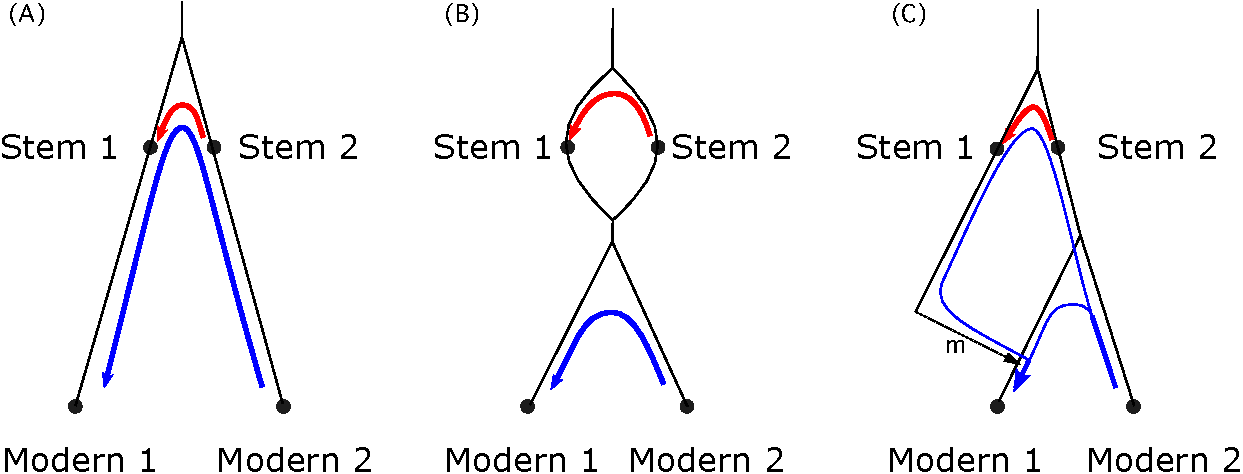
\includegraphics[width=0.75\textwidth]{figures/supp-f4-scenarios}
    \caption{
        \textbf{Present-day structure attributable to ancient population structure.}
        The statistic 
        $f_4(\text{stem}_1, \text{stem}_2; \text{present}_1, \text{present}_2)$
        captures how much of present-day population structure can be attributed to 
        population structure among the stems. The blue line represents genetic drift 
        along ancestral branches between contemporary populations, while the red line 
        represents drift between stem populations. $f_4$ measures the overlap 
        between the blue and red line, which corresponds to shared genetic drift 
        between the two pairs. 
        In scenario A, contemporary populations are descended from distinct stems, and 
        $f_4(\text{stem}_1, \text{stem}_2; \text{present}_1, \text{present}_2)$
        equals the drift between stems, $f_2(\text{stem}_1, \text{stem}_2)$.
        In scenario B, despite deep population structure, there is no shared drift
        and $f_4=0$. That is, present-day population structure is unrelated to
        structure among stems. In more realistic scenario C, where $\text{present}_1$
        receives a proportion $m$ of its ancestry from the dotted arrow, the overlap
        is only found along the corresponding path, and $f_4$ depends on both
        ancestry proportion $m$ and drift between stems,
        $f_4(\text{stem}_1, \text{stem}_2; \text{present}_1, \text{present}_2)
        = mf_2(\text{stem}_1, \text{stem}_2)$
    }
    \label{fig:supp-f4-scenarios}
\end{figure}

\subsection{Back-to-Africa Gene flow and Neanderthal ancestry in Africa} 

Back-to-Africa migrations likely introduced Neanderthal ancestry into Africa
\citep{Chen2020-wh}. This Neanderthal ancestry would cause reticulation in the
ancestry of the African populations, and is therefore relevant to the modeling
presented here. The models we inferred account for both Neanderthal admixture
in Eurasia and Back-to-Africa migrations, such that they predict the amount of
Neanderthal ancestry that we would expect to find in African individuals. We
find that African populations without high proportions of recent Eurasian
ancestry are predicted to carry $0.1-0.2\%$ Neanderthal
ancestry (Table~\ref{tab:supp-lineage-probabilitys}),
which is remarkably consistent with the results of
\citet{Chen2020-wh}. Since the IBD statistics from \citet{Chen2020-wh} are not
used in the present analysis, this serves as an independent validation of the
present models. More importantly, since the Neanderthal admixture in Africa is
properly accounted for in the model, we do not expect the presence of such
ancestry to bias our estimate of reticulation in Africa.

\subsection{Relating model predictions to morphological variation}
\label{sec:morpho_diff}

Here we show how the predictions of our model can be related to morphological
variation in the fossil record.
Let $\Delta^2$ be the expected squared difference in a morphological measurement
between fossil 1 and fossil 2,
\begin{equation}
    \Delta^2=\E\left[\left(\bar{X}_1-\bar{X}_2\right)^2\right]+\E\left[V_1\right]+\E\left[V_2\right],
\end{equation}
where $\bar{X}_1$ and $V_1$ and $\bar{X}_2$ and $V_2$ are measurement means and
variances for the populations from which fossil 1 and fossil 2 are sampled.

If we assume that the trait being measured is evolving neutrally, which seems
reasonable as an approximation based on studies of morphological (cranial)
variation in humans and Neanderthals
\citep{Relethford1994-mh,Weaver2008-ho,Von_Cramon-Taubadel2009-zb}, then
\begin{equation}
    \E\left[\left(\bar{X}_1-\bar{X}_2\right)^2\right]=4\sigma_m^2\tau_B-2\sigma_m^2\tau_{W_1}-2\sigma_m^2\tau_{W_2},
\end{equation}
\begin{equation}
    \E\left[V_1\right]=\frac{1}{h^2}\sigma_m^2\tau_{W_1},
\end{equation}
and
\begin{equation}
    \E\left[V_2\right]=\frac{1}{h^2}\sigma_m^2\tau_{W_2},
\end{equation}
where $\sigma^2_m$ is the additive genetic variance introduced by mutation
(per zygote per generation), $h^2$ is the (narrow sense) heritability,
$\tau_{W_1}$ and $\tau_{W_2}$ are the average coalescence time of pairs
of alleles from the same population, and $\tau_B$ is the average coalescence
time of pairs of alleles from different populations
\citep{Whitlock1999-un,Weaver2016-id}.
Substituting and simplifying gives
\begin{equation}
    \Delta^2=\sigma_m^2 \left( 4\tau_B+\frac{1-2h^2}{h^2} \left( \tau_{W_1}+\tau_{W_2} \right) \right),
\end{equation}
which relates $\Delta^2$ to between and within population coalescence times.

As a further approximation, if we assume that the heritability of the
measurement is close to one half, then
\begin{equation}
    \Delta^2\approx4\sigma_m^2\tau_B,
\end{equation}
which shows that under these assumptions $\Delta^2$ is proportional to $\tau_B$.

Nucleotide diversity, $\pi$, for pairs of individuals sampled from different
populations is also proportional to $\tau_B$.
Therefore, ratios of $\Delta^2$ can be predicted from ratios of $\pi$
for the same comparisons.
For example, a ratio for which $\pi$ for Stem 1 and Stem 2 is the numerator
and $\pi$ for a pair of contemporary human populations is the denominator
can be used to predict $\Delta^2$ for two fossils sampled from each of the
two stems based on $\Delta^2$ for contemporary humans.
In this way, the predictions of our model can be related to morphological
variation in the fossil record.

\section{Model validation strategy}
\label{sec:validation_strategy}
We took two approaches to validate demographic model inferences. First, we
explored the effects of using alternative populations, sample sets, and
recombination maps, and the effect of relaxing fixed parameters when fitting
the demographic models to diversity and LD statistics. We then use simulations
to test our inferred model predictions against other informative summary
statistics. Results are shown in the Supplementary Results
(Section~\ref{sec:supp-results}).

\subsection{Validations using alternative data sets and model specification}
\label{sec:validation-data-models}

\subsubsection{Alternate Thousand Genomes population sets}

In our primary model fits, we used the Mende in Sierra Leone (MSL) and the
British from England and Scotland (GBR). We tested the same models against a
different West African population (the Yoruba from Ibidan, Nigeria, YRI), and
two different European populations (Western Europeans from Utah, CEU, and
Toscani in Italy, TSI). The CEU are closely related to GBR and are thus likely
to be an equivalently close proxy for European ancestry in African individuals
with admixed European ancestry. The TSI are likely more distantly related to
the source of this European ancestry. We chose not to replace the GBR
by non-European Eurasian populations, as these would be poorer proxies for early
Holocene and recent colonial migration from the Near East and Europe back to
Africa, and it is unclear how such a model should be interpreted. We therefore
refit each of our best-fit demographic models using the following alternate
population sets: (Nama, YRI, Gumuz, Oromo/Amhara, and CEU), and (Nama, MSL,
Gumuz, Oromo/Amhara, and TSI).

\subsubsection{Variable thresholds of Nama-associated ancestry}

The Nama have recent European ancestry, and Nama individuals in our dataset
show varying levels of inferred ancestry relating to European populations
(Figure~\ref{fig:diversity}D, in the main text). Each of our inferred models
allows for gene flow from Eurasia to Africa after the out-of-Africa migration
event, through early Holocene back-to-Africa migration in East Africa, recent
colonial admixture in South Africa, and ongoing continuous migration between
branches leading to East African and European populations. While our
demographic models directly account for European ancestry in Nama individuals,
inferred parameters relating to early divergences and population structure may
be impacted by recent admixture.

To assess the impact of recent European admixture in Nama individuals on
inferred early divergence times and population structure, we subset the set of
Nama individuals that we included based on inferred European-matching ancestry
proportions. We used inferred ancestry proportions from \texttt{ADMIXTURE} with
the number of clusters $K=4$ (Section~\ref{sec:dimred}) and kept individuals
with either at least a) 90\% or b) 99\% proportion of inferred ancestry that
clusters within the Nama group (colored green in Figure~\ref{fig:diversity}D).
This left a) 18 Nama individuals with at least 90\% inferred South African
ancestry, and b) 14 Nama individuals with at least 99\%. For each subset, we
recomputed diversity and heterozygosity statistics and fit each of our
demographic models to these statistics.

\subsubsection{Varying fixed divergence times}
\label{sec:change_dates}
In order to reduce parameter space to avoid overfitting, we fixed parameters
that have previously been inferred, including the timings of the early
back-to-Africa migration contributing to the ancestry of East African
agricultural populations (12ka), the divergence of West and East Africans
(60ka), and the out-of-Africa migration event (50ka). Due to variability in
inference and dating methods, there is some uncertainty surrounding these
dates. We explored how variable timings of these events effect our inferred
models by 1) increasing the fixed times of the E-W African split (to 100ka) and
the out-of-Africa event (to 60ka), and 2) allowing those two parameters to be
jointly fit in model optimization.

\subsubsection{Recombination map inferred from Nama}

Throughout, we used inferred recombination maps based on the YRI OMNI array
data \citep{1000_Genomes_Project_Consortium2015-zq}. Because recombination
rates can vary between populations, we tested the robustness of our demographic
inference to the recombination map used to compute LD. We recomputed diversity
and LD statistics using recombination rates from the Nama recombination map
\citep{Van_Eeden2022-od}, and refit our best-fit demographic models to these
statistics.

\subsection{Validations using simulations from inferred demographic models}

Here we focus on four parameterizations of early human history: (1) a “single
origin” with recent expansion, (2) primary and second stem populations with
“continuous migration”, (3) two stem populations that do not exchange migrants
before merging to form regional African populations, referred to as a “merger
without stem migration”, and (4) two stem populations that are allowed to
exchange migrants before merging to form regional African populations, referred
to as a “merger with stem migration”. Given the best fit parameters for each
model
(Tables~\ref{tab:supp-single-origin}--\ref{tab:supp-merger-with-stem-migration}),
we used \msprime version 1.0.4 \citep{Kelleher2016-lw,Baumdicker2022-mj} to
simulate sampled individual genomes to match the data used in inference (see
simulation details below). We used these simulations to compare our model predictions to 
predictions based on the conditional SFS (cSFS) and on relate curves (see below).  

These comparisons serve as independent validations
of our inferred demographic models by assessing how well those models fit
aspects of the data that have been used in other studies as evidence of
population structure or archaic hominin admixture from an unidentified hominin species
within Africa.

\subsubsection{Simulation details}

The four inferred demographic models (single origin, continuous migration,
merger without stem migration, and merger with stem migration) were converted
to \demes format \citep{Gower2022-yn} and used as
the input demography for \msprime simulations. We sampled the same
number of individuals from each population as used in the inference (Nama: 44,
Mende: 85, Gumuz: 23, combined Oromo/Amhara: 46, British: 91, and Vindija
Neanderthal: 1). We assumed a generation time of 29 years, a per-base mutation
rate of $1.25\times10^{-8}$, a per-base recombination rate of $1\times10^{-8}$
(corresponding to 1cM/Mb), and we simulated 100 replicates with sequence
lengths of 50Mb per replicate. We computed the conditional site frequency
spectrum (cSFS) conditioned on observing the derived variant in the Neanderthal
sample, and reconstructed gene genealogies using \Relate to obtain coalescence
rate trajectories and distributions of deep branches passing through the
Neanderthal branch. Each analysis followed the same procedure as described
above in the analysis of the real data.

\subsubsection{cSFS prediction under inferred models}
\label{sec:misspecification}
We compared the observed cSFS to model predictions for the Nama, Mende, and
Gumuz populations. The cSFS from data is sensitive to ancestral allele
misidentification, but our simulations assume perfect knowledge of the
ancestral allele. To investigate the role of misidentification, we compared
predicted and observed cSFS for transitions and transversions separately as
well as jointly.

For each comparison, we fit a misidentification parameter $p_{misid}$ as well
as a scaled mutation rate $\theta$. The misidentification parameter is the
fraction $p_{misid}$ of loci that have the ancestral state misidentified.
Accounting for $p_{misid}$ mixes the predicted joint population SFS with a
small amount of the ancestral-allele-reversed SFS (i.e. for a two-population
joint SFS, $SFS_{misid}(i, j)=(1-p_{misid})*SFS(i, j) + p_{misid}*SFS(n-i,
m-j)$, where $n$ and $m$ are the sample sizes from the two populations). The
cSFS for the first population (conditioning on the second) is found by
projecting the sample size to $(n, 1)$ and taking $cSFS=SFS(:,1)$. $\theta$ and
$p_{misid}$ were chosen to maximize a likelihood assuming that each observed
entry in the cSFS is drawn from a Poisson distribution \citep{Sawyer1992-rt}.

\section{Model validation results}\label{sec:supp-results}
\label{sec:validation_results}
\subsection{Model fit using alternative datasets}
\label{sec:supp-alt-data}

All supplementary inference results discussed in this section are provided in
Demes format \citep{Gower2022-yn} as a supplemental zipped archive. For each
scenario, we refit the continuous migration and multiple merger models, with
stem migration.

\subsubsection{Replacing Thousand Genomes populations}
\label{sec:replacing}
We replaced the Mende (MSL) and British (GBR) population sets with Yoruba (YRI)
and Western and Northern Europeans (CEU), respectively, and refit our inferred
demographic models to diversity and LD statistics computed from those
populations (along with Nama, Oromo/Amhara, and Gumuz). Because the MSL and YRI
share recent West African ancestry, and the GBR and CEU share recent European
ancestry, we expected most parameters in inferred models using these two
datasets to be largely similar. Indeed, all parameters inferred using the YRI
and CEU data were well within one standard error of the same parameters
inferred using the MSL and GBR data, across all tested models. The one
exception to this was the recent size of the YRI branch, inferred to be
somewhat smaller than the final size of the analogous MSL branch ($\approx
20,000$ vs. $\approx 30,000$, resp.). Other population sizes, migration rates,
and divergence times were highly consistent.

Because CEU and GBR are genetically closely related, we also tested the
consistency of inferred parameters when replacing GBR with Toscani from Italy,
a more distantly related European population set than GBR. Most parameters in
each of the tested models were consistent with parameters inferred using GBR.
The only large difference was found in fitting the continuous migration model,
where the Nama divergence was $\approx200$ka rather than $135$ka. Our original
model using the dataset with GBR underestimated both $\sigma_{Dz}$ and
$\sigma_{\pi_2}$ compared to data
(Figure~\ref{fig:supp-continuous-migration-fits}), and as a result provided a
poorer fit to the data than the multiple merger model. When fitting this same
model to the TSI, the model provided a better fit to the $\sigma_{Dz}$
statistics but a worse fit to the $\sigma_{\pi_2}$ statistics (and still
provided a significantly worse fit to the data compared to the multiple
merger model). Migration rates during this early period of the model also
shifted to larger values between the stem populations, demonstrating that
divergence times and migration rates are confounded parameters in this model.
These differences in inferred parameters are likely driven by a combination of
factors: the continuous migration model mis-specifies historical dynamics in
the range of 100-200ka; the TSI are an inappropriate proxy for recent European
admixture in East and South Africa; and the TSI may also carry recent North
African ancestry, which is not captured in our model. By contrast, the
multiple merger model (which provides a better fit to the data) was inferred to
have consistent divergence and merger times between the models fit using GBR
and TSI, with ancestral populations ``reshuffling'' between 100 and 120ka.

In summary, across all validations to alternative datasets described in this
section, model fits were largely robust and matched those shown in the main
text (Figure~\ref{fig:best-fit-models})---the single outlier in these
validations was the estimated divergence time for the Nama in the continuous
migration model fit to the dataset that included TSI instead of GBR. Thus,
while specific aspects of the inferred demographic inference can be sensitive
to the choices of populations to include and the choices of model
specification, the results presented in the main text are broadly robust to
choices of model, dataset, and analysis choices. Our conclusions in the main
text took into account both this overall robustness and the important sources
of uncertainty. 

\subsubsection{Fit to LD statistics from Nama recombination map}

The LD statistics computed using the OMNI YRI recombination map and the
Nama-specific recombination map were very similar, with only a handful of
statistics showing slight visible differences
(Figure~\ref{fig:supp-omni-nama-comparison}). We therefore expected inferred
demographic models to be highly consistent when fit to the two sets of
statistics. Across each of our models, inferred parameters from fits using data
from the Nama-specific map were unchanged, with best-fit values all within one
estimated standard error from the inferred parameters from the OMNI YRI map.

Among human populations, the Nama are relatively highly diverged from the
sampled populations used in estimating the OMNI recombination maps (such as the
YRI), and the two recombination maps were inferred using different
computational methods from different types of sequencing data (arrays vs. whole
genomes). Therefore, differences between these two maps are likely near the
upper bound for differences in recombination rates between present-day human
populations \citep{Van_Eeden2022-od}. Because our fits were highly consistent
when using the two recombination maps, we conclude that inferences using the
diversity and LD statistics here are robust to variation in recombination rates
between present-day populations as well as to any differences in inferred
recombination rates due to true recombination rate differences or typical
statistical error in recombination rate estimation.

\subsubsection{Varying Nama ancestry-proportion thresholds}

In the demographic inference results presented in the main text, we did not
impose a minimum threshold on inferred Nama ancestry (as estimated using
ADMIXTURE). Because our proposed models allow for post-divergence gene flow as
well as recent admixture events, we can jointly learn deeper history and recent
admixture dynamics. This is in contrast to methods that do not account for
ongoing migration or recent admixture events, for which un-admixed genomes (if
they even exist) are needed for unbiased estimates of earlier history.
Although the methods used in this paper (\texttt{moments-LD}) are able to infer
early and recent history jointly, we tested the robustness of the inferred
early history to varying ancestry proportions in the Nama population. To do
this, we used ADMIXTURE to cluster inferred ancestry components, noting that
ADMIXTURE-inferred ancestries are coarse and can be misleading about true
underlying admixture proportions. Nonetheless, we included Nama individuals
that exceeded either $90\%$ or $99\%$ ancestry primarily shared among Nama
individuals.

For both thresholds, early history was robust in all tested models. Divergence
times and migration rates did not vary significantly from the original fits
that included all unrelated Nama individuals. The primary differences between
these fits and the original fits that did not impose an ancestry threshold were
the inferred admixture proportions of East African agriculturalists (2ka) and
Europeans (10 generations ago) in the Nama population. The East African
admixture proportion was reduced from $\approx 25\%$ to $20-22\%$, while the
European admixture proportion was reduced from $\approx 15\%$ to either $5-6\%$
(with a $90\%$ ancestry cutoff) or $3-5\%$ (with a $99\%$ ancestry cutoff). No
other parameters were strongly affected by subsetting the Nama individuals by
ADMIXTURE-inferred ancestry proportions. Because only the inferred proportions
of recent admixture in our model fits changed, we conclude that our inferences
of early history are robust to recent admixture, as long as that recent
admixture is accounted for in the demographic models.

\subsection{Relaxed inference of divergence times}
\label{sec:change-dates}

In the primary results presented in the main text
(Tables~\ref{tab:supp-single-origin}--\ref{tab:supp-merger-with-stem-migration}),
we fixed a number of parameters that have been previously inferred or are well
constrained by historical records (Section~\ref{sec:models}), including the
Eurasian out-of-Africa expansion at 50ka and the divergence of Western and
Eastern African groups at 60ka. To evaluate the effects of these choices on the
inference of other parameters in the model, we first fixed those modeled
divergence times to 60ka (for the out-of-Africa expansion) and 100ka (for the
E/W African divergence). In the next section, we allow those parameters to be
fit along with all other model parameters.

By fixing those divergence times to older dates, the inferred models preferred
older dates for the other free divergence time parameters. These dates were
stretched by a similar proportion that our fixed parameters were shifted, so
that the Nama divergence time was inferred to be $\approx150$ka, rather than
$\approx130$ka. Notably, older divergence times resulted in models with worse
likelihoods than our primary presented results. Overall, these inferred models
have a similar interpretation to the primary inference results, and the deep
population structure was unaffected by these choices.

When we allowed the out-of-Africa expansion and Eastern/Western African
divergence times to be jointly fit in model optimization, we found that the
best-fit inferred E/W divergence time and the OOA expansion were more recent
($45-55$ka and $35-40$ka, resp.). The remainder of the parameters were largely
unaffected by these shifts to more recent divergence times, and our
interpretation of the inferred early history remains unchanged. The $95\%$
confidence intervals around these parameters were relatively narrow ($\approx
5$ka for the OOA split, $\approx 10$ka for the East/West African split),
although this uncertainty does not capture uncertainty due to model
mis-specification (as discussed in Section~\ref{sec:models}).

\subsection{Alternative statistics for four models}

\subsubsection{Conditional SFS}
\label{sec:cSFS}
The single-origin model fit the cSFS relatively poorly across the three
populations compared to the models that allow structure between stem
populations (Fig.~\ref{fig:supp-csfs-single-origin}). The model that best fit
the cSFS was the merger-with-stem-migration model, which also provided the best
fit to pairwise diversity and LD statistics in the initial optimization. For
the Mende and Gumuz, the merger-with-stem-migration model fits the data very
well, while it underestimates rare variants in the Nama cSFS
(Fig.~\ref{fig:supp-csfs-merger-with-stem-migration}). Models learned from the
two-locus statistics provided a better qualitative description of the cSFS than
models previously fit directly to the cSFS  (see, e.g., figure 1 in
\citet{Durvasula2020-td}). We found that the inferred ancestral
misidentification rates were concordant across populations. The inferred rates
of ancestral misidentification were about twice as high for transitions
relative to transversions as expected, qualitatively, from the higher
transition mutation rate \citep{Hernandez2007-mf}.

\subsubsection{Relate curves from inferred models}
\label{inferred_relate}
We used \Relate \citep{Speidel2019-nj} to reconstruct gene genealogies from the
simulations under our four inferred demographic models. From each of these,
following the same approach as for the analysis of the actual data, we computed
coalescence rates within and between sampled populations. From the coalescence
rates, we estimated the inverse instantaneous coalescence rate (IICR, often
interpreted as an estimator of $N_e$) for each population, as well as relative
cross coalescence rates between pairs of populations.

The IICR is only a reliable estimator of $N_e$ in the absence of population structure.
However, since IIRC are readily estimated and visually interesting,
it is commonly attempted even when the assumption is not met.
Even if the assumption is not met, the inferred IIRC can be interpreted as a
summary statistic for which model predictions can be compared to data.
It can therefore be
informative about aspects of the data that our models fail to predict.
We also note that the coalescence rates inferred from data used a larger set of
populations from the combined 1000 Genomes/ADRP dataset, while our model
simulations only included a subset of 5 populations. This may lead to
differences in resolution of the inferences.

The data shows the characteristic ``hump'' of increased IICR ($N_e$) 100-300k
for all populations, followed by a decrease in size among all populations that
is sharpest in the Eurasian populations and also pronounced in the East African
populations that have high proportions of Eurasian ancestry (Amhara and Oromo)
(Fig.~\ref{fig:supp-iicr-data}). The model-inferred $N_e$ curves also show this
general trend for the more recent reduction in $N_e$
(Fig.~\ref{fig:supp-iicr-sim}). In the the more distant past, $N_e$ fluctuates
in a manner that is broadly similar across models with observed ``humps'' of
increased $N_e$. Despite the large differences in parameterizations and
interpretations of the four inferred demographic models, each of them show
reconstructed $N_e$ trajectories that are qualitatively similar, highlighting
the difficulty in learning complex demography in the deep past from
reconstructed coalescence rate trajectories.

We also compared the relative cross-coalescence rates (RCCR) between pairs of
populations in the four inferred demographic models
(Figures~\ref{fig:supp-rccr-single-origin}--\ref{fig:supp-rccr-merger-with-stem-migration})
to those in the data (Fig.~\ref{fig:supp-rccr-data}). In the recent past
($<$10ka), each of the models show increased RCCR compared to the data.
However, in the medium to more distant past, the RCCR provide a good match to
the data in each of the four models, including both their timing and ordering
of increased cross coalescences. The failure to match both the IIRC and RCCR in
the recent past in all models suggests that additional parameters would be
needed to account for recent increases in population sizes. As is the case with
other methods that reconstruct size history trajectories from inferred coalescence
rates (e.g. PSMC, MSMC), \Relate has difficulty inferring coalescences that
occur in the recent past.

\subsubsection{Distribution of deep branch affinities to Neanderthal sequence}

Following \citet{Speidel2019-nj}, we also characterized Neanderthal-matching
deep branches (see Section~\ref{sec:relate}) in our simulated data under the
four inferred demographic models. Comparing deep-branch distributions from the
data (Fig.~\ref{fig:supp-deep-branches}) to the models
(Fig.~\ref{fig:supp-deep-branches-sim}), we find consistent trends between each
of the four models and the data in the ordering of proportions of lineages from
each population that are labeled as Neanderthal-matching deep branches. This
proportion is slightly over-estimated in each of the African populations
compared to the data, but is closest in the merger-with-stem-migration model
(which also fit the LD statistics the best of the four highlighted models).
Given the qualitative discrepancies between the data IICR and the model IICR,
the differences in Neanderthal branch affinities is unsurprising.


\subsection{Re-inference of IM models from simulated data}
\label{sec:IM-reinfer}

Recent studies have focused on characterizing the timing of the earliest
divergences among human populations, and such analyses
typically fit simple isolation-with-migration (IM) or ``clean split'' models to
observed allele frequencies or inferred coalescence times among and between
populations (see \citet{Weaver2008-ho,Bergstrom2021-iw} for recent reviews).
Simple IM models
typically fit a constant $N_e$ within the two diverged population, the split
time, and a symmetric continuous migration rate (which could be fixed to zero,
equivalent to the ``clean split'' model). We explored the effect of fitting
such simplified models of history to data from more complex models by
simulating the site frequency spectrum (SFS) under each of our four models for
pairs of populations and reinferring an IM and clean split model for each pair.
The simulations sampled 10 diploid individuals from each
population, and we used \msprime \citep{Baumdicker2022-mj} to simulated
500 Mb of total sequence length (the sum over 500 replicates each 1 Mb in length)
with constant recombination rate $r=10^{-8}$ and mutation rate $u=2\times10^{-8}.$

As expected, the clean split models consistently provide divergence times $T$
that are more recent than the IM models. Because $T$ and subsequent migration
can be inversely confounded in SFS inference, fixing migration rates to zero
results in more recent inferred $T$ (Fig.~\ref{fig:supp-IM-misspecification}).
Even though each of our four models inferred divergences of all human
populations $\sim$120ka, ancient structure and size changes in the simulations
biases re-inferences and gives inflated estimates of $T$. Such an effect has
been shown to occur when the ancestral population size increases prior to the
population split \citep{Momigliano2021-th}, which is the case in our inferred
single-origin model. Re-inferred $T$ between the Nama and other populations
were $>$200ka under the IM model, and $\sim$50--130ka under the clean split
model.

To understand the relationship between model specification and demographic inference, 
consider the five toy models shown on Figure \ref{fig:toymodels}: A) clean split 100ka, 
B) clean split 200ka, C) population growth at 200ka followed by split 100ka, 
D) split 200ka followed by migration until 100ka, and E) split 200ka followed by 
merger 105ka and a new split 100ka. 

\begin{figure}[ht!]
    \centering
    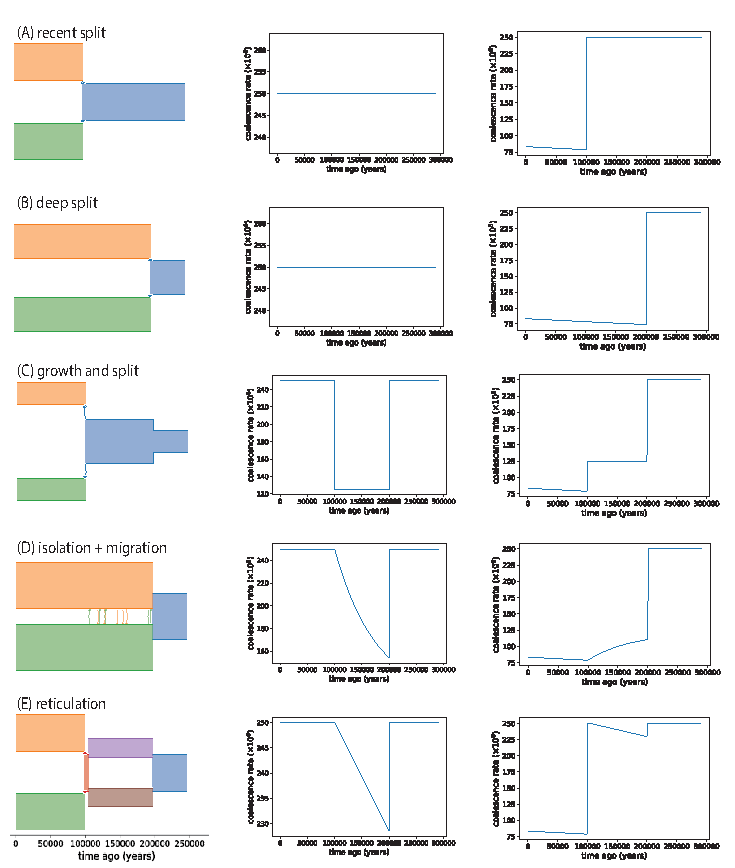
\includegraphics{figures/toy_models/toy_model_combo}
    \caption{
        \textbf{The impact of model specification on coalescence rate and
        inference.} We show five simplified demographic models that differ in
        demographic events, occurring between 200ka and 100ka, that mark the
        transition between a single ancestral population and two daughter
        populations. A: A clean split 100ka, B: A clean split 200ka, C:
        population growth at 200ka followed by split 100ka, D: split 200ka
        followed by migration until 100ka, and E: split 200ka followed by
        merger 105ka and a new split 100ka. The left column shows model
        representation, the middle column shows instantaneous coalescence rates
        for pairs of lineages from the same daughter population, the right
        column shows instantaneous coalescence rates for pairs of lineages
        coming from distinct populations.  
    }
    \label{fig:toymodels}
\end{figure}

Models C), D), and E) show qualitatively similar patterns of coalescence rate. 
Given the same data, an IM model (such as D) will infer a potentially much 
deeper population divergence than growth model C and reticulation model E.

\subsection{Batch effects from merged data biases inference}
\label{sec:merged-bias}

Merging samples from multiple independently called datasets can cause
systematic biases in computed diversity statistics (i.e., batch effects). In
order to explore the severity of batch effects on the LD statistics used in our
inferences, we took advantage of multiple independently sequenced and called
datasets using the same individuals from the Thousand Genomes project. We used
the phase 3 low coverage \citet{1000_Genomes_Project_Consortium2015-zq} data
and the high coverage resequenced data of the same individuals
\citep{Byrska-Bishop2021-jl} to 1) verify that computed diversity statistics
and inferences are robust to low coverage data, and 2) demonstrate that merging
data without joint variant calling can lead to substantial biases in inferred
demographic parameters. We analyzed two populations, the Mende (MSL) and
British (GBR), and considered a two-population isolation-with-migration model.

We computed four sets of diversity and LD statistics, one set of statistics
from the jointly called high coverage data, one from the jointly called low
coverage data, and one each from merged high and low coverage (MSL high
coverage and GBR low coverage; and GBR high coverage and MSL low coverage).
Using the measurement variances from each two-locus statistic in the high
coverage data, we estimated measurement error of the other three sets of
statistics (low/low, low/high, and high/low) against the high coverage data.
The jointly called low coverage data provided statistics that closely matched
the high coverage statistics, with each statistic within 1--2 standard errors.
On the other hand, both the merged datasets provided statistics that deviated
from the jointly called data, particularly for the cross-population statistics
(Figure~\ref{fig:supp-merged-data-SEs}.

\begin{figure}[ht!]
    \centering
    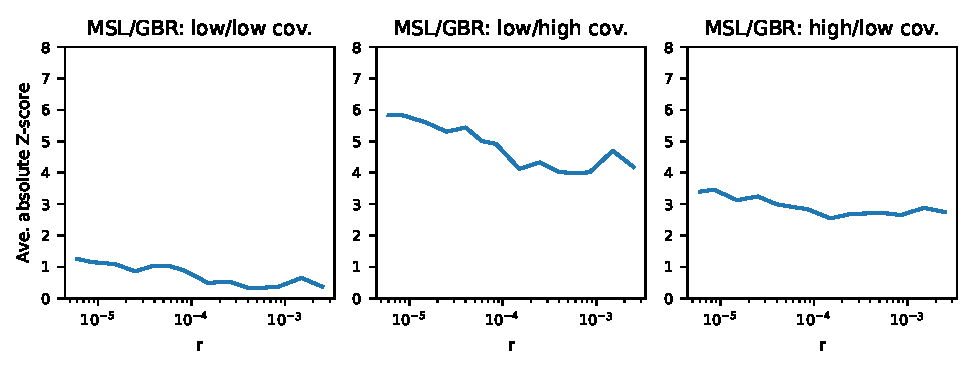
\includegraphics[width=5in]{figures/supp-SE-merged-data}
    \caption{
        \textbf{Average error of statistics from low coverage and merged
        datasets.} Low coverage data provides allelic diversity and linkage
        disequilibrium measures consistent with those from high coverage data
        (left panel). On the other hand, merging separately called datasets can
        lead to large discrepancies in computed LD statistics (middle and right
        panels).
    }
    \label{fig:supp-merged-data-SEs}
\end{figure}

With the observation that the low and high coverage data provided broadly
consistent statistics while the merged data provided inconsistent statistics,
we next wanted to assess whether their differences affect model inference. To
do this, we fit a two-population demographic model to the diversity and LD
statistics as described in Section~\ref{sec:optimization}. The modest
differences between the low and high coverage did not result in noticeable
differences in the optimized model (with an MSL-GBR inferred divergence time of
60ka, consistent with previous genomics studies). On the other hand, both
merged datasets provided substantially inconsistent fits, both to the high and
low coverage data and to each other. Notably, the inferred divergence time is
significantly older, due to the overestimation of mutational differences
between populations due to batch effects.

\begin{figure}[htb!]
    \centering
    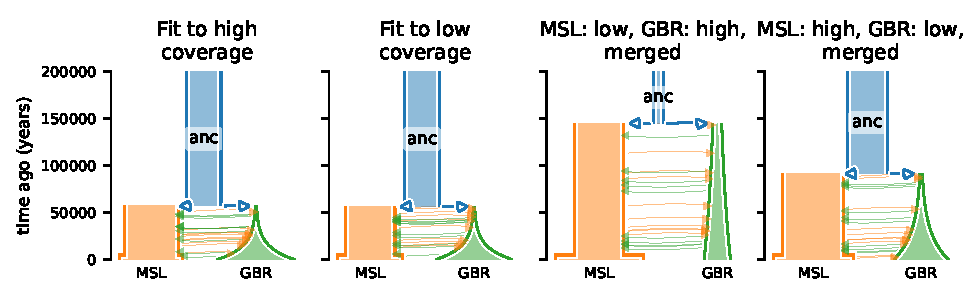
\includegraphics{figures/supp-merged-data-model-fits}
    \caption{
        \textbf{Merged datasets bias demographic inferences.}
        The panels represent best-fit models according to 
        different combinations of high- and low- coverage data.
        While statistics from low and high coverage datasets provide consistent
        best-fit demographic models, merged datasets result in biased LD
        statistics (Figure~\ref{fig:supp-merged-data-SEs}). These biased LD
        statistics lead to large downstream biases in inferred demographic
        models. 
    }
    \label{fig:supp-merged-data-fits}
\end{figure}

More careful post-merging quality control may alleviate some of these
discrepancies. However, low coverage data provides a consistent model fit to
the high coverage data. Therefore, it is preferable to favor jointly called low
coverage data over a mix of high coverage but separately called data, at least
when using the diversity and LD statistics that we have in our analyses.

\subsection{Model choice from likelihood differences}
\label{sec:refit-simulated-data}

The set of models we tested with the full dataset have varying complexity,
ranging from a single origin expansion to multiple stem populations connected
by migration and gene flow. Thus, our models have varying numbers of parameters
($21$ in the simplest model, and $30$ in the most heavily parameterized). Our
analyses found that the more complex models (multiple stems with ongoing
migration) provided the best fit to the data. To ensure that these more complex
models are not simply fitting noise in our data, we simulated data under both
simpler and more complex models, with same sample sizes and similar genome
length to that used in this study. From these, we fit each of our models and
checked that the correct model was chosen.

While simulations of datasets of this size are rapid, computing LD statistics
is computationally burdensome. We simulated 500 1Mb regions under our best fit
single origin, continuous migration, and merger with stem migration models.
Using these simulated regions, we constructed 500 bootstrap replicate datasets
by sampling with replacement. Each of these 500 replicate sets were fit using
the models reported in the main text, and we compared log-likelihoods across
each fit (Figure~\ref{fig:refit-lls}). The correct model was recovered in the
vast majority of cases based on log-likelihoods alone
(Table~\ref{tab:confusion-matrix}). We conclude that our inferences are not
simply fitting statistical noise, and the observed differences in
log-likelihoods indicate a better recapitulation of the true history.

\begin{table}[ht]
    \caption{
        \label{tab:confusion-matrix}
        \textbf{Model choice from fits to simulated data.} We simulated three
        models, based on the best fit parameters from fits to data. Using these
        simulated datasets, we reinferred four models that we tested in our
        analyses in the main text, including simple (single origin) and complex
        models. Among 500 fits, we almost exclusively recover the simulated
        model, even when fitting more complex (i.e., more heavily
        parameterized) models to simpler simulated models (such as the single
        origin model).
    }
    \centering
    \begin{tabular}[t]{lcccc}
        \toprule
        Simulated model & Single origin & Cont. migration & Merger w/out stem mig. & Merger w/stem mig. \\
        \midrule
        Single origin & 500 & 0 & 0 & 0 \\
        Cont. migration & 0 & 500 & 0 & 0 \\
        Merger w/stem mig. & 0 & 0 & 10 & 490 \\
        \bottomrule
    \end{tabular}
\end{table}

The single origin model is nested within the more complex models (with
migration from the additional stem population fixed to zero), those more
complex models can always recover the log-likelihood found by the single origin
model. We therefore explored the broader parameter space that included gene
flow from the additional stem population. In these fits, the optimization
converged either back to the nested single origin model (in which case the
single origin model was chosen), or it found a local optimum with lower
log-likelihood than the simpler model (see first panel in
Figure~\ref{fig:refit-lls}).

\begin{figure}[htb]
    \centering
    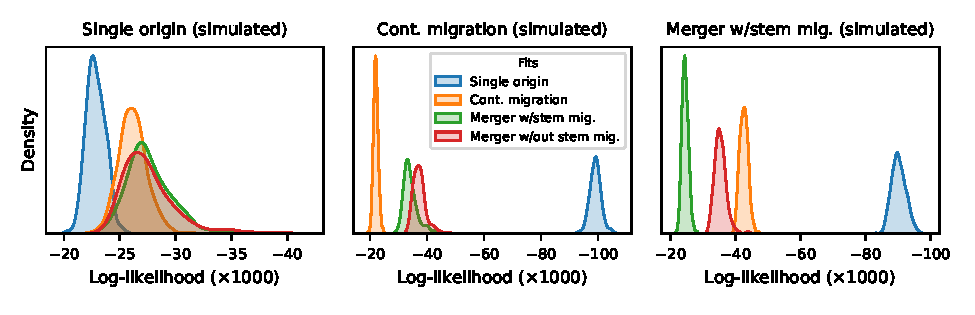
\includegraphics{./figures/supp-refit-lls.pdf}
    \caption{
        \textbf{Log-likelihoods of fits of four models to simulated data.} In
        three scenarios, a simple single origin model and our preferred
        continuous migration and merger with stem migration models, we
        simulated 500 replicates of 500 Mb with the same populations and sample
        sizes from our reported best fit models. We then fit the four models
        reported in the main text to each of these simulated datasets and
        compared log-likelihoods. In each case, the simulated model is
        correctly chosen, even under the single origin scenario. We conclude
        our more complex models (with more parameters) are not simply fitting
        statistical noise.
    }
    \label{fig:refit-lls}
\end{figure}

\subsection{Evaluation of confidence intervals}
\label{sec:bootstrap-CIs}

We created 200 block-bootstrap replicate datasets and refit our four reported
models to each replicate (Section~\ref{sec:likelihoods-uncertainty}). From
these refit models, we estimated the empirical uncertainty by taking the
standard deviation of the distribution of each refit parameter. We compared
these to our estimated standard errors from the Godambe Information Matrix
(GIM) approach to check that the confidence intervals from the GIM approach do
not underestimate true uncertainty (Table~\ref{tab:supp-confidence-intervals}).

The GIM-computed standard errors are generally close to those from the fits to
the bootstrap data, and some are larger (roughly 2--5x) than those from the
bootstrap fits. A possible explanation for this discrepancy is that some
parameters of our models come close to the lower and upper bounds allowed for
those parameters (e.g., small recent population size in the Nama, a bottleneck
in one of the stems). In such cases, the distribution of
parameters under constraints, and that of other correlated parameters in the model
may be narrower than
the true (unconstrained) uncertainties in those parameters. 
%Model constraints and parameter
%bounds in optimization may also lead to parameters fits that are away from
%their true optimal value. In this case, the GIM-estimated confidence intervals
%should be larger and contain what would be found from an unconstrained fit.

To demonstrate this effect, we simulated data under a simple
isolation-with-migration model, in which population sizes are allowed to vary,
and one population has a severe bottleneck in the most recent 1000 years
(Figure~\ref{fig:supp-uncerts-toy}). We simulated 200 1Mb regions with
$u=r=10^{-8}$, sampling 10 diploid individuals from each present-day population
and computed LD statistics. From these, we inferred the best fit parameters
without imposing bounds on the parameters, and we also reinferred the model
imposing a lower bound of 300 on population sizes (the bottleneck size). From
our fits, we computed confidence intervals using the Fisher information matrix
(FIM) and GIM approaches, in both the unbounded and bounded fits. We also
reinferred parameters over 200 bootstrapped replicate datasets to compare
empirical uncertainties to those estimated CIs.

As expected the FIM CIs underestimate the true uncertainty and the GIM CIs
closely match empirical uncertainty from the bootstrap fits. In the fit that
imposed a lower bound on population sizes, some GIM-estimated standard errors
were larger than those from the unbounded fits.  However, the fit parameters
were slightly shifted from the unbounded fits, due to hitting the lower bound
of the bottleneck size. In these cases, the estimated CIs were larger but
contained the true CIs from the unbounded GIM and bootstrap fits. For parameters
that were not strongly affected by hitting the bounds, the CIs matched closely
(Figure~\ref{fig:supp-uncerts-toy}).

\begin{figure}[htb]
    \centering
    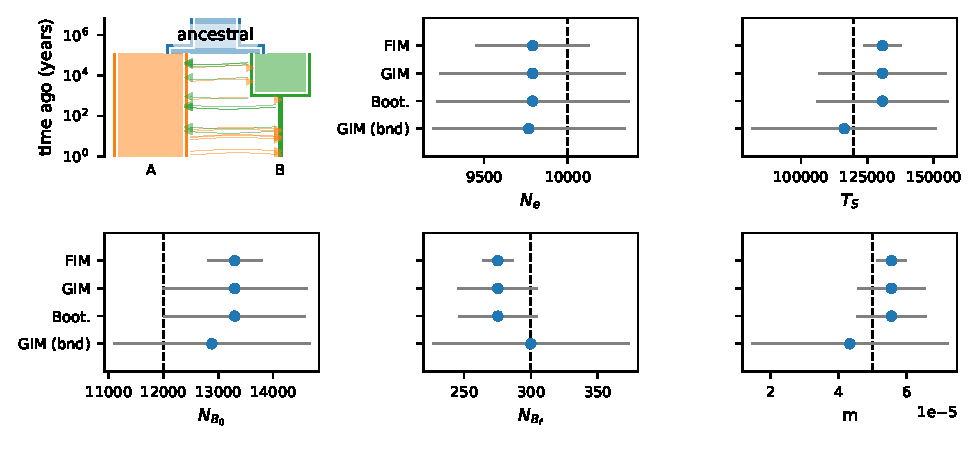
\includegraphics{./figures/supp-uncerts-toy.pdf}
    \caption{
        \textbf{Evaluation of GIM confidence intervals using moments-LD.}
        The GIM approach accurately estimates confidence intervals, accounting
        for non-independence between regions of linked loci. GIM-estimated CIs
        from the constrained fit are large enough to contain the true
        uncertainty. Vertical dashed lines indicate simulated parameter values.
    }
    \label{fig:supp-uncerts-toy}
\end{figure}

\subsection{Allowing for additional migrations}

In preliminary analyses, we found that inferred migration rates between the
Nama and non-East African groups were orders of magnitude smaller than
migration rates between other populations included in our inferences.
Therefore, to reduce the number of parameters needing to be fit we fixed those
rates to zero in subsequent fits, and our reported best-fit models did not
include migration between the Mende and Eurasians, nor between the Nama and
Eurasian populations (aside from recent colonial-period admixture). To assess
the impact of this choice, we re-inferred four of our reported models (single
origin, continuous migration, and merger with and without stem migration),
while allowing for additional parameters to include continuous, symmetric
migration for the duration of the coexistence of the Nama and Mende of the Nama
and British.

Indeed, the inferred migration rates for both of these pairs of populations
were small, with $2N_em \ll 1$ in all cases. In the single origin model, the
Mende-British migration rate was 1.04E-6 ($2N_em = 0.02$) and the Nama-British
rate was 2.67E-6 ($2N_em = 0.05$). In the continuous migration model, these
rates were 2.69E-6 ($2N_em = 0.038$) and 3.38E-6 ($2N_em = 0.048$), resp. In
the merger without stem migration model, these rates were 2.96E-6 ($2N_em =
0.064$) and 5.46E-6 ($2N_em=0.119$), resp. And in the merger with stem
migration model, these rates were 2.64E-6 ($2N_em = 0.055$) and 3.19E-6 ($2N_em
= 0.066$), resp. In comparison with other migration rates, with $2N_em \gtrsim
1$, these migrations have negligible impact on underlying statistics. The fits
to other parameters were negligibly different from those reported with these
migrations fixed to zero, and log-likelihoods were unimproved.

\subsection{Replacing the reference population for statistics normalization}

We used observed $\pi_2$ and pairwise diversity in the Mende to normalize two-
and one-locus statistics (see Section~\ref{sec:supp-ld-stats}). To confirm that
this choice of normalization did not impact inferred model parameters, we reran
each of our reported models using data normalized by $\pi_2$ and pairwise
diversity in the Gumuz. As expected, the best fit parameters from fits using
the Gumuz-normalized data were very close to those reported in
Tables~\ref{tab:supp-single-origin}--\ref{tab:supp-merger-with-stem-migration},
and they were all well within the reported confidence intervals. Our results
are therefore unlikely to be sensitive to this choice of normalization.

Reinferred demographic models from this and preceding sections are reported in
Demes format \citep{Gower2022-yn} as a supplemental archive.

\section{Mutation versus recombination rates}
\label{sec:supp-mutation}

Prior studies primarily relied on the mutation clock in order to date events
such as population divergence, and uncertainty about the mutation rate
translates in uncertainty in timing estimates (e.g., \citet{Moorjani2016-qj}).
Recent whole genome sequencing studies from non-pathological pedigrees have
typically estimated mutation rates to be $1.2-1.3\times10^{-8}$ per site per
generation \citep{Sasani2019-zp,Tian2019-zv}. A rate of $1.3\times10^{-8}$ also
approximates the rate predicted by a mutational model from gnomAD
\citep{Karczewski2020-le} in the $\sim$650Mb of intergenic regions selected for
demographic inference in this study.
\texttt{moments-LD} differs from other approaches by
relying on a recombination clock, which has been argued to be more robust to
estimation than a mutational clock \citep{Moorjani2016-ur}.

From our recombination-rate-calibrated demographic models, we can estimate the
mutation rates needed to fit patterns of pairwise diversity. With our best-fit
model (merger-with-stem-migration,
Table~\ref{tab:supp-merger-with-stem-migration}), a mutation rate of
$1.33\times10^{-8}$ recovers the observed diversity within and between
populations, closely matching the average mutation rate estimated from the
gnomAD mutation model. The other inferred demographic models
(Tables~\ref{tab:supp-single-origin}--\ref{tab:supp-merger-without-stem-migration})
would require mutation rates of $1.75-1.90\times10^{-8}$ to match pairwise
diversity.



\addcontentsline{toc}{section}{References}
\bibliographystyle{genetics}
\bibliography{paper}

\clearpage

\addcontentsline{toc}{section}{Supporting tables and figures}
\section*{Supporting tables and figures}

\begin{table}[ht]
    \caption{
        \label{tab:fixed-params}
        \textbf{Fixed parameters in inferred demographic models.}
        Many of the fixed parameters are specific to the Neanderthal branch, are
        constrained by known history, or were consistently fit across multiple
        model parameterizations. We assumed a generation time of 29 years throughout.
        See Section~\ref{sec:models} for details.
    }
    \centering
    \begin{tabular}[t]{rP{8cm}c}
        \toprule
        Parameter & Description & Value \\
        \midrule
        $T_{MH-Neand}$ & The time of the split between branches leading to Neanderthals and humans & 550ka \\
        $T_{NI-Vin}$ & The time of the split between branches leading to the Vindija sample and the Neanderthal population that mixed with expanding humans & 80ka \\
        $T_{Vin}$ & The sample time of the Vindija Neanderthal individual & 50ka \\
        $T_{NI\rightarrow EUR}$ & The timing of admixture from Neanderthals to humans & 45ka \\
        $f_{NI\rightarrow EUR}$ & The proportion of admixture from Neanderthals to humans & 0.015 \\
        $T_{E-W}$ & The split time of East and West African populations & 60ka \\
        $T_{GBR}$ & The split time of Eurasian and East African populations & 50ka \\
        $T_{GBR\rightarrow EA}$ & The time of the back-to-Africa admixture event, giving rise to the Amhara/Oromo branch & 12ka \\
        $T_{expan}$ & The expansion time of the Mende and contraction time of the Gumuz & 5ka \\
        $T_{EA\rightarrow Nama}$ & The admixture time of East African pastoralists to the Nama & 67 gen. \\
        $T_{GBR\rightarrow Nama}$ & The admixture time of Europeans to the Nama & 10 gen. \\
        $T_{bottle}$ & The bottleneck time of the Nama population & 9 gen. \\
        \bottomrule
    \end{tabular}
\end{table}


\begin{table}[ht]
\caption{
    \label{tab:supp-single-origin}
    \textbf{Best-fit parameters from the single-origin model.}
    This model includes a single stem population that splits into contemporary human
    groups. Fixed parameters are specified in Table~\ref{tab:fixed-params}.
    Inferred values are scaled to physical units assuming a generation time of
    29 years. This model gave a log-likelihood of -189,434.
}
\centering
\begin{tabular}[t]{rP{8cm}cc}
    \toprule
    Parameter & Description & Value & Std. err.\\
    \midrule
    $N_e$ & Ancestral effective population size & 10198 & 403 \\
    $N_{MH}$ & Size of human lineage between Neanderthal and Nama splits & 21111 & 529 \\
    $N_{Nama_0}$ & Initial Nama size & 10224 & 370 \\
    $N_{Nama_F}$ & Final Nama size & 222 & 9 \\
    $N_{MSL_0}$ & Initial Mende size & 17211 & 769 \\
    $N_{MSL_F}$ & Final Mende size & 16822 & 606 \\
    $N_{EA}$ & Size of East African branch & 7139 & 273 \\
    $N_{Gumuz_F}$ & Final Gumuz size & 3831 & 131 \\
    $N_{EP}$ & East African agriculturist size & 13033 & 491 \\
    $N_{GBR_0}$ & Initial British size & 846 & 33 \\
    $N_{GBR_F}$ & Final British size & 12121 & 507 \\
    $N_{Neand}$ & Neanderthal size & 1867 & 105 \\
    $T_{Nama}$ & Nama split time (years) & 110400 & 2525 \\
    $m_{Nama-MSL}$ & Nama--Mende symmetric migration rate & $2.82\times10^{-5}$ & $0.158\times10^{-5}$ \\
    $m_{Nama-EA}$ & Nama--East Africa symmetric migration rate & $4.94\times10^{-5}$ & $0.197\times10^{-5}$ \\
    $m_{MSL-EA}$ & Mende--East Africa migration rate & $18.76\times10^{-5}$ & $0.764\times10^{-5}$ \\
    $m_{EA-GBR}$ & East Africa--Europe migration rate & $4.42\times10^{-5}$ & $0.239\times10^{-5}$ \\
    $m_{EA-EA}$ & Intra-East Africa migration rate & $41.28\times10^{-5}$ & $1.33\times10^{-5}$ \\
    $f_{GBR \rightarrow EP}$ & Ancestry proportion of East African agriculturalists from GBR 12ka ($1-f$ from Gumuz) & 0.658 & 0.0039 \\
    $f_{EP \rightarrow Nama}$ & Ancestry proportion from EA pastoralists to Nama 2ka & 0.279 & 0.0039 \\
    $f_{GBR \rightarrow Nama}$ & Ancestry proportion from Europeans to Nama 10 generations ago & 0.150 & 0.0019 \\
    \bottomrule
\end{tabular}
\end{table}

\begin{table}[ht]
\caption{
    \label{tab:supp-continuous-migration-no-mig}
    \textbf{Best-fit parameters from the Continuous-Migration model without stem migration.}
    Inferred values are scaled to physical units assuming a generation time of
    29 years. This model gave a log-likelihood of -126,644. This model allows for
    continuous migration between Stem 2 and contemporary populations, but disallows
    migration between Stem 2 and Stem 1, which later splits into branches leading
    to South, East, and West African populations.
}
\centering
\begin{tabular}[t]{rP{8cm}cc}
    \toprule
    Parameter & Description & Value & Std. err.\\
    \midrule
    $N_e$ & Ancestral effective population size & 10543 & 460 \\
    $N_{stem1}$ & Size of stem 1 lineage between Neanderthal and Nama splits & 15297 & 1227 \\
    $N_{stem2}$ & Size of stem 2 lineage & 9156 & 573 \\
    $N_{Nama_0}$ & Initial Nama size & 11329 & 423 \\
    $N_{Nama_F}$ & Final Nama size & 219 & 11 \\
    $N_{MSL_0}$ & Initial Mende size & 11187 & 644 \\
    $N_{MSL_F}$ & Final Mende size & 24056 & 945 \\
    $N_{EA}$ & Size of East African branch & 7185 & 293 \\
    $N_{Gumuz_F}$ & Final Gumuz size & 3746 & 184 \\
    $N_{EP}$ & East African agriculturist size & 13187 & 645 \\
    $N_{GBR_0}$ & Initial British size & 937 & 41 \\
    $N_{GBR_F}$ & Final British size & 11478 & 420 \\
    $N_{Neand}$ & Neanderthal size & 2285 & 113 \\
    $T_{stems}$ & Stem split time (years) & 459720 & 21704 \\
    $T_{Nama}$ & Nama split time (years) & 139725 & 3250 \\
    $m_{Nama-MSL}$ & Nama--Mende symmetric migration rate & $1.93\times10^{-5}$ & $0.360\times10^{-5}$ \\
    $m_{Nama-EA}$ & Nama--East Africa symmetric migration rate & $4.43\times10^{-5}$ & $0.309\times10^{-5}$ \\
    $m_{MSL-EA}$ & Mende--East Africa migration rate & $20.8\times10^{-5}$ & $0.97\times10^{-5}$ \\
    $m_{EA-GBR}$ & East Africa--Europe migration rate & $4.46\times10^{-5}$ & $0.171\times10^{-5}$ \\
    $m_{EA-EA}$ & Intra-East Africa migration rate & $35.4\times10^{-5}$ & $1.85\times10^{-5}$ \\
    $f_{GBR \rightarrow EP}$ & Ancestry proportion of East African agriculturalists from GBR 12ka ($1-f$ from Gumuz) & 0.649 & 0.0038 \\
    $f_{EP \rightarrow Nama}$ & Ancestry proportion from EA pastoralists to Nama 2ka & 0.268 & 0.0048 \\
    $f_{GBR \rightarrow Nama}$ & Ancestry proportion from Europeans to Nama 10 generations ago & 0.153 & 0.0022 \\
    $m_{stems}$ & Stem 1--stem 2 migration rate & $0$ & fixed \\
    $m_{stem2-Nama}$ & Stem 2--Nama migration rate & $4.33\times10^{-5}$ & $0.891\times10^{-5}$ \\
    $m_{stem2-MSL}$ & Stem 2--Mende migration rate & $11.3\times10^{-5}$ & $1.83\times10^{-5}$ \\
    $m_{stem2-EA}$ & Stem 2--East Africa migration rate & $2.77\times10^{-5}$ & $0.699\times10^{-5}$ \\
    \bottomrule
\end{tabular}
\end{table}

\begin{table}[ht]
\caption{
    \label{tab:supp-continuous-migration}
    \textbf{Best-fit parameters from the Continuous-Migration model.}
    Inferred values are scaled to physical units assuming a generation time of
    29 years. This model gave a log-likelihood of -115,500.
}
\centering
\begin{tabular}[t]{rP{8cm}cc}
    \toprule
    Parameter & Description & Value & Std. err.\\
    \midrule
    $N_e$ & Ancestral effective population size & 7270 & 1777 \\
    $N_{stem1}$ & Size of stem 1 lineage between Neanderthal and Nama splits & 8256 & 1612 \\
    $N_{stem2}$ & Size of stem 2 lineage & 13547 & 2488 \\
    $N_{Nama_0}$ & Initial Nama size & 11939 & 2989 \\
    $N_{Nama_F}$ & Final Nama size & 221 & 54 \\
    $N_{MSL_0}$ & Initial Mende size & 9738 & 2479 \\
    $N_{MSL_F}$ & Final Mende size & 28150 & 6628 \\
    $N_{EA}$ & Size of East African branch & 7489 & 1841 \\
    $N_{Gumuz_F}$ & Final Gumuz size & 3728 & 915 \\
    $N_{EP}$ & East African agriculturist size & 13072 & 3246 \\
    $N_{GBR_0}$ & Initial British size & 959 & 231 \\
    $N_{GBR_F}$ & Final British size & 11822 & 2889 \\
    $N_{Neand}$ & Neanderthal size & 2670 & 591 \\
    $T_{stems}$ & Stem split time (years) & 1163072 & 390803 \\
    $T_{Nama}$ & Nama split time (years) & 134745 & 17775 \\
    $m_{Nama-MSL}$ & Nama--Mende symmetric migration rate & $0.98\times10^{-5}$ & $0.366\times10^{-5}$ \\
    $m_{Nama-EA}$ & Nama--East Africa symmetric migration rate & $4.08\times10^{-5}$ & $1.02\times10^{-5}$ \\
    $m_{MSL-EA}$ & Mende--East Africa migration rate & $21.4\times10^{-5}$ & $5.32\times10^{-5}$ \\
    $m_{EA-GBR}$ & East Africa--Europe migration rate & $4.17\times10^{-5}$ & $1.02\times10^{-5}$ \\
    $m_{EA-EA}$ & Intra-East Africa migration rate & $33.6\times10^{-5}$ & $8.35\times10^{-5}$ \\
    $f_{GBR \rightarrow EP}$ & Ancestry proportion of East African agriculturalists from GBR 12ka ($1-f$ from Gumuz) & 0.642 & 0.0037 \\
    $f_{EP \rightarrow Nama}$ & Ancestry proportion from EA pastoralists to Nama 2ka & 0.255 & 0.0043 \\
    $f_{GBR \rightarrow Nama}$ & Ancestry proportion from Europeans to Nama 10 generations ago & 0.156 & 0.0021 \\
    $m_{stems}$ & Stem 1--stem 2 migration rate & $6.43\times10^{-5}$ & $1.05\times10^{-5}$ \\
    $m_{stem2-Nama}$ & Stem 2--Nama migration rate & $5.82\times10^{-5}$ & $1.60\times10^{-5}$ \\
    $m_{stem2-MSL}$ & Stem 2--Mende migration rate & $16.4\times10^{-5}$ & $4.19\times10^{-5}$ \\
    $m_{stem2-EA}$ & Stem 2--East Africa migration rate & $3.10\times10^{-5}$ & $0.901\times10^{-5}$ \\
    \bottomrule
\end{tabular}
\end{table}

\begin{table}[ht]
\caption{
    \label{tab:supp-merger-without-stem-migration}
    \textbf{Best-fit parameters from the Merger-Without-Stem-Migration model.}
    Inferred values are scaled to physical units assuming a generation time of
    29 years. This model gave a log-likelihood of -107,652.
}
\centering
\begin{tabular}[t]{rP{8cm}cc}
    \toprule
    Parameter & Description & Value & Std. err.\\
    \midrule
    $N_e$ & Ancestral effective population size & 11258 & 326 \\
    $N_{stem1}$ & Size of stem 1 lineage between stem 1--stem 2 split and stem 1E--stem 1S split & 113 & 76 \\
    $N_{stem2}$ & Size of stem 2 lineage & 23984 & 1149 \\
    $N_{Nama_0}$ & Initial Nama and stem 1S size & 13134 & 384 \\
    $N_{Nama_F}$ & Final Nama size & 225 & 7.3 \\
    $N_{MSL_0}$ & Initial Mende size & 11856 & 322 \\
    $N_{MSL_F}$ & Final Mende size & 25558 & 987 \\
    $N_{EA}$ & Size of East African and stem 1E branch & 9136 & 246 \\
    $N_{Gumuz_F}$ & Final Gumuz size & 3385 & 102 \\
    $N_{EP}$ & East African agriculturist size & 13650 & 408 \\
    $N_{GBR_0}$ & Initial British size & 931 & 29 \\
    $N_{GBR_F}$ & Final British size & 12064 & 334 \\
    $N_{Neand}$ & Neanderthal size & 1935 & 91 \\
    $T_{stems}$ & Stem split time (years) & 420881 & 27380 \\
    $T_{stem1}$ & Stem 1 split time into stem 1E and stem 1S (years) & 367434 & 19952 \\
    $m_{Nama-MSL}$ & Nama--Mende symmetric migration rate & $0.361\times10^{-5}$ & $0.113\times10^{-5}$ \\
    $m_{Nama-EA}$ & Nama--East Africa symmetric migration rate & $4.00\times10^{-5}$ & $0.130\times10^{-5}$ \\
    $m_{MSL-EA}$ & Mende--East Africa migration rate & $19.5\times10^{-5}$ & $0.548\times10^{-5}$ \\
    $m_{EA-GBR}$ & East Africa--Europe migration rate & $3.77\times10^{-5}$ & $0.152\times10^{-5}$ \\
    $m_{EA-EA}$ & Intra-East Africa migration rate & $37.1\times10^{-5}$ & $1.26\times10^{-5}$ \\
    $f_{GBR \rightarrow EP}$ & Ancestry proportion of East African agriculturalists from GBR 12ka ($1-f$ from Gumuz) & 0.647 & 0.0037 \\
    $f_{EP \rightarrow Nama}$ & Ancestry proportion from EA pastoralists to Nama 2ka & 0.257 & 0.0042 \\
    $f_{GBR \rightarrow Nama}$ & Ancestry proportion from Europeans to Nama 10 generations ago & 0.156 & 0.0021 \\
    $m_{stems}$ & Stem 1--stem 2 migration rate & $0$ & fixed \\
    $T_{Nama}$ & Time of Nama merger event & 117392 & 8253 \\
    $f_{stem 2 \rightarrow Nama}$ & Proportion of stem 2 ancestry making up initial Nama lineage ($1-f$ from stem 1S) & 0.707 & 0.0086 \\
    $T_{EA}$ & Time of East Africa merger event & 94892 & 3648 \\
    $f_{stem 2 \rightarrow EA}$ & Proportion of stem 2 ancestry making up initial East Africa lineage ($1-f$ from stem 1E) & 0.481 & 0.0074 \\
    $T_{MSL}$ & Time of secondary admixture from stem 2 to Mende & 23922 & 570 \\
    $f_{stem 2 \rightarrow MSL}$ & Proportion of ancestry from secondary stem 2 admixture to Mende & 0.168 & 0.0036 \\
    \bottomrule
\end{tabular}
\end{table}

\begin{table}[ht]
\caption{
    \label{tab:supp-merger-with-stem-migration}
    \textbf{Best-fit parameters from the Merger-With-Stem-Migration model.}
    Inferred values are scaled to physical units assuming a generation time of
    29 years. This model gave a log-likelihood of -102,633.
}
\centering
\begin{tabular}[t]{rP{8cm}cc}
    \toprule
    Parameter & Description & Value & Std. err.\\
    \midrule
    $N_e$ & Ancestral effective population size & 11479 & 1369 \\
    $N_{stem1}$ & Size of stem 1 lineage between Neanderthal split and stem 1E--stem 1S split & 117 & 838 \\
    $N_{stem2}$ & Size of stem 2 lineage & 24393 & 6668 \\
    $N_{Nama_0}$ & Initial Nama size & 13211 & 1514 \\
    $N_{Nama_F}$ & Final Nama size & 223 & 31 \\
    $N_{MSL_0}$ & Initial Mende size & 11444 & 1165 \\
    $N_{MSL_F}$ & Final Mende size & 27417 & 4332 \\
    $N_{EA}$ & Size of East African Branch & 9077 & 1628 \\
    $N_{Gumuz_F}$ & Final Gumuz size & 3402 & 337 \\
    $N_{EP}$ & East African agriculturist size & 13506 & 1684 \\
    $N_{GBR_0}$ & Initial British size & 953 & 122 \\
    $N_{GBR_F}$ & Final British size & 12406 & 1678 \\
    $N_{Neand}$ & Neanderthal size & 2416 & 235 \\
    $T_{stems}$ & Stem split time (years) & 1442022 & 426449 \\
    $T_{stem1}$ & Stem 1S--stem 1E split time (years) & 479401 & 166339 \\
    $m_{Nama-MSL}$ & Nama--Mende symmetric migration rate & $0.712\times10^{-5}$ & $0.401\times10^{-5}$ \\
    $m_{Nama-EA}$ & Nama--East Africa symmetric migration rate & $4.35\times10^{-5}$ & $0.912\times10^{-5}$ \\
    $m_{MSL-EA}$ & Mende--East Africa migration rate & $19.8\times10^{-5}$ & $2.57\times10^{-5}$ \\
    $m_{EA-GBR}$ & East Africa--Europe migration rate & $3.87\times10^{-5}$ & $0.550\times10^{-5}$ \\
    $m_{EA-EA}$ & Intra-East Africa migration rate & $35.9\times10^{-5}$ & $5.36\times10^{-5}$ \\
    $f_{GBR \rightarrow EP}$ & Ancestry proportion of East African agriculturalists from GBR 12ka ($1-f$ from Gumuz) & 0.640 & 0.0075 \\
    $f_{EP \rightarrow Nama}$ & Ancestry proportion from EA pastoralists to Nama 2ka & 0.257 & 0.0049 \\
    $f_{GBR \rightarrow Nama}$ & Ancestry proportion from Europeans to Nama 10 generations ago & 0.157 & 0.0031 \\
    $m_{stems}$ & Stem 1--stem 2 migration rate & $11.6\times10^{-5}$ & $8.74\times10^{-5}$ \\
    $T_{Nama}$ & Time of Nama merger event & 118547 & 28170 \\
    $f_{stem 2 \rightarrow Nama}$ & Proportion of stem 2 ancestry making up initial Nama lineage ($1-f$ from stem 1S) & 0.714 & 0.067 \\
    $T_{EA}$ & Time of East Africa merger event & 98083 & 8865 \\
    $f_{stem 2 \rightarrow EA}$ & Proportion of stem 2 ancestry making up initial East Africa lineage ($1-f$ from stem 1E) & 0.495 & 0.059 \\
    $T_{MSL}$ & Time of secondary admixture from stem 2 to Mende & 25119 & 641 \\
    $f_{stem 2 \rightarrow MSL}$ & Proportion of ancestry from secondary stem 2 admixture to Mende & 0.181 & 0.0085 \\
    \bottomrule
\end{tabular}
\end{table}

\begin{table}[ht]
    \caption{
        \label{tab:supp-confidence-intervals}
        \textbf{GIM-computed confidence intervals are not underestimated.}
        CIs computed with the Godambe information matrix (GIM) are largely
        similar (i.e., within an order of magnitude) to those estimated by
        creating 200 block bootstrap-replicate datasets (BS) and refitting each
        modelto these datasets (see Section~\ref{sec:bootstrap-CIs}). Standard
        deviations for each inferred parameter were computed from these 200
        model fits. Parameters are as labeled and described in the above
        tables. Blank standard errors indicate that parameter was not relevant
        to the given model.
    }
    \centering
    \begin{tabular}[t]{l|cc|cc|cc|cc}
        \toprule
        & \multicolumn{2}{c|}{Single origin} & \multicolumn{2}{c|}{Cont. mig.}
        & \multicolumn{2}{c|}{Merger w/o mig.} & \multicolumn{2}{c}{Merger w/mig.} \\
        Parameter & GIM & BS & GIM & BS & GIM & BS & GIM & BS \\
        \midrule
        $N_e$ & 403 & 127 & 1777 & 951 & 326 & 406 & 1369 & 1408 \\
        $N_{MH}$ & 529 & 158 & & & & & & \\
        $N_{stem1}$ & & & 1612 & 406 & 76 & 122 & 838 & 164 \\
        $N_{stem2}$ & & & 2488 & 1001 & 1149 & 2344 & 6668 & 1154 \\
        $N_{Nama_0}$ & 370 & 79 & 2989 & 512 & 384 & 496 & 1514 & 538 \\
        $N_{Nama_F}$ & 9 & 2 & 54 & 4 & 7 & 4 & 31 & 5 \\
        $N_{MSL_0}$ & 769 & 190 & 2479 & 285 & 322 & 384 & 1165 & 421 \\
        $N_{MSL_F}$ & 606 & 185 & 6628 & 1250 & 987 & 1031 & 4332 & 1404 \\
        $N_{EA}$ & 273 & 49 & 1841 & 138 & 246 & 154 & 1628 & 252 \\
        $N_{Gumuz_F}$ & 131 & 56 & 915 & 80 & 102 & 72 & 337 & 83 \\
        $N_{EP}$ & 491 & 106 & 3246 & 168 & 408 & 177 & 1684 & 185 \\
        $N_{GBR_0}$ & 33 & 7 & 231 & 17 & 29 & 17 & 122 & 21 \\
        $N_{GBR_F}$ & 507 & 117 & 2889 & 295 & 334 & 203 & 1678 & 218 \\
        $N_{Neand}$ & 105 & 88 & 591 & 97 & 91 & 94 & 235 & 158 \\
        $T_{stems}$ & & & 391E3 & 67E3 & 27E3 & 7.6E3 & 426E3 & 284E3 \\
        $T_{stem1}$ & & & & & 20E3 & 45E3 & 166E3 & 58E3 \\
        $m_{Nama-MSL}$ & 1.6E-6 & 1.2E-6 & 3.7E-6 & 2.7E-6 & 1.1E-6 & 1.3E-6 & 4.0E-6 & 2.6E-6 \\
        $m_{Nama-EA}$ & 2.0E-6 & 1.3E-6 & 1.0E-5 & 1.8E-6 & 1.3E-6 & 1.8E-6 & 9.1E-6 & 2.8E-6 \\
        $m_{MSL-EA}$ & 7.6E-6 & 1.1E-6 & 5.3E-5 & 3.0E-6 & 5.5E-6 & 3.3E-6 & 2.6E-5 & 4.4E-6 \\
        $m_{EA-GBR}$ & 2.4E-6 & 1.1E-6 & 1.0E-5 & 1.9E-6 & 1.5E-6 & 2.2E-6 & 5.5E-6 & 2.6E-6 \\
        $m_{EA-EA}$ & 1.3E-5 & 7.5E-6 & 8.4E-5 & 1.4E-5 & 1.3E-5 & 1.4E-5 & 5.4E-5 & 1.9E-5 \\
        $f_{GBR \rightarrow EP}$ & 0.0039 & 0.0036 & 0.0037 & 0.0071 & 0.0037 & 0.0066 & 0.0075 & 0.0084 \\
        $f_{EP \rightarrow Nama}$ & 0.0039 & 0.0040 & 0.0043 & 0.0072 & 0.0042 & 0.0068 & 0.0049 & 0.0085 \\
        $f_{GBR \rightarrow Nama}$ & 0.0019 & 0.0020 & 0.0021 & 0.0030 & 0.0021 & 0.0030 & 0.0031 & 0.0035 \\
        $m_{stems}$ & & & 1.1E-5 & 7.7E-6 & & & 8.7E-5 & 2.5E-5 \\
        $m_{stem2-Nama}$ & & & 1.6E-5 & 1.1E-5 & & & & \\
        $m_{stem2-MSL}$ & & & 4.2E-5 & 1.7E-5 & & & & \\
        $m_{stem2-EA}$ & & & 9.0E-6 & 5.4E-6 & & & & \\
        $T_{Nama}$ & 2525 & 1188 & 18E3 & 6400 & 8253 & 4763 & 28E3 & 6283 \\
        $f_{stem 2 \rightarrow Nama}$ & & & & & 0.0086 & 0.017 & 0.067 & 0.018 \\
        $T_{EA}$ & & & & & 3648 & 2047 & 8865 & 4114 \\
        $f_{stem 2 \rightarrow EA}$ & & & & & 0.0074 & 0.015 & 0.059 & 0.021 \\
        $T_{MSL}$ & & & & & 570 & 1373 & 641 & 1613 \\
        $f_{stem 2 \rightarrow MSL}$ & & & & & 0.0036 & 0.0066 & 0.0085 & 0.0076 \\
        \bottomrule
    \end{tabular}
\end{table}

\newcommand{\specialcell}[2][c]{%
  \begin{tabular}[#1]{@{}c@{}}#2\end{tabular}}

\begin{table}[ht]
\caption{
    \label{tab:supp-lineage-probabilitys}
    \textbf{Probability that a lineage sampled 500ya is found in a given branch.}
    Using our best-fit model (merger with stem migration), we calculated the probability
    that a lineage sampled in a given population (Nama, Mende, or Gumuz) is found in
    each branch at 10ka, 55ka, and 500ka. Lineages are sampled 500 years ago to
    avoid the effects of very recent admixture, such as recent European admixture in
    the Nama.
}
\centering
\begin{tabular}[t]{lcccccccc}
    \toprule
    & \specialcell{Nama\\branch} & \specialcell{Mende\\branch} &
    \specialcell{Gumuz\\branch} & \specialcell{Oromo/Amhara\\branch} & 
    \specialcell{British\\branch} & Neand. & Stem 1 & Stem 2\\
    \midrule
    Found 10ka & & & & & & & \\
    Nama & 0.724 & 0.015 & 0.032 & 0.226 & 0.003 & & & \\
    Mende & 0.003 & 0.881 & 0.058 & 0.058 & 0.001 & & & \\
    Gumuz & 0.013 & 0.058 & 0.819 & 0.098 & 0.012 & & & \\
    Oromo/Amhara & 0.013 & 0.058 & 0.098 & 0.819 & 0.012 & & & \\
    \midrule
    Found 55ka & & & & & & & \\
    Nama & 0.677 & 0.052 & 0.264 & & & 0.002 & & 0.005 \\
    Mende & 0.021 & 0.562 & 0.272 & & & 0.001 & & 0.143 \\
    Gumuz & 0.060 & 0.211 & 0.704 & & & 0.002 & & 0.023 \\
    Oromo/Amhara & 0.041 & 0.142 & 0.793 & & & 0.008 & & 0.017 \\
    \midrule
    Found 500ka & & & & & & & & \\
    Nama & & & & & & 0.002 & 0.379 & 0.618 \\
    Mende & & & & & & 0.001 & 0.430 & 0.569 \\
    Gumuz  & & & & & & 0.002 & 0.473 & 0.525 \\
    Oromo/Amhara & & & & & & 0.008 & 0.475 & 0.517 \\
    \bottomrule
\end{tabular}
\end{table}


\clearpage

\begin{figure}[ht]
    \centering
    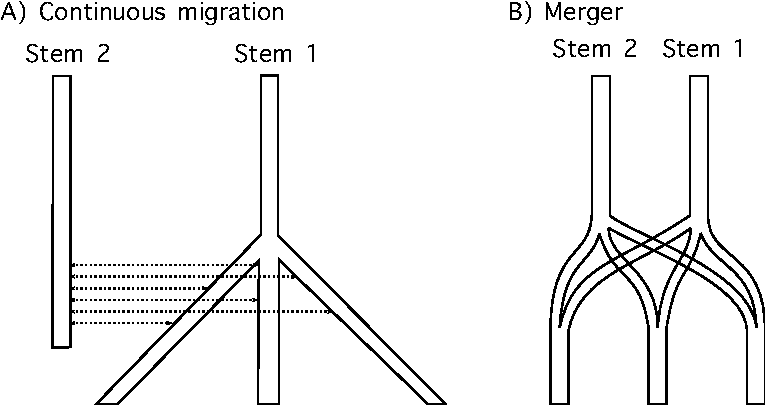
\includegraphics{figures/mergers.pdf}
    \caption{
        \textbf{Two scenarios for population rearrangement.}
        In our demographic models, we considered
        A) continuous migration models, in which one of the stem population expands 
        (splits into contemporary populations), and the other stem population(s)
        has continuous symmetric migration with those populations;
        and B) one or more of the stem populations expands, with instantaneous pulse
        (or ``merger'') events from the other stem population,
        so that recent populations are formed by mergers
        of multiple ancestral populations.
    }
    \label{fig:mergers}
\end{figure}



\begin{figure}[ht]
    \centering
    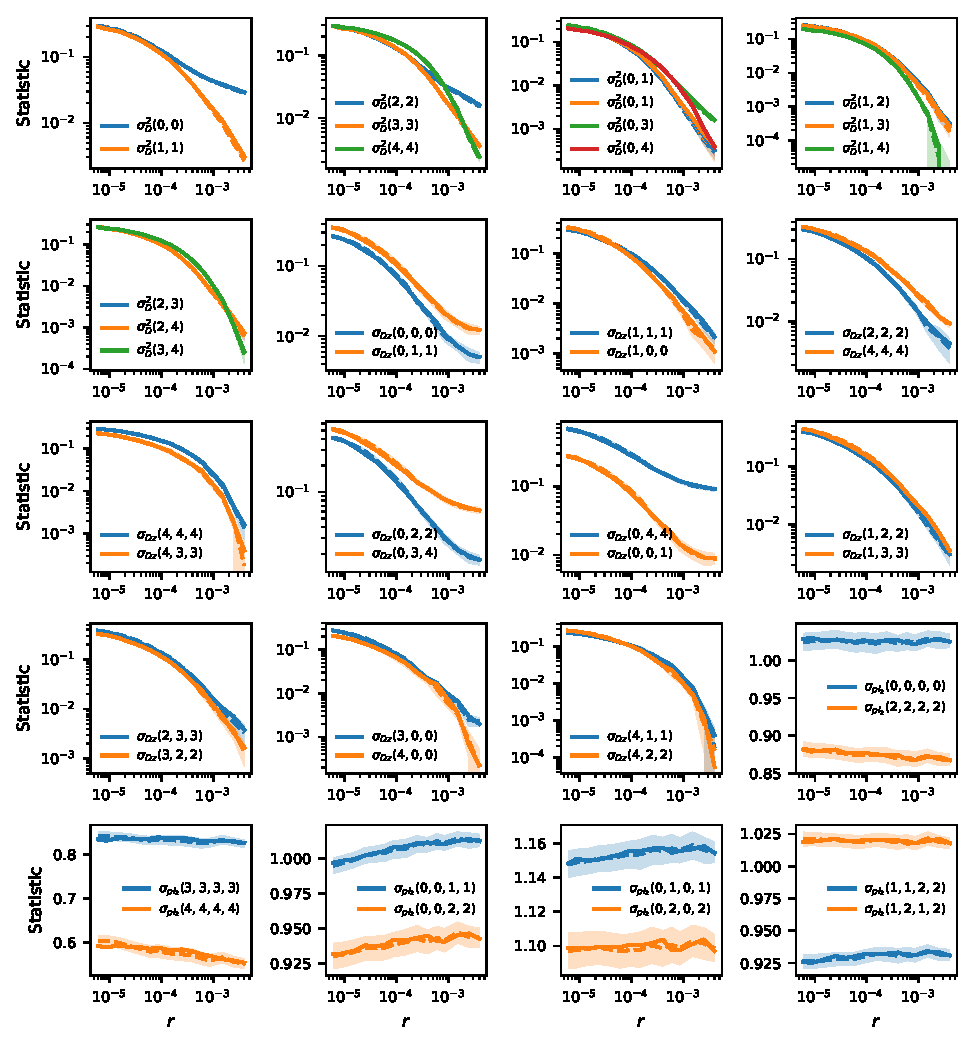
\includegraphics{figures/supp-omni-hapmap-comparison.pdf}
    \caption{
        \textbf{Comparison of LD statistics parsed using two array-based
        recombination maps.}
        The recombination map determines genetic distances between pairs of SNPs,
        so using different maps could result in systematic biases in parsed
        statistics if the maps differ significantly. Here, the solid lines are
        statistics parsed using the HapMapII recombination map, and dashed lines
        are using the OMNI-YRI map. Shading represents 95\% confidence intervals
        from the OMNI map. These two maps results in LD statistics that are
        indistinguishable from one another. Notations for each statistic are
        described in section~\ref{sec:supp-ld-stats} and indexed by populations
        (0: Nama, 1: Mende, 2: Gumuz, 3: Amhara/Oromo, 4: British).
    }
    \label{fig:supp-omni-hapmap-comparison}
\end{figure}

\begin{figure}[ht]
    \centering
    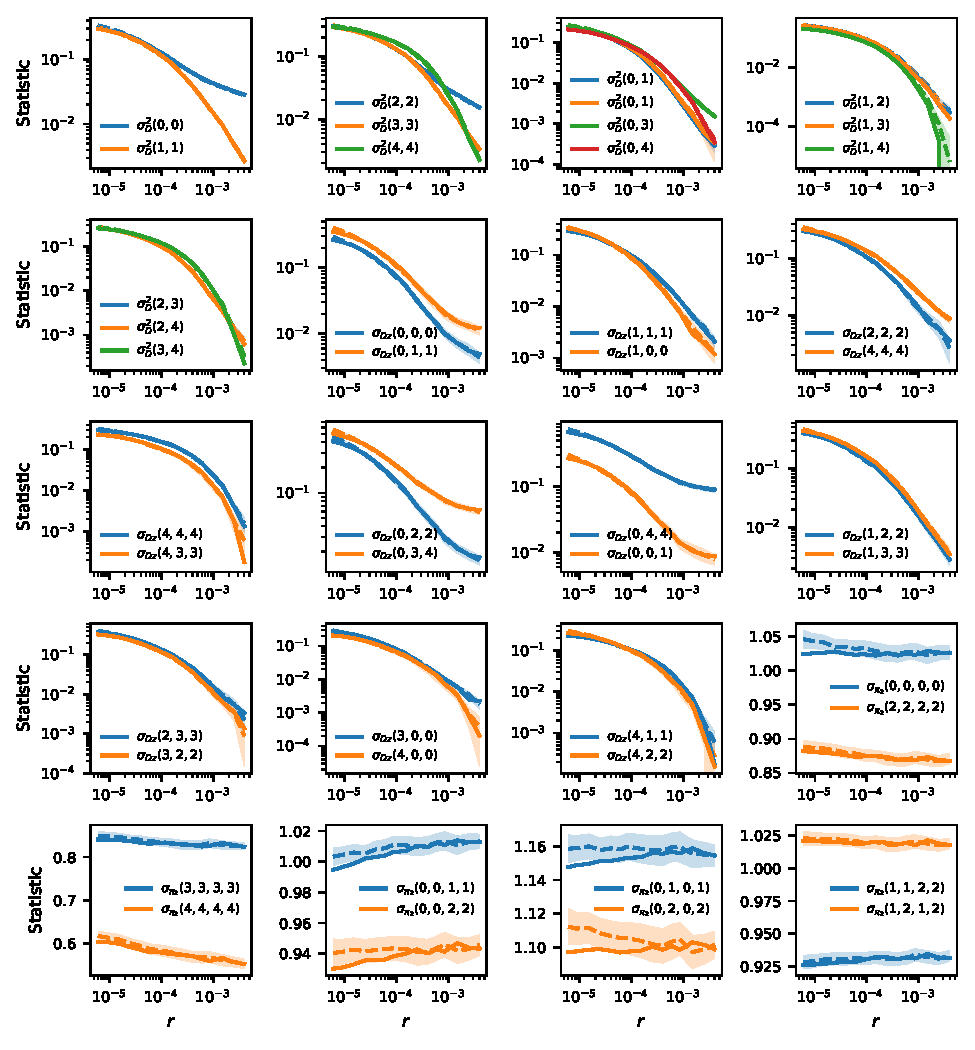
\includegraphics{figures/supp-omni-nama-comparison.pdf}
    \caption{
        \textbf{Comparison of LD statistics parsed using OMNI YRI and
        Nama-specific recombination map.}
        The OMNI YRI recombination map and the Nama-inferred map
        \citep{Van_Eeden2022-od} differ in two primary ways: 1) the YRI and
        Nama have relatively highly diverged ancestries, and 2) the YRI
        map was inferred from low-density array data, while the Nama map
        was inferred from whole-genome sequencing data.
        Nonetheless, LD statistics computed under recombination rates from
        the two maps remain largely concordant, and inferences are
        unaffected by recombination map choice (Section~\ref{sec:supp-results}).
        Shading represents 95\% confidence intervals from the Nama-inferred
        map. Notations for each statistic are described in
        section~\ref{sec:supp-ld-stats}, and indexes represent populations
        (0: Nama, 1: Mende, 2: Gumuz, 3: Amhara/Oromo, 4: British).
    }
    \label{fig:supp-omni-nama-comparison}
\end{figure}

\begin{figure}[ht]
    \centering
    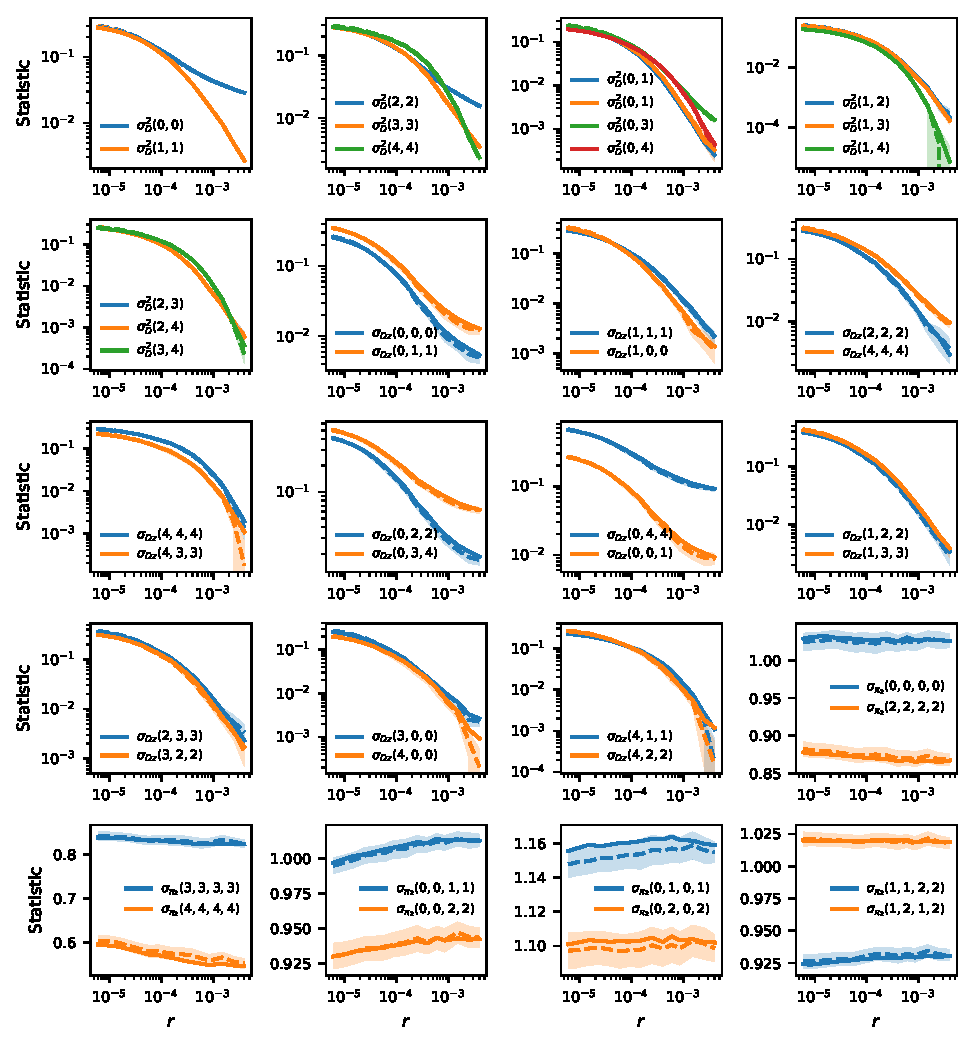
\includegraphics{figures/supp-intergenic-all-snps-comparison.pdf}
    \caption{
        \textbf{Comparison of LD statistics parsed from intergenic loci and
        from all loci across the genome.} Statistics computed from intergenic
        regions (dashed lines, shown with computed standard errors as shaded
        regions) and those computed from all regions genome-wide (solid lines)
        do not show large differences. We chose to perform model inference
        using intergenic regions alone to reduce bias due to selection in and
        around protein-coding regions (Section~\ref{sec:computing-stats}).
        Notations for each statistic are described in
        section~\ref{sec:supp-ld-stats}, and indexes represent populations (0:
        Nama, 1: Mende, 2: Gumuz, 3: Amhara/Oromo, 4: British).
    }
    \label{fig:supp-inter-all-comparison}
\end{figure}

\begin{figure}[ht]
    \centering
    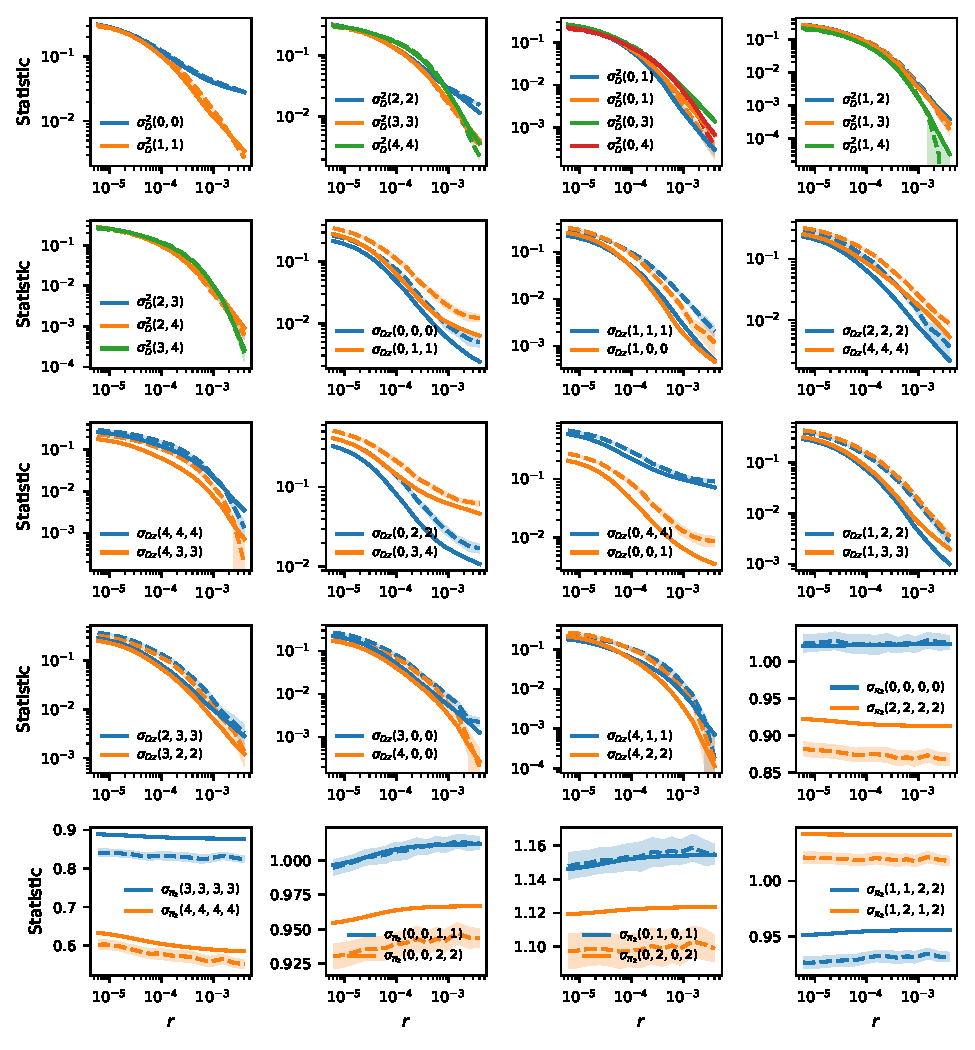
\includegraphics{figures/supp-single-origin-fits.pdf}
    \caption{
        \textbf{Single-origin model fit to LD statistics.}
        Predicted vs observed two-locus statistics as a function of genetic
        distance for the single-origin model. Each panel represents a different
        set of two-locus statistics. Solid lines represent estimates using the
        single-origin model. Dashed lines represent observed statistics.
        Notation and indexing of statistics are described in the
        Fig.~\ref{fig:supp-omni-hapmap-comparison} caption.
    }
    \label{fig:supp-single-origin-fits}
\end{figure}

\begin{figure}[ht]
    \centering
    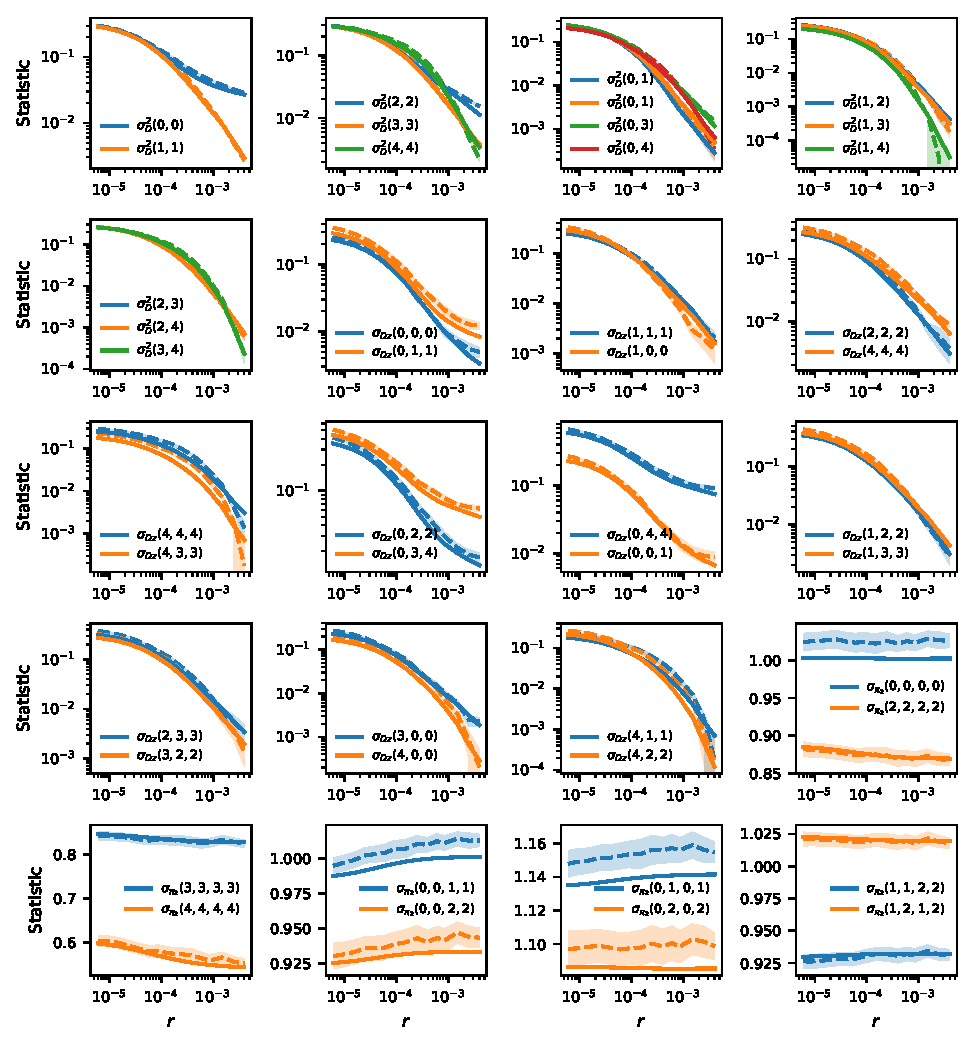
\includegraphics{figures/supp-continuous-migration-fits.pdf}
    \caption{
        \textbf{Continuous-migration model fit to LD statistics.}
        Predicted vs observed two-locus statistics as a function of genetic
        distance for the continuous-migration model with migration between stems.
        Each panel represents a different
        set of two-locus statistics. Solid lines represent estimates using the
        continuous-migration model. Dashed lines represent observed statistics.
        Notation and indexing of statistics are described in the
        Fig.~\ref{fig:supp-omni-hapmap-comparison} caption.
    }
    \label{fig:supp-continuous-migration-fits}
\end{figure}

\begin{figure}[ht]
    \centering
    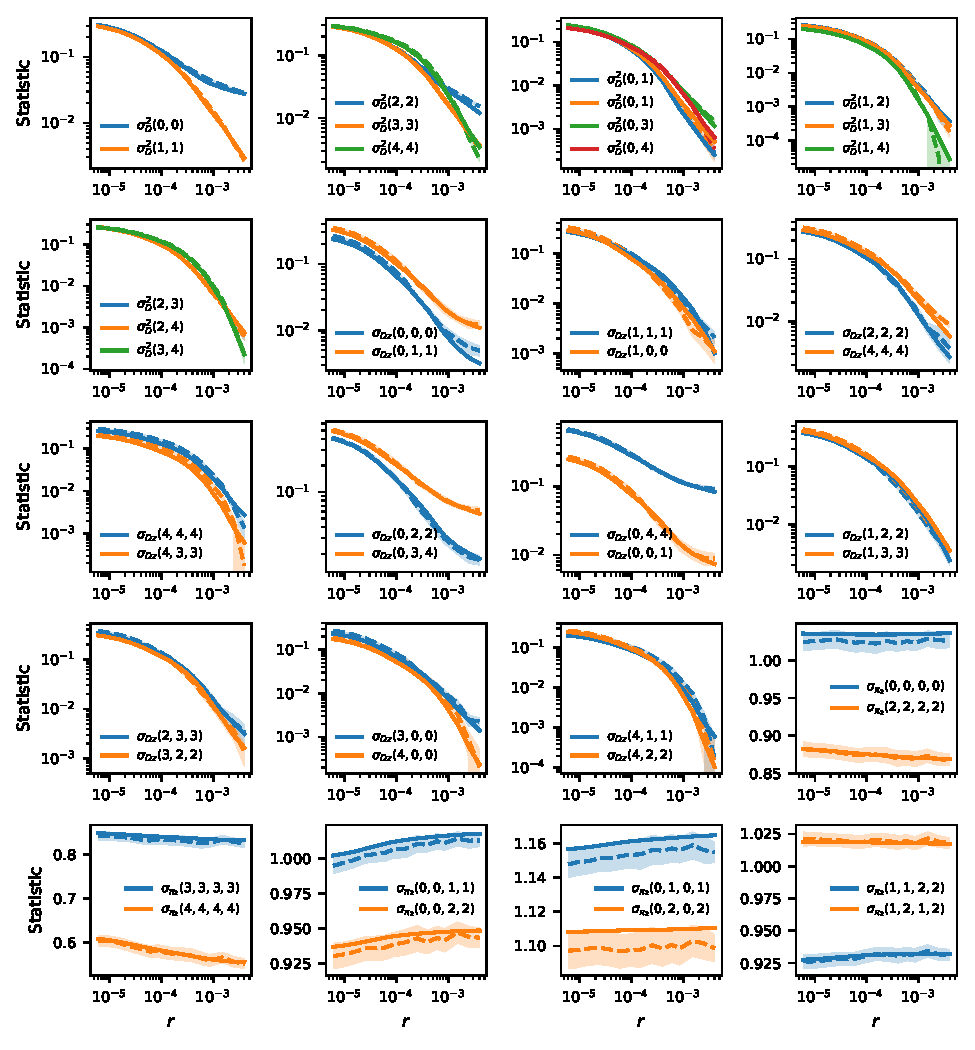
\includegraphics{figures/supp-merger-without-stem-migration-fits.pdf}
    \caption{
        \textbf{Merger-without-stem-migration model fit to LD statistics.}
        Predicted vs observed two-locus statistics as a function of genetic
        distance for the merger-without-stem-migration model. Each panel
        represents a different set of two-locus statistics.
        Solid lines represent estimates using the
        merger-without-stem-migration model.
        Dashed lines represent observed statistics.
        Notation and indexing of statistics are described in the
        Fig.~\ref{fig:supp-omni-hapmap-comparison} caption.
    }
    \label{fig:supp-merger-without-stem-migration-fits}
\end{figure}

\begin{figure}[ht]
    \centering
    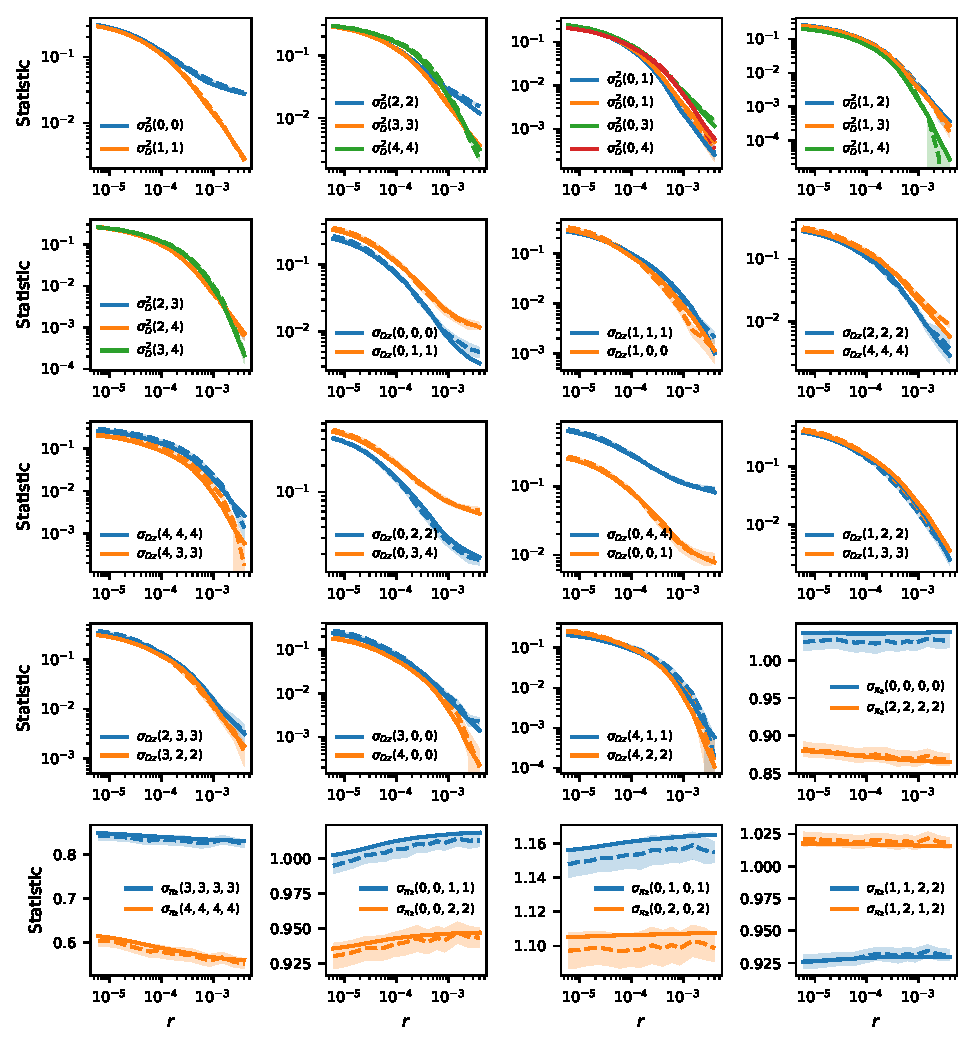
\includegraphics{figures/supp-merger-with-stem-migration-fits.pdf}
    \caption{
        \textbf{Merger-with-stem-migration model fit to LD statistics.}
        Predicted vs observed two-locus statistics as a function of genetic
        distance for the merger-with-stem-migration model. Each panel
        represents a different set of two-locus statistics.
        Solid lines represent estimates using the
        merger-with-stem-migration model.
        Dashed lines represent observed statistics.
        Notation and indexing of statistics are described in the
        Fig.~\ref{fig:supp-omni-hapmap-comparison} caption.
    }
    \label{fig:supp-merger-with-stem-migration-fits}
\end{figure}

\begin{figure}[ht]
    \centering
    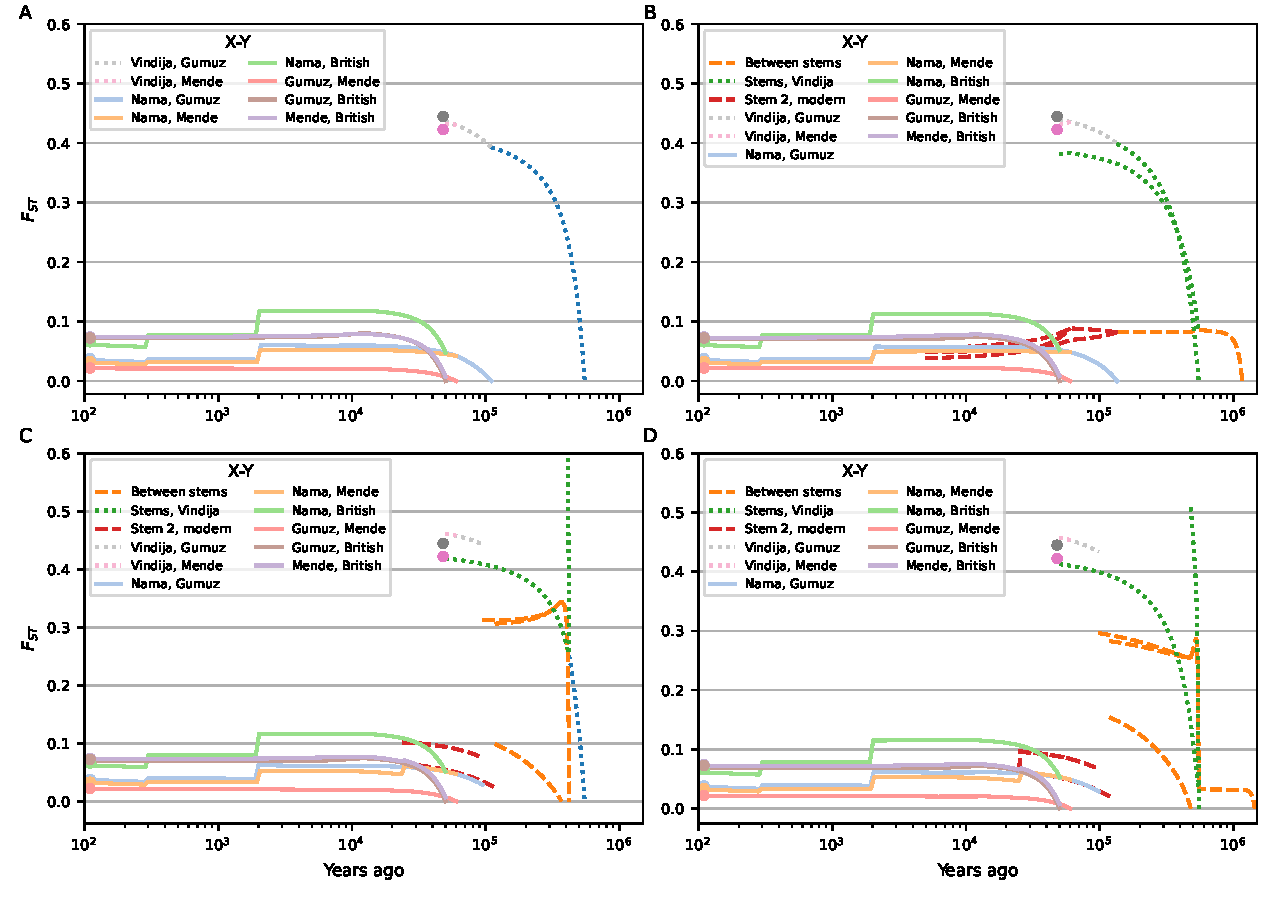
\includegraphics[width=\textwidth]{figures/supp-fsts-all-models.pdf}
    \caption{
        \textbf{Predicted \bm{$F_{ST}$} between contemporaneous populations over time.}
        All models (A: single origin, B: continuous migration, C: merger without stem
        migration, D: merger with stem migration) match observed $F_{ST}$ between
        sampled populations. The continuous-migration model predicts that human stem
        populations remain genetically similar, while the merger with and without
        stem migration models predict a period of increased $F_{ST}$ between ancestors
        of contemporary humans.
        This is largely due to the very small inferred $N_e$ in one of
        the stem branches, which leads to a rapid increase in differentiation due to
        drift.
    }
    \label{fig:supp-FST-panels}
\end{figure}

\begin{figure}[ht]
    \centering
    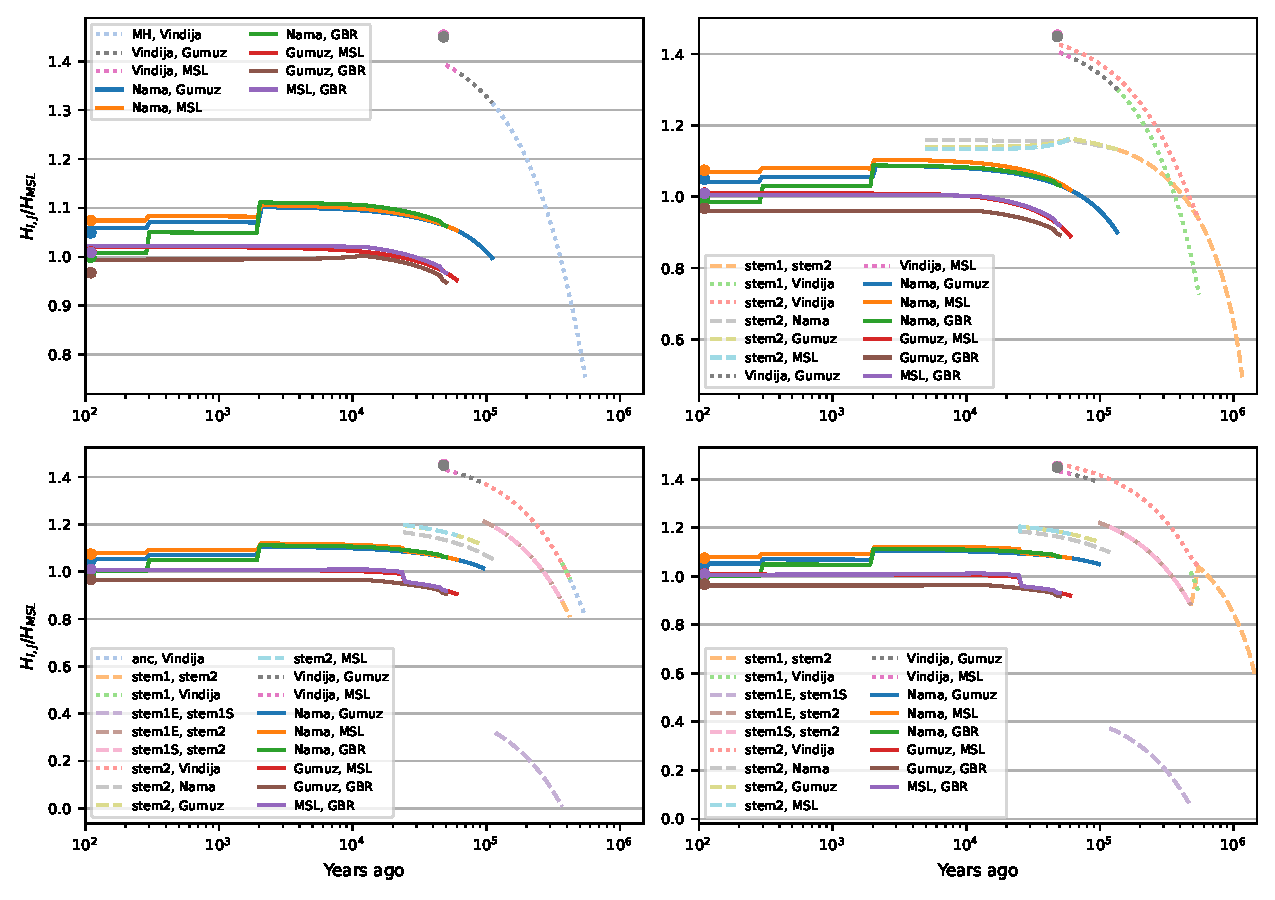
\includegraphics[width=\textwidth]{figures/supp-h12s-all-models.pdf}
    \caption{
        \textbf{Predicted pairwise differentiation between contemporaneous
        populations.} $H_{i,j}$ is the predicted pairwise differentiation
        between two populations per base-pair, using a mutation rate estimated
        from matching predicted to observed pairwise diversity from the
        intergenic data used in the fits (see Sec.~\ref{sec:supp-mutation}).
        The single-origin model (A) shows larger deviations between observed
        and expected differentiation than the models with early human structure
        (B: continuous migration, C: merger without stem migration, D: merger
        with stem migration). In the merger models (C and D), while $F_{ST}$ is
        large between early stems due to the sharp bottleneck in one of those
        branches, the pairwise differences are comparable to the
        continuous-migration model. Stem 1E and Stem 1S have low
        differentiation, as the bottleneck in Stem 1 (which they both split
        from) sharply reduces diversity by the time of the split. This has the
        effect of large $F_{ST}$ but small $H_{i,j}$.
    }
    \label{fig:supp-h12-panels}
\end{figure}

\begin{figure}[ht]
    \centering
    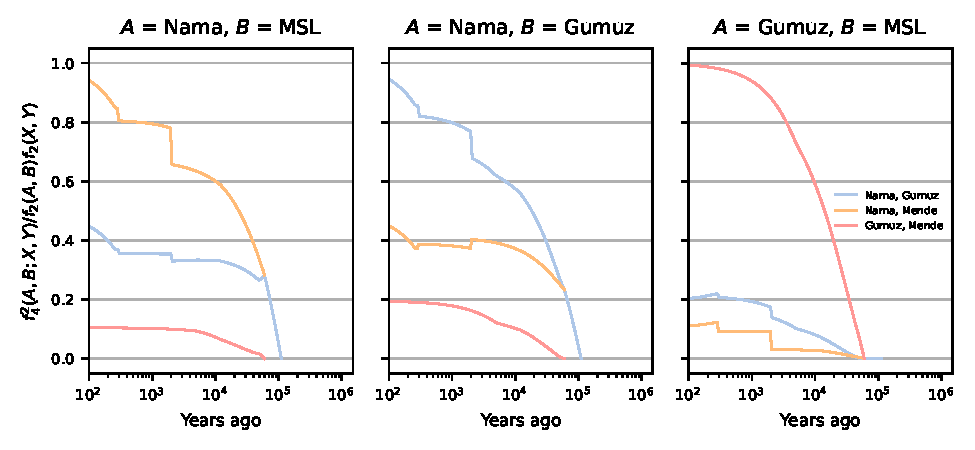
\includegraphics{figures/supp-f4s-single-origin.pdf}
    \caption{
        \textbf{Predicted \bm{$f_4$} between pairs of contemporary human populations
        and ancient branches from the single-origin model.}
        $f_4^2(A, B; X, Y)/f_2(A, B)f_2(X, Y)$ is interpreted as the proportion of the
        amount of drift between sampled populations $A$ and $B$ that aligns with
        drift between populations $X$ and $Y$, sampled in the past
        (see Section~\ref{sec:f4}). In the single-origin model, nearly all
        differentiation between the Nama, Mende, and Gumuz populations arises
        after the divergence events, so normalized $f_4$ decays to zero by the
        time of those divergences.
    }
    \label{fig:supp-f4s-single-origin}
\end{figure}

\begin{figure}[ht]
    \centering
    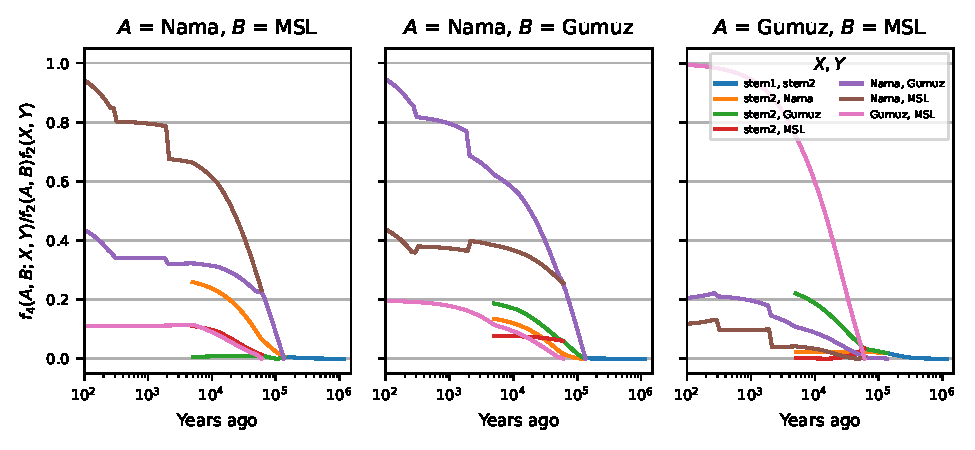
\includegraphics{figures/supp-f4s-continuous-migration.pdf}
    \caption{
        \textbf{Predicted \bm{$f_4$} between pairs of contemporary human populations
        and ancient branches from the continuous-migration model.} 
        $f_4^2(A, B; X, Y)/f_2(A, B)f_2(X, Y)$ is interpreted as the proportion of the
        amount of drift between sampled populations $A$ and $B$ that aligns with
        drift between populations $X$ and $Y$, sampled in the past
        (see Section~\ref{sec:f4}).
        Despite population structure inferred to have extended up to 1Ma
        into the past, differentiation between contemporary African populations
        only traces back to differentiation between ancestral populations
        $\sim$100-200ka, indicating that while stem populations were structured
        (Fig.~\ref{fig:supp-FST-panels}), differentiation due to that
        ancient structure contributes little to differentiation between contemporary
        populations.
    }
    \label{fig:supp-f4s-continuous-migration}
\end{figure}

\begin{figure}[ht]
    \centering
    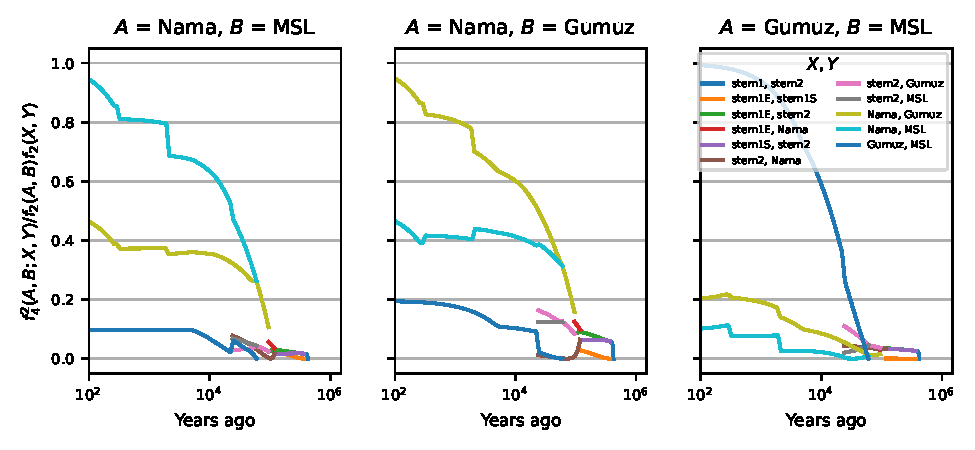
\includegraphics{figures/supp-f4s-merger-without-stem-migration.pdf}
    \caption{
        \textbf{Predicted \bm{$f_4$} between pairs of contemporary human populations
        and ancient branches from the merger-without-stem-migration model.}
        $f_4^2(A, B; X, Y)/f_2(A, B)f_2(X, Y)$ is interpreted as the proportion of the
        amount of drift between sampled populations $A$ and $B$ that aligns with
        drift between populations $X$ and $Y$, sampled in the past
        (see Section~\ref{sec:f4}).
        Unlike the continuous-migration model, population structure in the stems
        following the divergence of Neanderthal and human ancestors results
        in differentiation among contemporary populations that aligns with drift
        between the stems. In this model, migration between stem populations
        is disallowed.
    }
    \label{fig:supp-f4s-merger-without-stem-migration}
\end{figure}

\begin{figure}[ht]
    \centering
    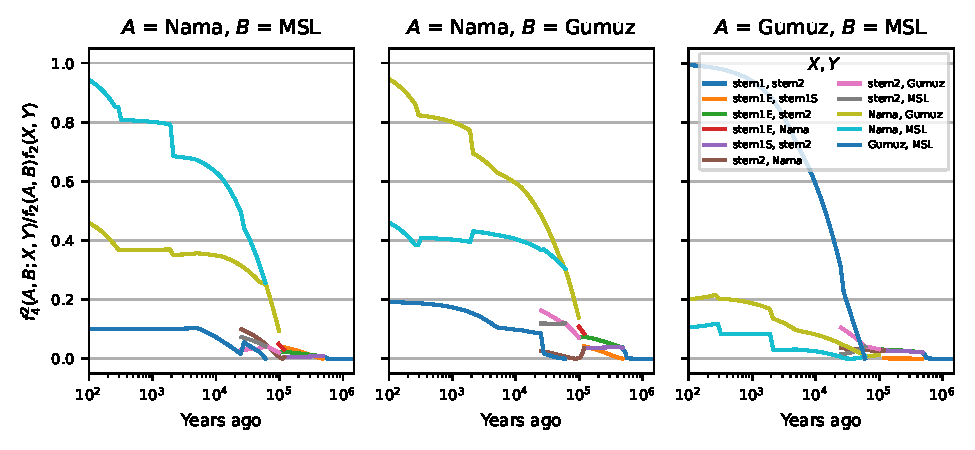
\includegraphics{figures/supp-f4s-merger-with-stem-migration.pdf}
    \caption{
        \textbf{Predicted \bm{$f_4$} between pairs of contemporary populations
        and ancient branches from the merger-with-stem-migration model.}
        $f_4^2(A, B; X, Y)/f_2(A, B)f_2(X, Y)$ is interpreted as the proportion of the
        amount of drift between sampled populations $A$ and $B$ that aligns with
        drift between populations $X$ and $Y$, sampled in the past
        (see Section~\ref{sec:f4}).
        Differentiation between present-day populations aligns with
        up to $\approx 5\%$ of the drift between stems, although some
        population pairs show even less shared drift.
    }
    \label{fig:supp-f4s-merger-with-stem-migration}
\end{figure}

\begin{figure}[ht]
    \centering
    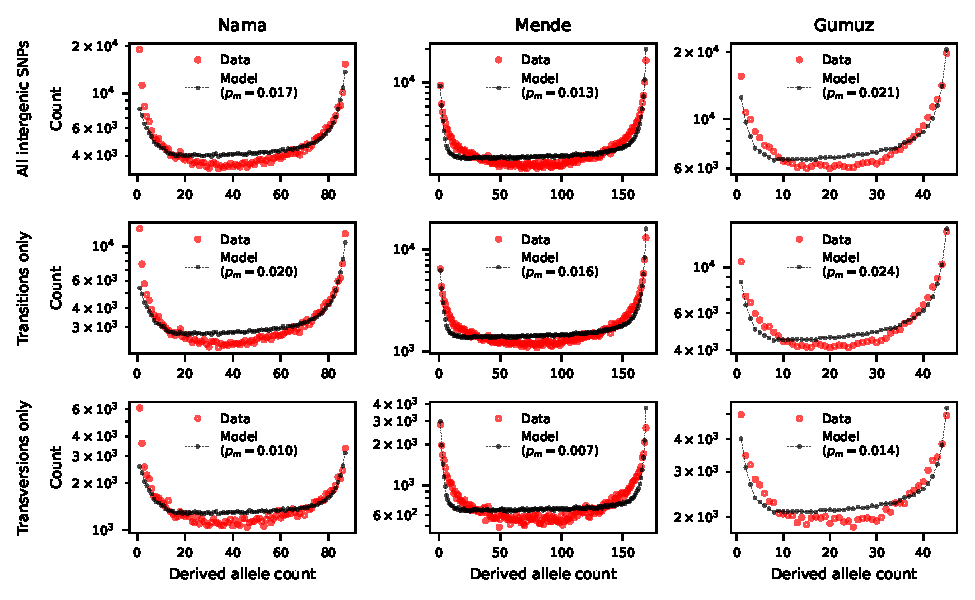
\includegraphics{figures/supp-csfs-single-origin.pdf}
    \caption{
        \textbf{Conditional SFS compared to single-origin model predictions.}
        The single-origin model provides a poor fit to the Neanderthal-conditional SFS in
        the Mende, Gumuz, and Nama (see Section \ref{sec:cSFS}). Ancestral state misidentification
        (labeled as $p_m$ in the figure legends) was
        inferred to be between 1 and $2\%$, and misidentification rates were
        consistent across model comparisons. Misidentification rates of
        transition-type mutations were roughly double that of transversion-type
        mutations, consistent with the higher mutation rates of transition
        mutations vs. transversions.
    }
    \label{fig:supp-csfs-single-origin}
\end{figure}

\begin{figure}[ht]
    \centering
    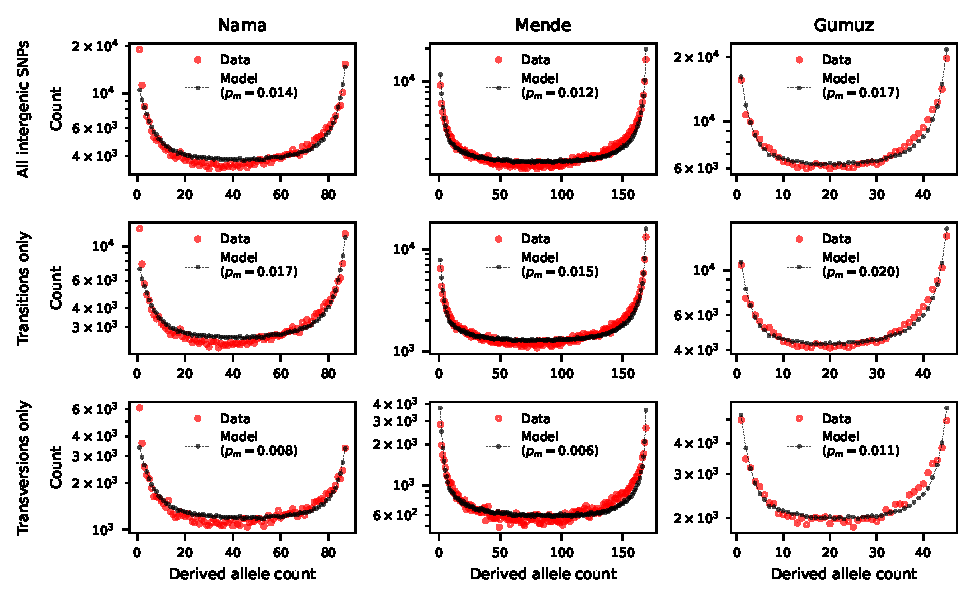
\includegraphics{figures/supp-csfs-continuous-migration.pdf}
    \caption{
        \textbf{Conditional SFS compared to continuous-migration model predictions.}
        The continuous-migration model provides a better fit to the
        Neanderthal-conditional SFS than
        either the single-origin model or the merger-without-stem-migration
        model, although systematic deviations are still noticeable in each
        population. Ancestral state misidentification ($p_m$), as estimated
        with all models, is roughly doubled for transition-type mutations
        compared to transversions.
    }
    \label{fig:supp-csfs-continuous-migration}
\end{figure}

\begin{figure}[ht]
    \centering
    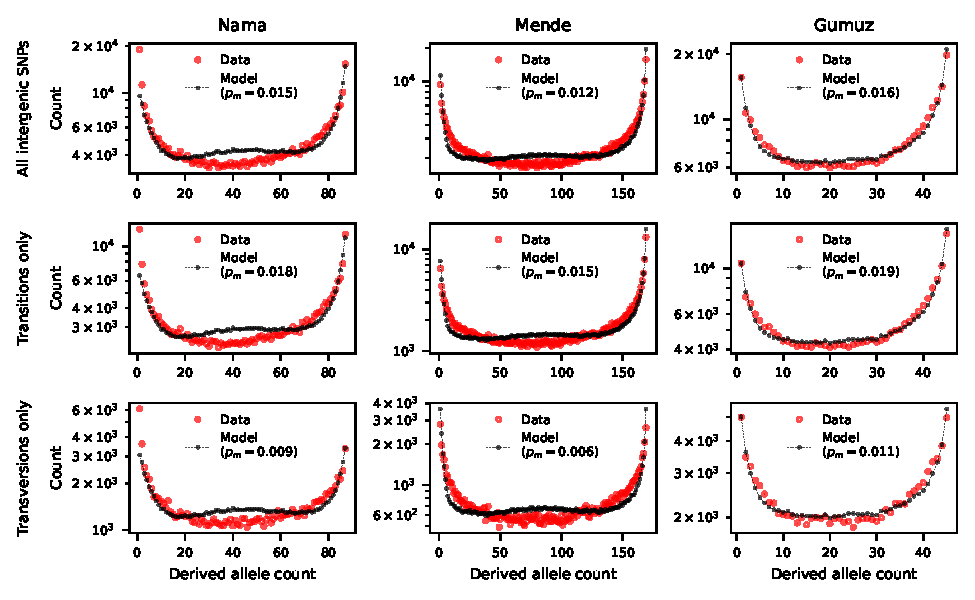
\includegraphics{figures/supp-csfs-merger-without-stem-migration.pdf}
    \caption{
        \textbf{Conditional SFS compared to merger-without-stem-migration model predictions.}
        The excess of intermediate-frequency variants in the Nama and Mende
        cSFS results in a poorer fit to the cSFS compared to the continuous-migration
        and merger-with-stem-migration models. Thus the model without stem migrations
        provides a poorer fit 
        to both two-locus statistics and the cSFS.
        Ancestral state misidentification for transition-type mutations ($p_m$), as estimated
        with all models, is roughly double that of transversions.
    }
    \label{fig:supp-csfs-merger-without-stem-migration}
\end{figure}

\begin{figure}[ht]
    \centering
    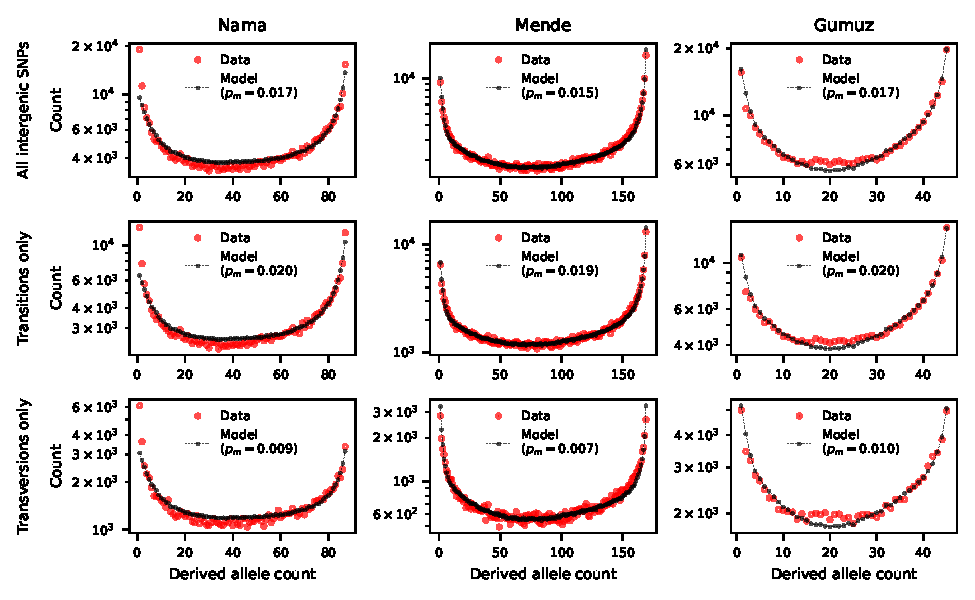
\includegraphics{figures/supp-csfs-merger-with-stem-migration.pdf}
    \caption{
        \textbf{Conditional SFS compared to merger-with-stem-migration model predictions.}
        The merger-with-stem-migration model, in addition to providing the best
        fit to heterozygosity and LD statistics, provided the best fit to the cSFS
        in the Nama, Gumuz, and Mende populations. Rates of ancestral state
        misidentification were consistent across each comparison, with the
        ancestral state of transversion mutations estimated to be $0.7-1.0\%$, and
        that of transition mutations estimated to be $1.9-2.0\%$. These
        misidentification rates are consistent with the known difference in mutation
        rates between transitions and transversions, as well as other SFS-based
        inferences in humans using the Thousand Genomes data and the 6-primate
        alignment (see Methods). 
    }
    \label{fig:supp-csfs-merger-with-stem-migration}
\end{figure}

\begin{figure}[ht]
    \centering
    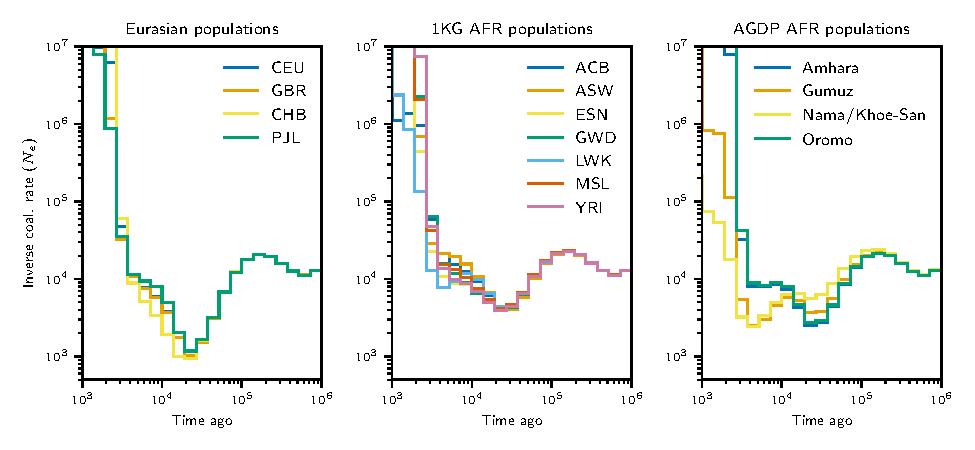
\includegraphics{figures/supp-relate-iicr-data}
    \caption{
        \textbf{Inverse instantaneous coalescence rates inferred from the data.}
        Using combined data from the Thousand Genomes Project and the ADRP,
        we reconstructed gene genealogies using Relate and calculated the
        inverse instantaneous coalescence rate for samples within each population.
        (A) Eurasian populations (CEU: European American, GBR: British,
        CHB: Han Chinese, PJL: Punjabi), (B) Thousand Genomes African populations
        (ACB: Afro-Caribbean, ASW: African American, ESN: Esan, GWD: Gambian,
        LWK: Luhya, MSL: Mende, YRI: Yoruba), (C) ADRP populations.
    }
    \label{fig:supp-iicr-data}
\end{figure}

\begin{figure}[ht]
    \centering
    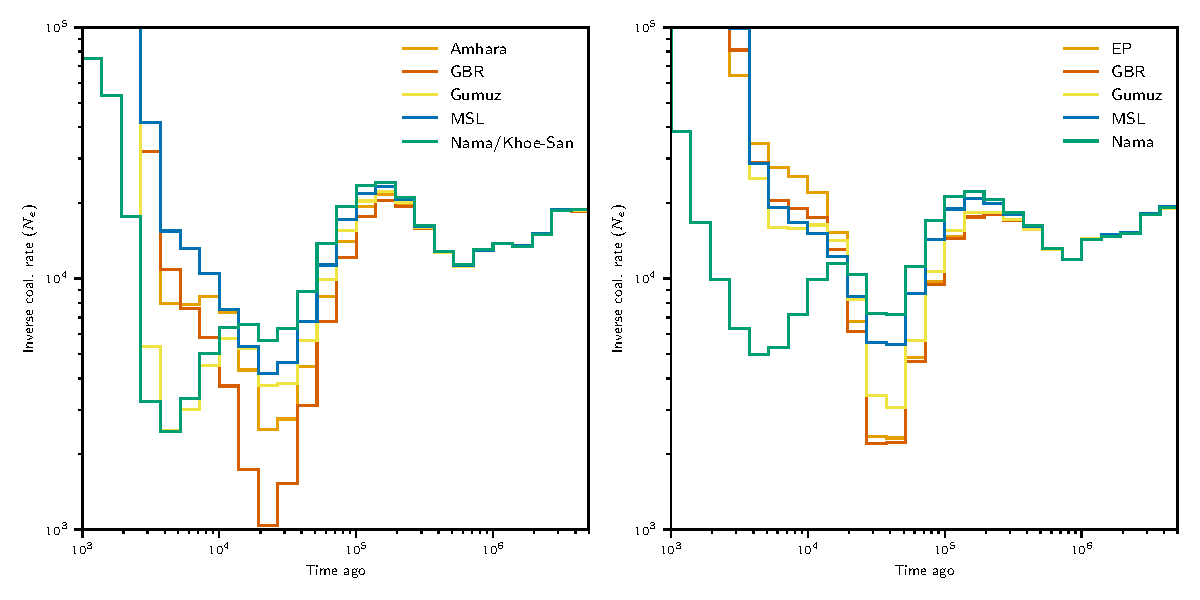
\includegraphics[width=\textwidth]{figures/supp-relate-iicr-data-full-and-subset}
    \caption{
        \textbf{Inverse instantaneous coalescence rates inferred from the data,
        subset to focal populations in the model inferences.}
        Fig.~\ref{fig:supp-iicr-data} shows IICR curves from reconstructed
        genealogies inferred using a larger dataset (including nearly 1,200
        individuals) than the subset of populations we primarily focused on
        here. To assess the robustness of Relate-inferred genealogies and for a
        direct comparison to our inferred demographic models, we ran Relate on
        the 290 genomes from the Nama, Gumuz, Mende, Amhara/Oromo, and British individuals.
        While the reconstructed IICR curves are qualitatively similar to those
        from the full dataset for these populations in the distant past, there
        are noticeable discrepancies over the recent history in the last tens of
        thousands of years. Left: Relate run on full dataset, showing focal
        populations. Right: Relate run directly on the subset dataset of focal
        populations.
    }
    \label{fig:supp-iicr-data-subset}
\end{figure}

\begin{figure}[ht]
    \centering
    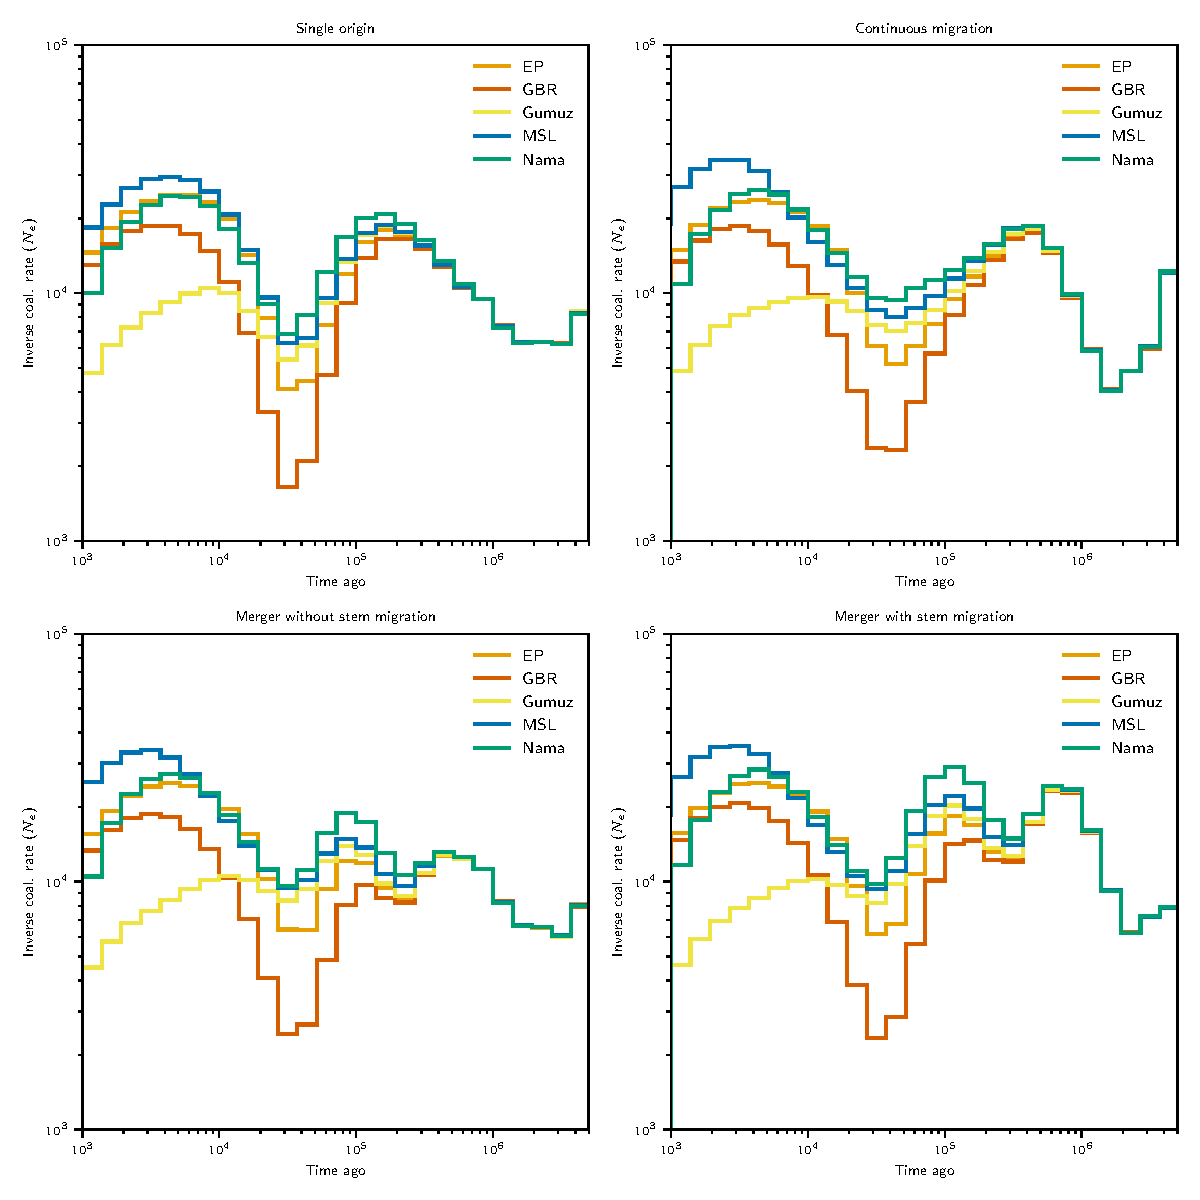
\includegraphics[width=\textwidth]{figures/supp-relate-iicr-simulation}
    \caption{
        \textbf{Inverse instantaneous coalescence rates reinferred from
        simulated data.} We simulated data under our four highlighted models,
        sampling the same number of individuals per population as the original
        dataset, and then ran Relate on each simulated dataset to reconstruct
        IICR curves for each. Each model has qualitatively different histories,
        particularly for the distant past with varying numbers and timings of
        oscillations. However, due to the discrepancies in reconstructed
        genealogies using even the same data as input
        (Figs.~\ref{fig:supp-iicr-data-subset} and \ref{fig:supp-rccr-data}),
        it is difficult to draw firm conclusions from quantitative comparisons
        between reconstructed genealogies.
    }
    \label{fig:supp-iicr-sim}
\end{figure}

\begin{figure}[ht]
    \centering
    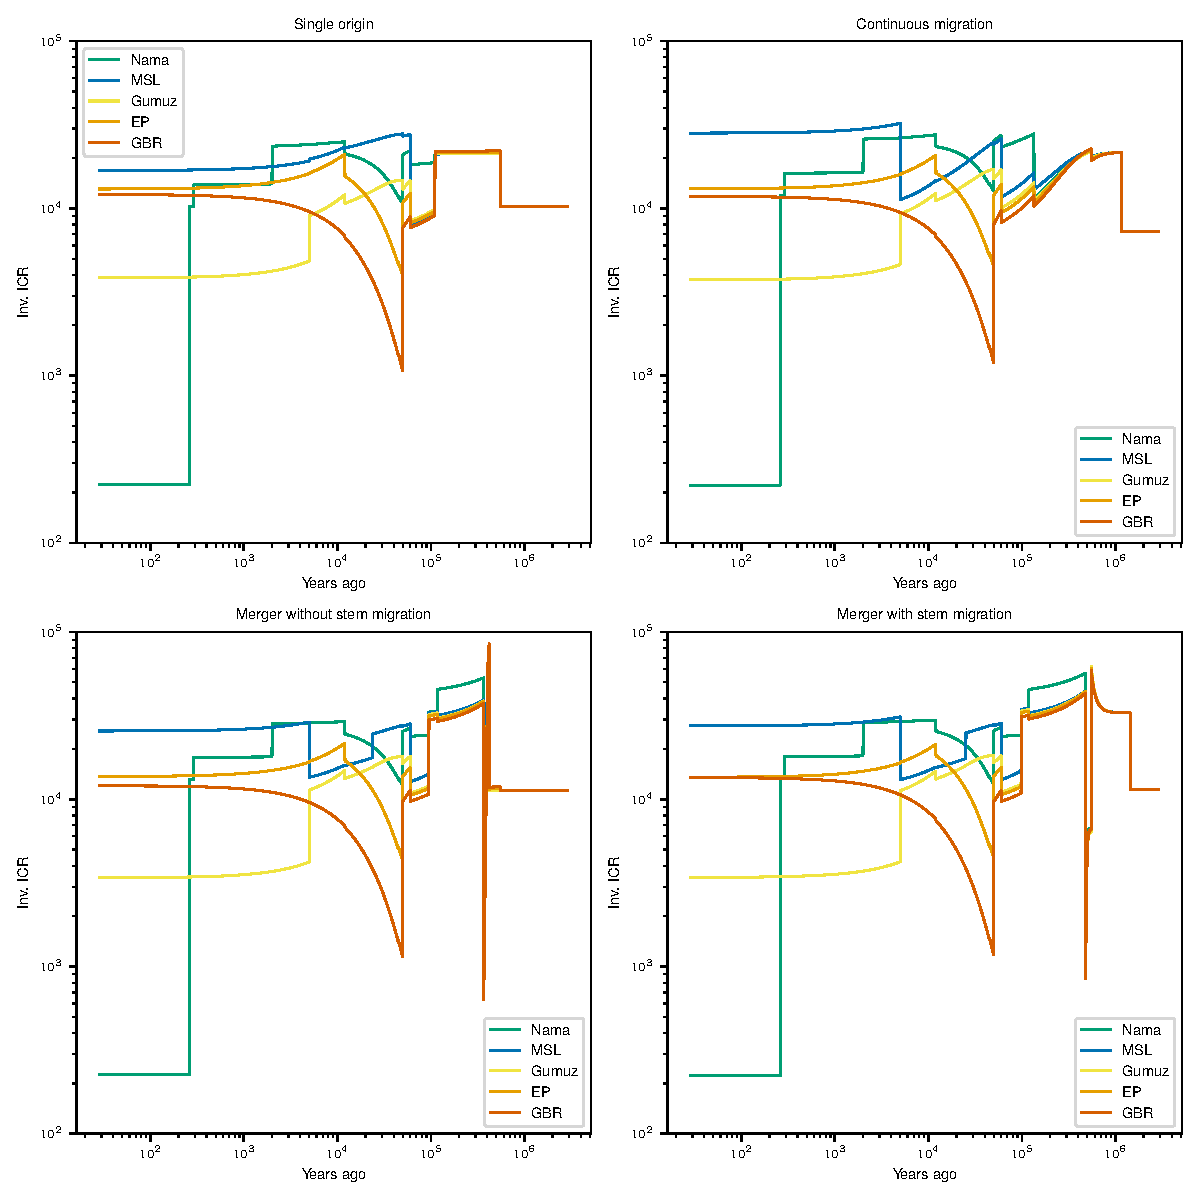
\includegraphics[width=\textwidth]{figures/supp-exp-coal-rates}
    \caption{
        \textbf{Expected inverse instantaneous coalescence rates from models.}
        The inferred demographic models specify population sizes, split times,
        and migration rates and events, making it possible to compute the exact
        expected IICR curve for each population. Due to discrete events
        (instantaneous size changes, for example), the models can produce
        non-smooth IICR curves, although each predicts a period of increased
        ``effective size'' in the past $\sim200-500$ka.
    }
    \label{fig:supp-iicr-exp}
\end{figure}

\begin{figure}[ht]
    \centering
    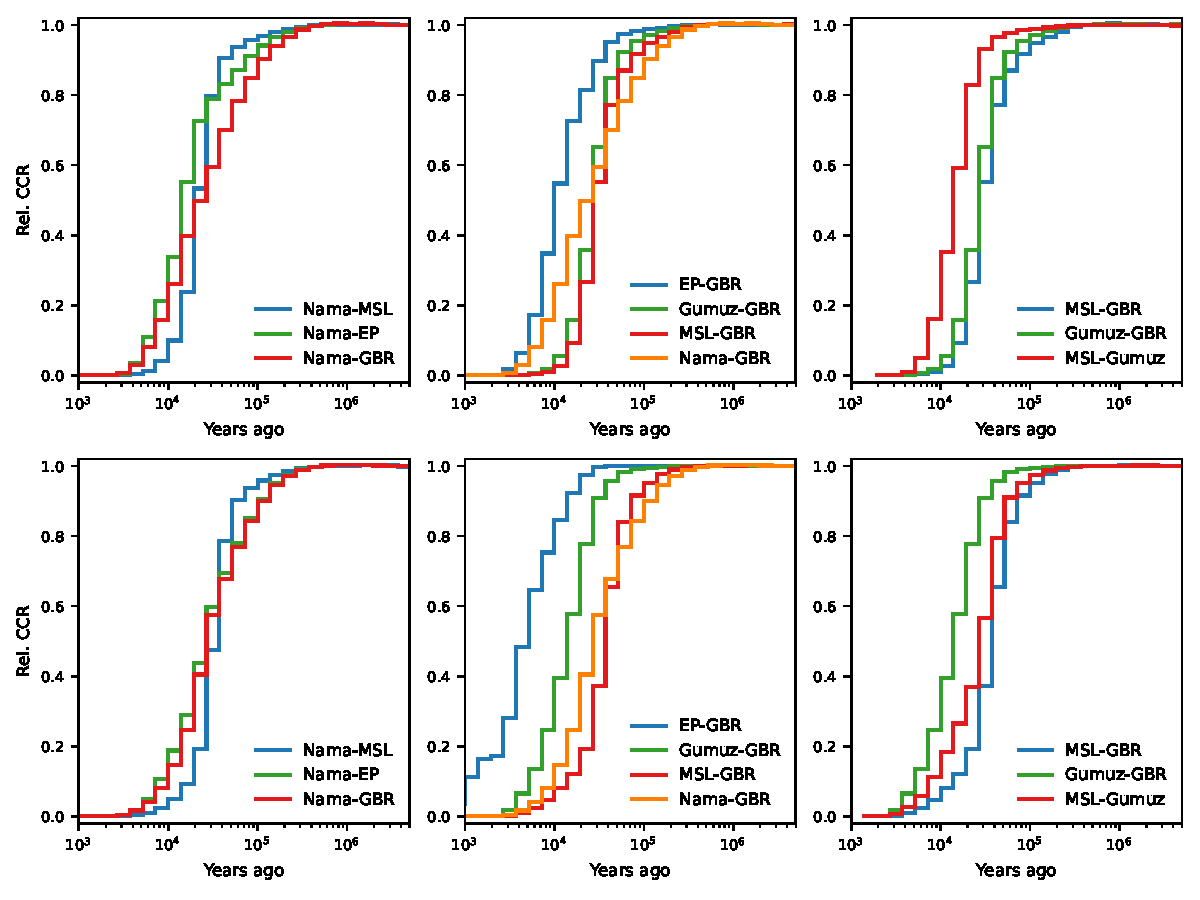
\includegraphics[width=\textwidth]{figures/supp-relate-rccr-data-full-and-subset}
    \caption{
        \textbf{Relative cross-coalescence rates inferred from the data.} Using
        the same reconstructed genealogies from Relate as displayed in
        Fig.~\ref{fig:supp-iicr-data-subset}, 
        we computed relative cross-coalescence (RCCR) curves
        for pairs of populations using genealogies from the either the full dataset
        ($\sim1,200$ individuals, top) and the subset of focal populations (290
        individuals, bottom). Despite the overlap in samples, the two sets of inferred
        genealogies provided inconsistent RCCR, with both the timing and
        ordering of increased RCCR varying between the two datasets.
        Genealogies reconstructed from the full dataset provide a better match
        to each of inferred demographic models
        (Figs.~\ref{fig:supp-rccr-single-origin}--\ref{fig:supp-rccr-merger-with-stem-migration}).
    }
    \label{fig:supp-rccr-data}
\end{figure}

\begin{figure}[ht]
    \centering
    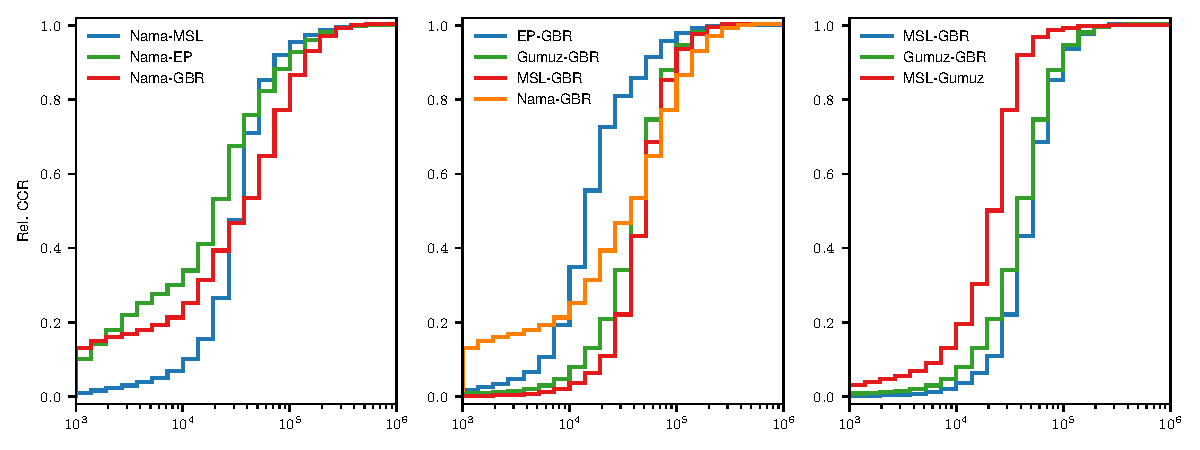
\includegraphics[width=\textwidth]{figures/supp-relate-rccr-single-origin}
    \caption{
        \textbf{Relative cross-coalescence rates reinferred from simulated data
        under the single-origin model.} RCCR curves from genealogies
        reconstructed from simulated data using Relate match those inferred
        from the full dataset (\ref{fig:supp-rccr-data}, top) for distant
        time points. There are large discrepancies in the very recent history,
        where Relate and other genome-wide coalescence-based methods are known
        to be underpowered.
    }
    \label{fig:supp-rccr-single-origin}
\end{figure}

\begin{figure}[ht]
    \centering
    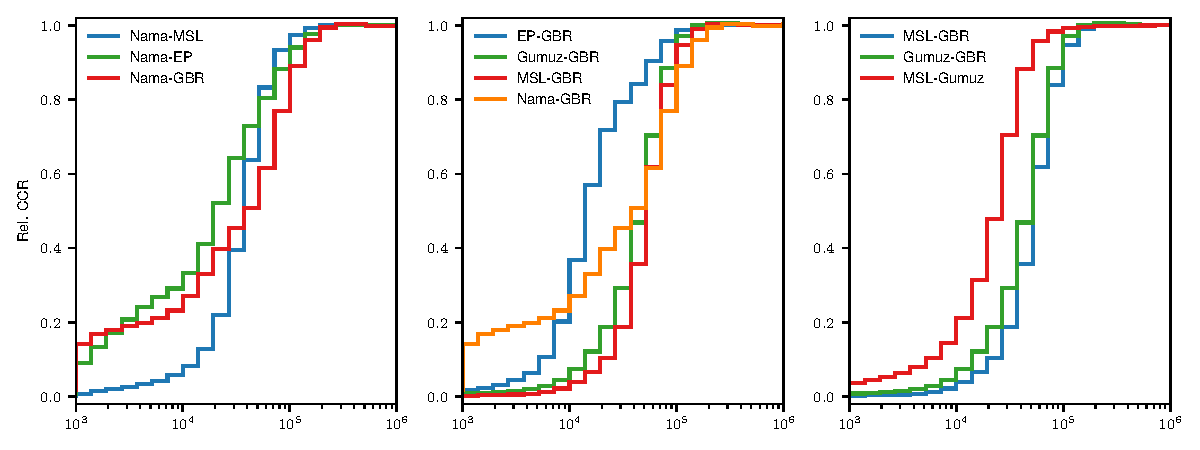
\includegraphics[width=\textwidth]{figures/supp-relate-rccr-continuous-migration}
    \caption{
        \textbf{Relative cross-coalescence rates reinferred from simulated data
        under the continuous-migration model.} RCCR curves from genealogies
        reconstructed from simulated data using Relate match those inferred
        from the full dataset (\ref{fig:supp-rccr-data}, top) for distant
        time points. There are large discrepancies in the very recent history,
        where Relate and other genome-wide coalescence-based methods are known
        to be underpowered.
    }
    \label{fig:supp-rccr-continuous-migration}
\end{figure}

\begin{figure}[ht]
    \centering
    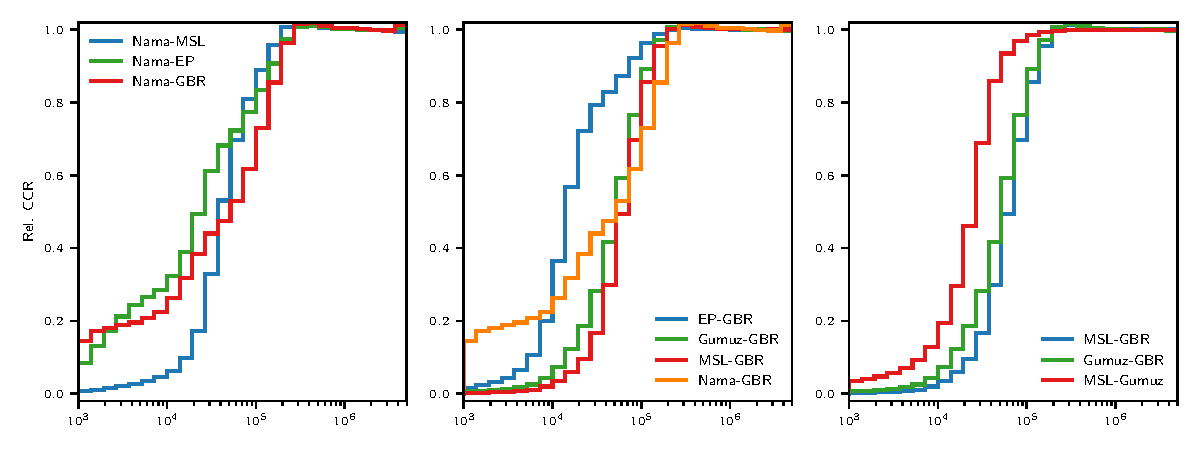
\includegraphics[width=\textwidth]{figures/supp-relate-rccr-merger-without-stem-migration}
    \caption{
        \textbf{Relative cross-coalescence rates reinferred from simulated data
        under the merger-without-stem-migration-model.} RCCR curves from genealogies
        reconstructed from simulated data using Relate match those inferred
        from the full dataset (\ref{fig:supp-rccr-data}, top) for distant
        time points. There are large discrepancies in the very recent history,
        where Relate and other genome-wide coalescence-based methods are known
        to be underpowered.
    }
    \label{fig:supp-rccr-merger-without-stem-migration}
\end{figure}

\begin{figure}[ht]
    \centering
    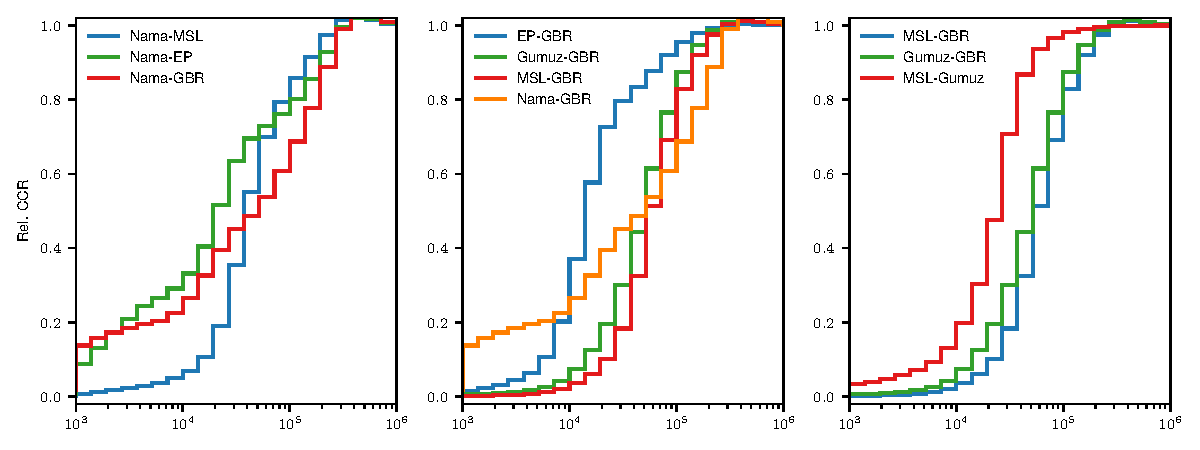
\includegraphics[width=\textwidth]{figures/supp-relate-rccr-merger-with-stem-migration}
    \caption{
        \textbf{Relative cross-coalescence rates reinferred from simulated data
        under the merger-with-stem-migration model.} RCCR curves from genealogies
        reconstructed from simulated data using Relate match those inferred
        from the full dataset (\ref{fig:supp-rccr-data}, top) for distant
        time points. There are large discrepancies in the very recent history,
        where Relate and other genome-wide coalescence-based methods are known
        to be underpowered.
    }
    \label{fig:supp-rccr-merger-with-stem-migration}
\end{figure}

\begin{figure}[ht]
    \centering
    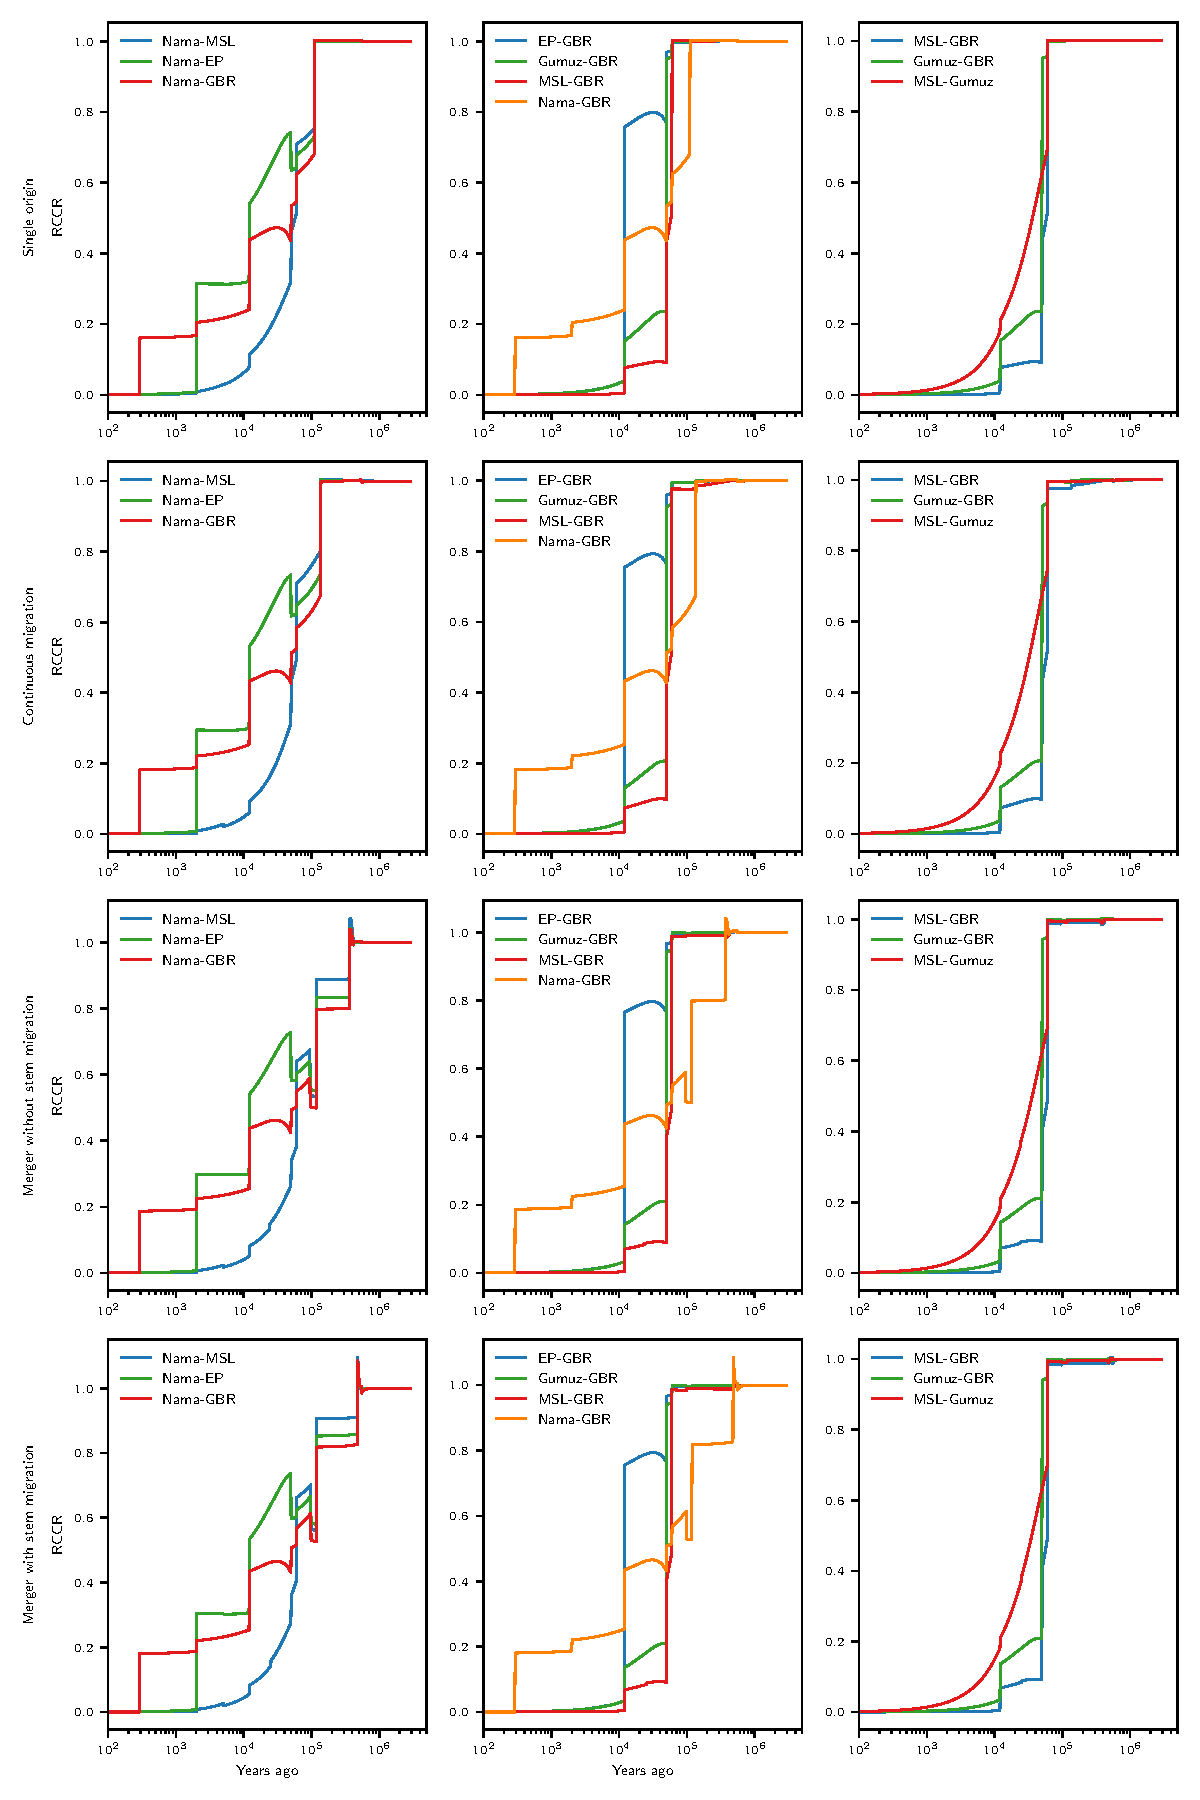
\includegraphics[width=0.75\textwidth]{figures/supp-relate-rccr-model-exp.pdf}
    \caption{
        \textbf{Expected relative cross-coalescence rates from inferred models.}
        Our inferred demographic models allow for exact calculation of expected
        RCCR curves, showing that while the parameterizations of the four models
        are quite different, they each predict very similar RCCR profiles.
    }
    \label{fig:supp-rccr-exp}
\end{figure}

\begin{figure}[ht]
    \centering
    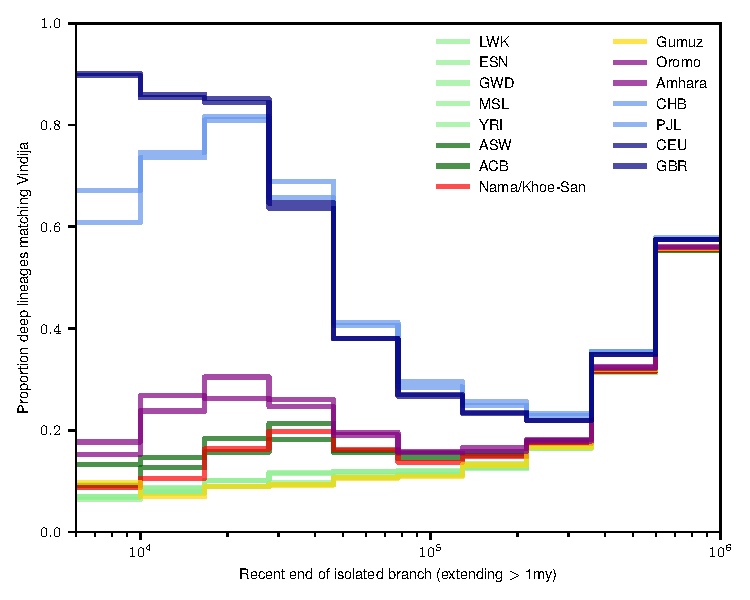
\includegraphics{figures/supp-deep-brances-data}
    \caption{
        \textbf{Neanderthal-matching deep branch distribution from the data.}
        Following the approach of \citet{Speidel2019-nj}, we categorized
        Neanderthal-matching deep branches for each population from
        Relate-inferred gene genealogies. The proportion of deep branches with
        Neanderthal affinity is highest for Eurasian populations, as expected,
        and higher for African populations with recent Eurasian ancestry
        (Oromo, Amhara, ACB, ASW, and Nama) than the Gumuz and West African
        populations. 
    }
    \label{fig:supp-deep-branches}
\end{figure}

\begin{figure}[ht]
    \centering
    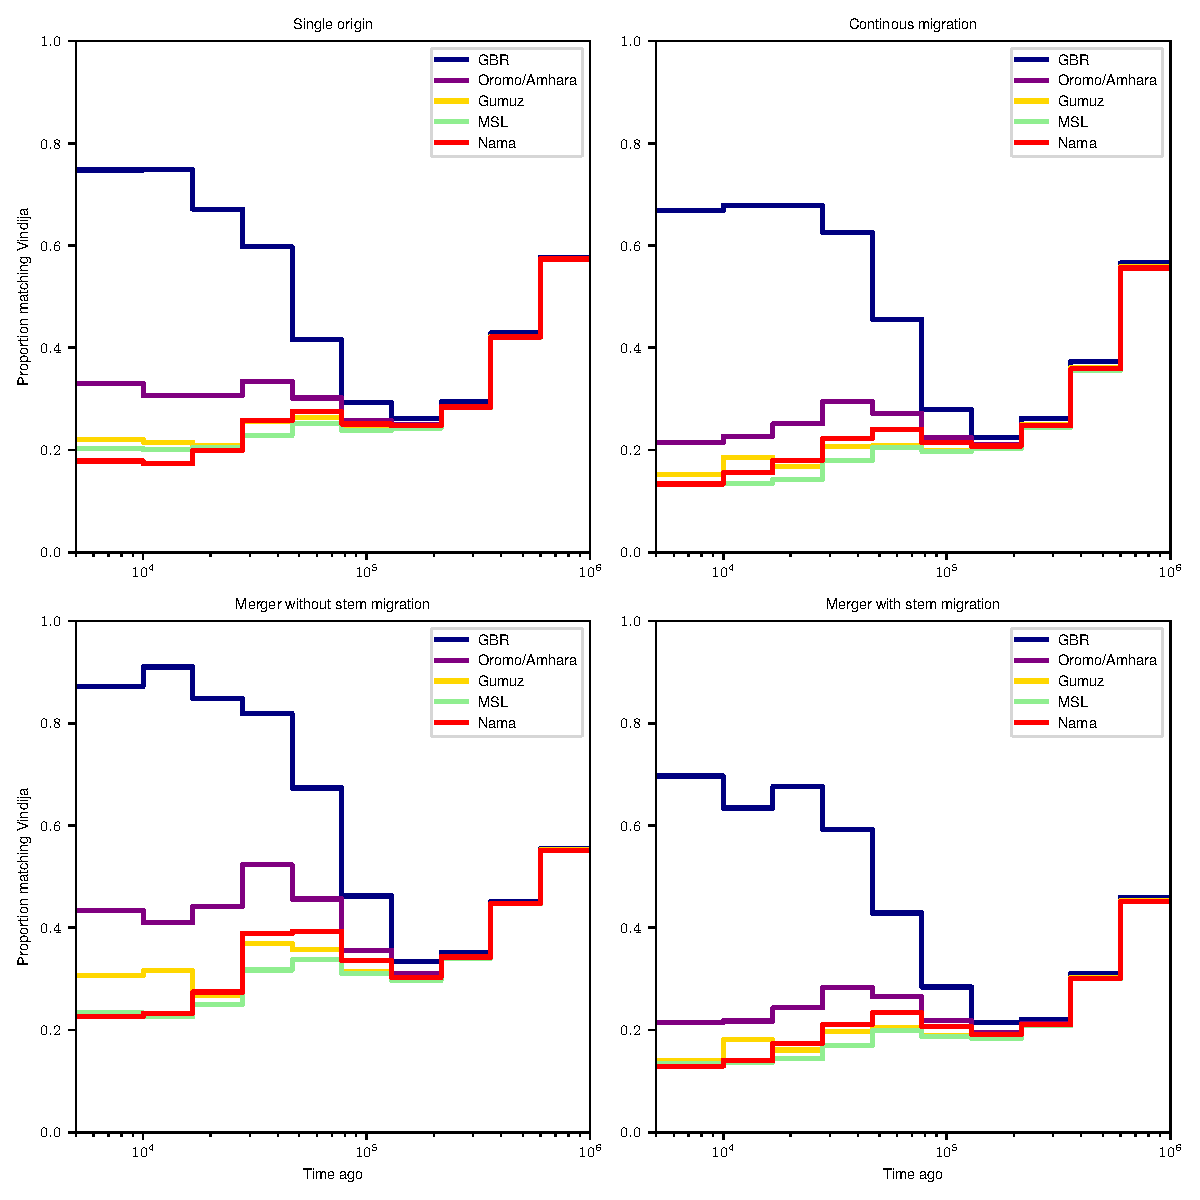
\includegraphics[width=\textwidth]{figures/supp-deep-branches-sim}
    \caption{
        \textbf{Deep branch distribution reinferred from simulated data.} We
        used Relate to reinfer gene genealogies from simulated data under the
        four highlighted models and categorized Neanderthal-matching deep
        branches in the simulated datasets. Each model provided a qualitative
        match to the data (highest proportion of Neanderthal-matching deep
        branches in the British, followed by Amhara/Oromo and Nama). Similar to
        reinferred IIRC and RCCR, no model provided a perfect match to the
        reconstructions using Relate with the data, but the similarities
        between reconstructed genealogies in the simulated data suggest such
        coalescence-rate based curves are underpowered to differentiate between
        plausible models of history.
    }
    \label{fig:supp-deep-branches-sim}
\end{figure}

\begin{figure}[ht]
    \centering
    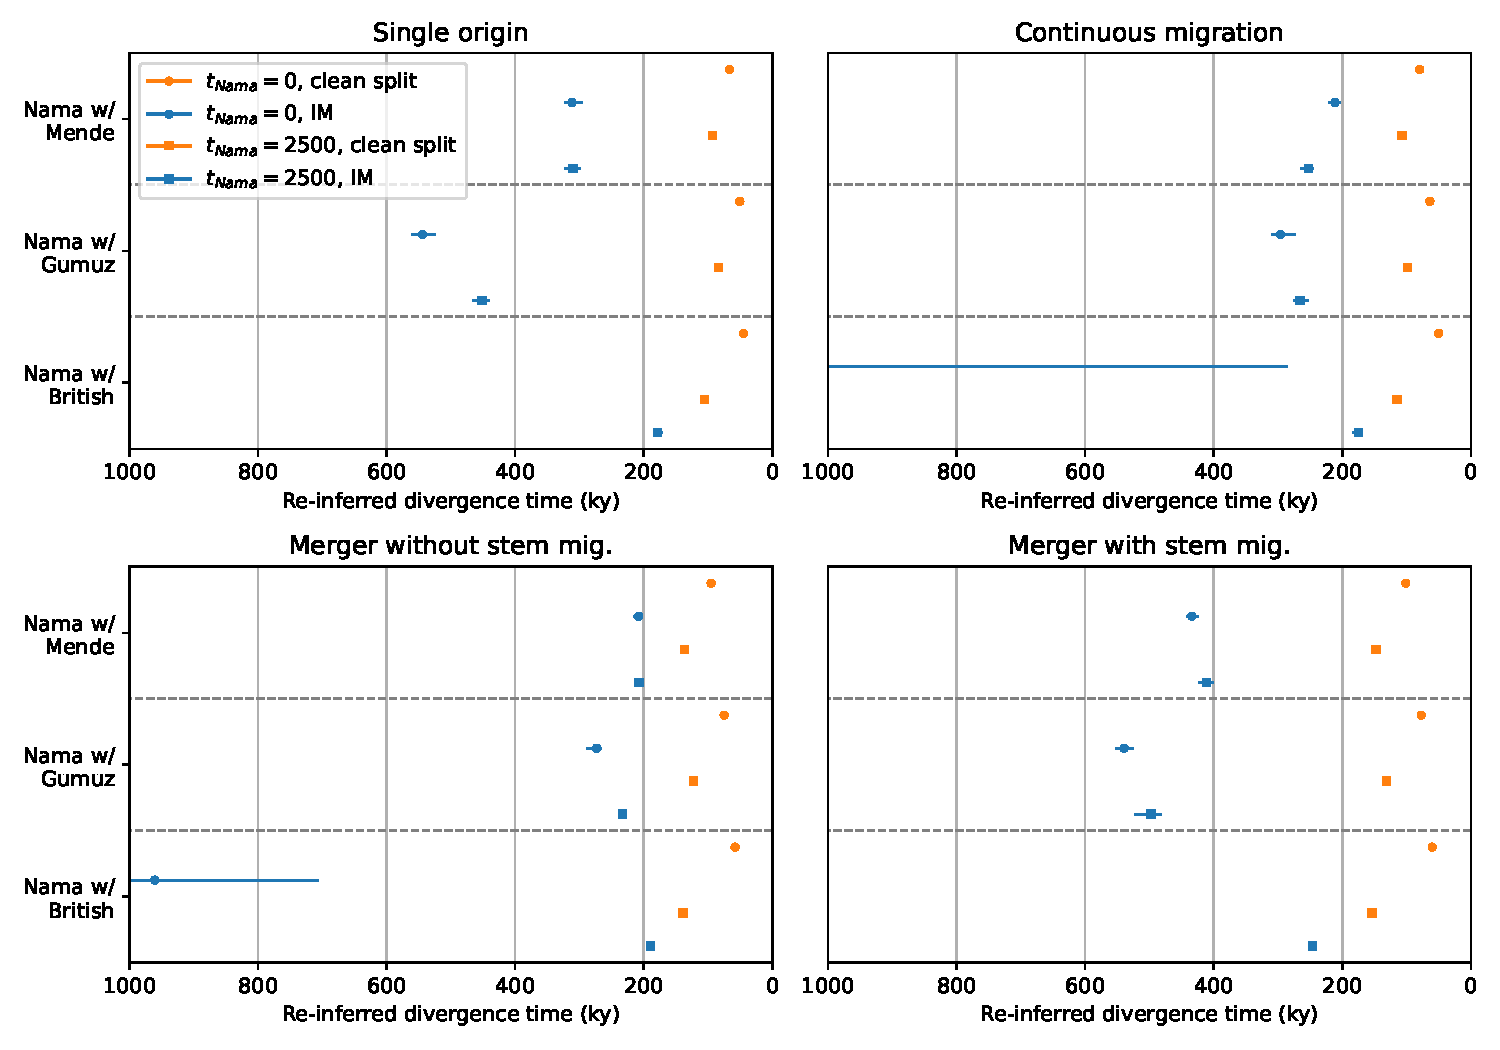
\includegraphics[width=\textwidth]{figures/supp-IM-misspecification}
    \caption{
        \textbf{IM model split times reinferred from simulated data of full
        model.} We simulated 10 diploid individuals under the four highlighted
        models (Sec.~\ref{sec:IM-reinfer}). Using the joint-SFS, we reinferred
        a simpler isolation-with-migration (IM) model for pairs of populations
        including the Nama to explore the effect of model mis-specification on
        the earliest inferred divergence times between Khoe-San and other
        populations. We simulated data with Nama individuals sampled at present
        ($t=0$) as well as Nama individuals sampled 2,500 years ago, prior to
        the recent gene flow from East Africans and Europeans. We fit two
        models for each model and population pair: one that allowed for
        migration between the populations (IM), and one that disallowed
        migration (clean split). Despite all original models having recent
        population divergences $\sim120$ka, the reinferred IM models all
        settled on divergence times greater than 200ka and sometimes much
        greater. If the true historical model includes reticulation or
        long-lasting structure, simpler IM models may be severely biased in
        favor of more ancient divergence times.
    }
    \label{fig:supp-IM-misspecification}
\end{figure}

\begin{figure}[ht]
    \centering
    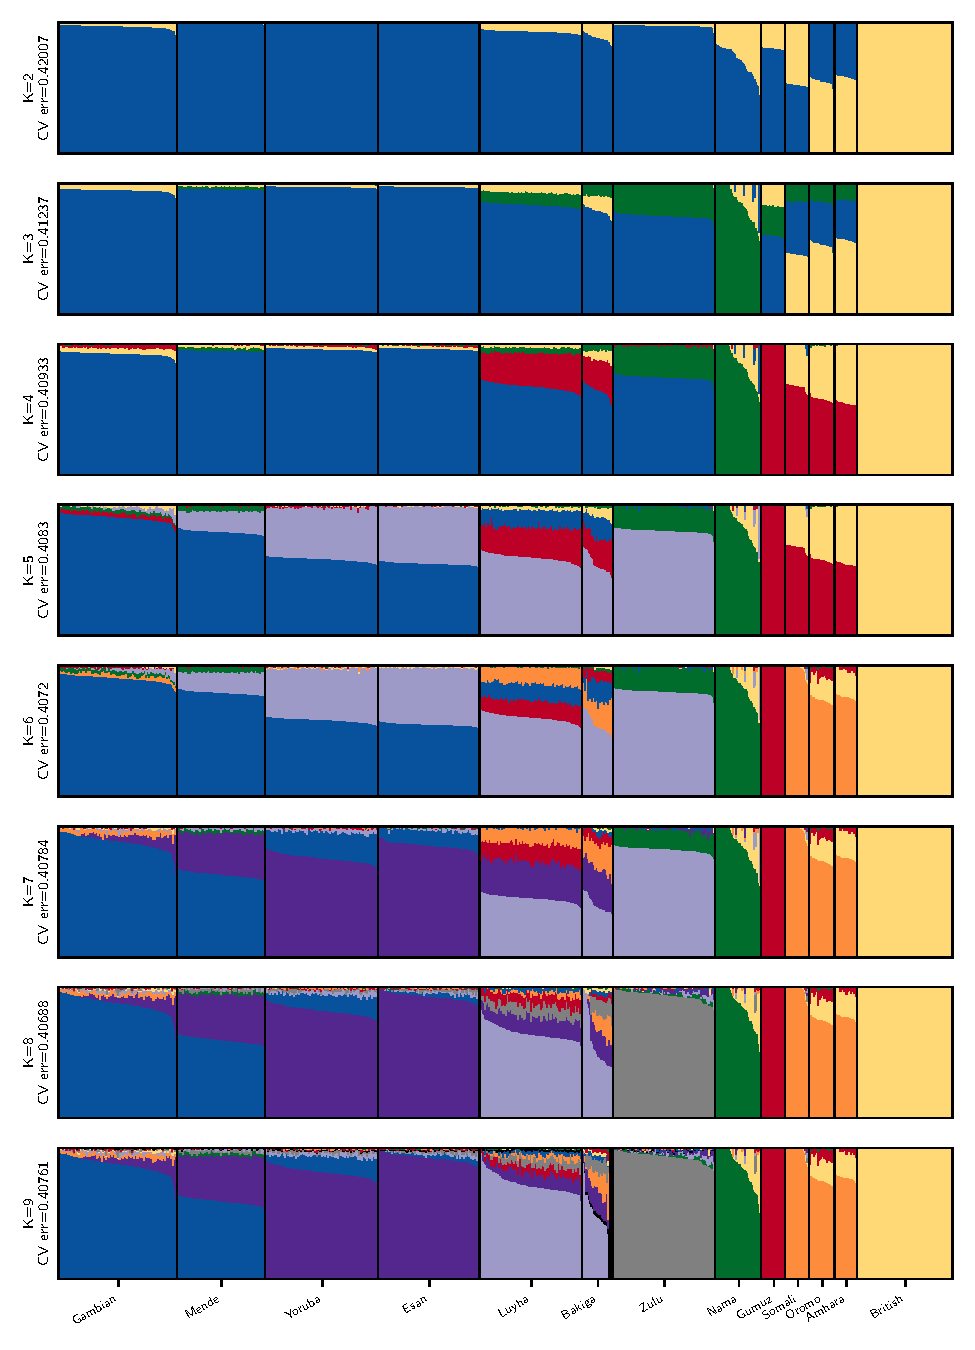
\includegraphics[width=5.75in]{figures/supp-admixture-panels}
    \caption{
        \textbf{\texttt{ADMIXTURE} clustering using $K=2$ to $9$ clusters.}
        \texttt{ADMIXTURE} \citep{Alexander2009-sw} was used to cluster all
        individuals in the subset of populations used in analyses in this
        paper. At $K=5$ clusters, West African populations begin to show
        variable separation in assigned clusters, likely due to
        isolation-by-distance demographic processes rather than recent
        admixture events. Figure~\ref{fig:diversity}D in the main text shows
        the \texttt{ADMIXTURE} results for $K=4$, which most clearly displays
        known admixture events in the histories of East and South African
        populations.
    }
    \label{fig:supp-admixture}
\end{figure}

\end{document}
